\documentclass[12pt]{article}

\usepackage[utf8]{inputenc}
%\usepackage[T1]{fontenc}

\usepackage{geometry}
\geometry{a4paper}
\usepackage{graphicx}
\usepackage{float}
\usepackage[italian]{babel}

%
%%%%%%%%%%%%%%%%%%%%%%%%%%%%%%%%%%%%%%%%%libreria per il disegno di curve 2D
\usepackage{tikz}
\usepackage{pgfplots}
\pgfplotsset{compat=newest}
\pgfplotsset{compat=1.11,
	/pgfplots/ybar legend/.style={
		/pgfplots/legend image code/.code={%
			\draw[##1,/tikz/.cd,yshift=-0.25em, xshift=0em]
			(0cm,0cm) rectangle (4pt,0.8em);},
	},
}

\usetikzlibrary{shapes,arrows,positioning,fit,patterns,fillbetween}

% Define bar chart colors
%
\definecolor{bblue1}{HTML}{ABBFD7}
\definecolor{bblue2}{HTML}{4F81BD}
\definecolor{ppurple1}{HTML}{BE94AC}
\definecolor{ppurple2}{HTML}{7D2A5A}

%
%%%%%%%%%%%%%%%%%%%%%%%%%%%%%%%%%%%%%%%%%libreria per l'uso del multiriga nelle tabelle
\usepackage{multirow}

%
%%%%%%%%%%%%%%%%%%%%%%%%%%%%%%%%%%%%%%%%%libreria per produrre pagine landscape in un documento principalmente portrait
\usepackage{pdflscape}

\usepackage{adjustbox}

\usepackage{subcaption}

%
%%%%%%%%%%%%%%%%%%%%%%%%%%%%%%%%%%%%%%%%%comando per la gestione semplificata di quotes
\newcommand{\quotes}[1]{``#1''}

%
%%%%%%%%%%%%%%%%%%%%%%%%%%%%%%%%%%%%%%%%%librerie per la visualizzazione del codice
\usepackage{listings}
\usepackage{xcolor}
\lstset{
	language=bash,
	basicstyle=\small\ttfamily\color{white},
	frame=tblr,
	backgroundcolor=\color{darkgray},
	xleftmargin=0.2em
}

\usepackage{pythonhighlight}

%
%%%%%%%%%%%%%%%%%%%%%%%%%%%%%%%%%%%%%%%%%libreria per l'inserimento di link nella
%   bibliografia
\PassOptionsToPackage{hyphens}{url}\usepackage[hidelinks]{hyperref}

\linespread{1.2}
\setlength{\parindent}{0pt}

\begin{document}

%----------------------------------------------------------------------------------------
%	TITOLO
%----------------------------------------------------------------------------------------

\begin{titlepage}

\newcommand{\HRule}{\rule{\linewidth}{0.5mm}}

\center

\textsc{\Large Relazione di progetto di \quotes{Smart City e Tecnologie Mobili}}\\[0.5cm]

\HRule \\[0.4cm]
{
	\huge \bfseries
	Rilevatore di sonnolenza\\
	all'interno di un autoveicolo con\\
	Raspberry Pi\\[0.4cm]
}
\HRule \\[1.5cm]

\vfill

\begin{flushleft}
\emph{Numero del gruppo:}\\
62\\[1cm]
\emph{Componenti del gruppo:}\\
Giacomo Frisoni\\
Marcin Pabich\\[3cm]
\end{flushleft}

\end{titlepage}

%----------------------------------------------------------------------------------------
%	INDICE
%----------------------------------------------------------------------------------------

\tableofcontents

\newpage

%----------------------------------------------------------------------------------------
%	INTRODUZIONE
%----------------------------------------------------------------------------------------

\section{Introduzione}

Il deterioramento delle capacità alla guida causato da sonnolenza è noto per essere uno dei fattori che contribuiscono maggiormente alla formazione di incidenti automobilistici. Secondo un sondaggio del 2011 realizzato dalla National Sleep Foundation sulla popolazione americana, circa il 30\% degli incidenti su strada è dovuto all'affaticamento del conducente e tale dato tende a crescere di anno in anno\cite{SleepInAmerica}. Una recente indagine svolta dalla NHTSA\footnote{NHTSA. National Highway Traffic Safety Administration.} ha inoltre stimato un numero complessivo di 90.000 incidenti in America segnalati dalla polizia nel 2015 (con 41.000 feriti e più di 800 morti), aventi come causa l'insorgere di uno stato di sonnolenza\cite{NHTSA}.\\
La sonnolenza costituisce nello specifico una fase di transizione nel ciclo sonno-veglia, determinante uno stato di torpore e una riduzione del livello di coscienza della persona. Nell'ambito in esame, la sonnolenza deteriora le prestazioni del guidatore e può infine portare all'incapacità di resistere al sonno al volante. Essa può essere dovuta a diversi fattori: condizioni di guida avverse, traffico intenso, alti carichi di lavoro, scarso riposo, orari notturni, disturbi del sonno, abuso di alcol e assunzione di medicinali sono solo alcuni esempi. Tutti questi fattori hanno effetti cumulativi e una loro combinazione può aumentare in modo sostanziale il rischio di incidenti stradali. Gli aspetti critici su cui impatta la sonnolenza alla guida, invece, sono i tempi di reazione, la vigilanza, il livello di attenzione e la velocità nell'elaborare le informazioni.\\
A partire dal 1995 i ricercatori hanno iniziato a concentrare i propri sforzi sulla costruzione di dispositivi di allarme, come una tra le principali tecniche di contromisura. L'obiettivo di questi sistemi è quello di allarmare o risvegliare i conducenti che sono assonnatti o addormentati, riducendo conseguentemente la percentuale di scontri e avvenimenti inattesi sul suolo stradale. Una carenza intrinseca in tutti i tipi di dispositivi di allarme, tuttavia, è da ricercarsi nel fatto che molte persone continuano a guidare anche quando sanno di essere sonnolenti, lottando per rimanere svegli. Sebbene un dispositivo di allarme efficace possa prevenire un incidente, un autista che si addormenta una volta rischia di addormentarsi nuovamente a meno che non smetta di guidare. Da diversi anni gli esperti di sicurezza hanno espresso preoccupazione sul fatto che i dispositivi di allarme possano fornire ai conducenti un falso senso di sicurezza, incoraggiandoli a guidare per lungo tempo\cite{DrowsyDrivingReport}.\\
Il progetto descritto in questo documento si pone l'obiettivo di realizzare un sistema a basso costo, affidabile e non intrusivo per il riconoscimento della stanchezza del conducente in tempo reale, svolgendo un monitoraggio video sul suo volto e applicando tecniche di Computer Vision sui frame catturati. L'implementazione della soluzione si basa sull'uso di un \textit{Raspberry Pi 3 B}, un single-board computer noto per le sue caratteristiche prestazionali rapportate al prezzo e alle dimensioni che lo contraddistinguono.\\
Il sistema acquisisce le immagini dell'utente per mezzo di una camera installata nell'automobile e posizionata frontalmente a esso. La sonnolenza del guidatore è successivamente calcolata in riferimento a una misura comportamentale incentrata sulla chiusura degli occhi (stimata quantitativamente con metodologia \textit{EAR}\footnote{EAR. Eye Aspect Ratio.}\cite{EAR}). A fronte di una chiusura degli occhi protrattasi oltre un tempo definito, il sistema riproduce un allarme per mezzo di un buzzer acustico al fine di reclamare l'attenzione dell'utente ed evidenziare il potenziale pericolo che sta incorrendo.\\
Le principali tecnologie adottate sono \textit{Python} a livello di linguaggio di programmazione, \textit{OpenCV}\cite{OpenCV} come libreria per la manipolazione di foto e video, \textit{dlib}\cite{Dlib} per quanto concerne gli algoritmi di machine learning per l'individuazione e la localizzazione di facial landmark.\\
Il contributo tecnologico/scientifico apportato dal gruppo con l'elaborato in esame si riferisce allo studio e al confronto prestazionale delle varie soluzioni che possono essere implementate, specie in relazione ai limiti dell'hardware adottato. Una particolare attenzione è riposta nelle tecniche di riconoscimento facciale: esse rappresentano la base dell'intero processo e sono note per essere l'elemento centrale sia per la determinazione dell'efficacia del sistema nei vari scenari d'uso che per la sua reale efficienza.

\iffalse
Esporre l’obiettivo del progetto dandone una visione complessiva.\\
Devono essere illustrate le caratteristiche salienti del progetto; deve essere chiara la distinzione tra le tecnologie usate/assemblate durante lo svolgimento dell’elaborato e il contributo tecnologico/scientifico effettivamente apportato dal gruppo.\\

Vincoli circa la lunghezza della sezione (escluse didascalie, tabelle, testo nelle immagini, schemi):

\vspace{1cm}
\begin{tabular}{l|rr}
	& Numero minimo di battute & Numero massimo di battute \\
	\hline
	1 componente & 2000 & 3000 \\
	2 componenti & 2500 & 4500 \\
	3 componenti & 3000 & 6000 \\
	\hline
\end{tabular}
\fi

\newpage


%----------------------------------------------------------------------------------------
%	STATO DELL'ARTE
%----------------------------------------------------------------------------------------

\section{Stato dell'arte}

Misurare direttamente il livello di sonnolenza è complesso. Esistono tuttavia numerosi metodi indiretti capaci di rilevare aspetti correlati e che oggi costituiscono la base per i vari sistemi disponibili sul mercato.
In questa sezione si riportano le soluzioni presenti in letteratura per quanto concerne il problema in esame, distinguendole sulla base del tipo di misura su cui si basano (riassunte in Figura \ref{fig:StateOfTheArt}). Inoltre si citano quelle già operative sul mercato: lo sviluppo di tecnologie per il rilevamento di sonnolenza, infatti, costituisce una sfida sia accademica che industriale.

\subsection{Misure fisiologiche}

Le misure di segnali fisiologici comprendono tecniche quali ECG (elettrocardiogramma), EOG (elettrooculogramma), EEG (elettroencefalogramma) e HRV\footnote{HRV. Heart Rate Variability.}.
Il segnale EEG, in particolare, è il più utilizzato nella classe fisiologica per la misurazione della stanchezza. Esso fornisce informazioni sull'attività del cervello e consente pertanto di individuare la perdita di concentrazione e il rallentamento dei tempi di risposta tipici di chi è affetto da affaticamento e sonnolenza. Il segnale EEG ha varie bande di frequenza: \textit{delta} (0,5-4 Hz) - corrispondente al sonno, \textit{theta} (4-8 Hz) - legata alla stanchezza, \textit{alpha} (8-13 Hz) - rappresentante uno stato di rilassamento e creatività, \textit{beta} (13-25 Hz) - corrispondente a uno stato di vigilanza. Una diminuzione della variazione di potenza nella banda di frequenza \textit{alpha} e un relativo aumento in \textit{theta} è pertanto indice di sonnolenza. Secondo uno studio condotto nel 2011\cite{EEG}, le tecniche EEG sono le più accurate, con un tasso di precisione superiore al 90\%. Tuttavia, le misure fisiologiche faticano a essere adottate nella realtà a causa dei loro costi, della connessione fisica che richiedono con l'autista e dello stress indotto tipicamente nell'utente che indossa le apparecchiature di monitoraggio necessarie. Una soluzione più pratica è stata studiata per Jaguar Land Rover\cite{Jaguar}.

\subsection{Misure basate sul veicolo}

La maggior parte delle soluzioni attualmente disponibili e impiegate dalle case automobilistiche riguardano misure basate sul veicolo e comprendono pertanto l'individuazione di scostamenti rispetto alla propria corsia, la pressione esercitata sui pedali e il movimento delle ruote sterzanti. Si tratta dunque di approcci basati su modelli di guida che hanno lo svantaggio di dipendere fortemente dalle caratteristiche del veicolo, dalle condizioni della strada e dalle capacità del conducente.\\
In un paper del 2009\cite{SWM} un gruppo di ricercatori ha rilevato il livello di sonnolenza con un'accuratezza dell'86\%, considerando le correlazioni tra le micro-regolazioni esercitate sul volante per il mantenimento dell'automobile (individuate grazie a sensori per la misurazione dell'angolo di sterzata) in corsia e l'affaticamento del guidatore stesso. Tale tecnica di rilevamento è denominata SWM\footnote{SWM. Steering Wheel Movement.}.\\
Un'altra misura basata sul veicolo spesso utilizzata per misurare la sonnolenza del conducente è SDLP\footnote{SLDP. Standard Deviation of Lane Position.}, dove la posizione della corsia viene tracciata per mezzo di una telecamera esterna. Il principale limite di questa tecnica risiede nella dipendenza da fattori quali la segnaletica orizzontale, l'illuminazione e le condizioni climatiche.\\
I sistemi implementati oggi all'interno delle automobili di fascia alta tengono in genere conto di un insieme di parametri. Il Driver Alert di Ford\cite{Ford}, il Safety-IBuzz Fatigue Alert di Skoda\cite{Skoda} e il Bosch Driver Drowsiness Detection System\cite{Bosch} adottato da Volkswagen sono i più conosciuti esempi industriali.

\subsection{Misure comportamentali}

Le soluzioni basate su misure di tipo comportamentale sono le più diffuse negli ultimi anni. Esse si basano sulle caratteristiche tipiche del movimento facciale nelle persone assonnate: rapidi e costanti battiti di ciglia, chiusura degli occhi, annuenza o oscillazione della testa e frequenti sbadigli. La maggior parte degli studi pubblicati sugli approcci comportamentali per la determinazione della sonnolenza si focalizza sul battito di ciglia. Sotto questo punto di vista, la misura del PERCLOS\footnote{PERCLOS. Percentuale di chiusura della palpebra sopra la pupilla nel tempo. Riflette la tipica chiusura rallentata degli occhi nei soggetti affetti da sonnolenza.} costituisce la tecnica più diffusa e impiegata anche nell'ambito dei prodotti commerciali.\\
Il principale limite legato all'uso di tecniche di Computer Vision per l'estrazione di feature facciali è l'illuminazione. Le camere normali non consentono di ottenere risultati soddisfacenti in scenari notturni. Per ovviare il problema, alcuni ricercatori hanno fatto uso di una illuminazione infrarossi tramite LED\footnote{LED. Light Emitting Node.}\cite{IEEE} (che consente buone prestazioni di notte ma è meno robusta durante il giorno). Le immagini vengono acquisite dalla camera a un certo frame rate, elaborate per garantire prima l'estrazione del volto e poi per localizzare la specifica regione d'interesse (ad esempio tramite Haar Cascade Classifier o HOG) su cui realizzare il calcolo della misura scelta. Approcci più recenti, infine, si basano su Deep Learning.

\begin{figure}
	\begin{subfigure}{.4\textwidth}
		\centering
		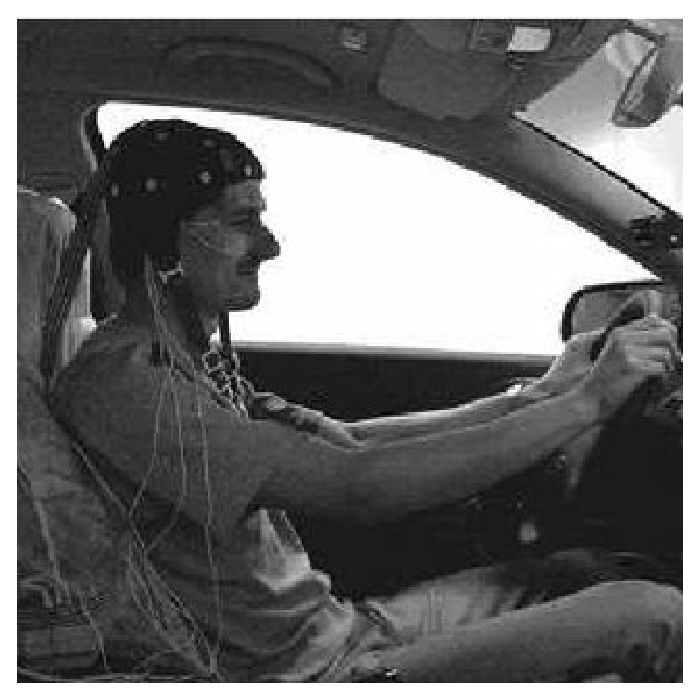
\includegraphics[width=.8\linewidth]{eps/eeg.eps}
		\caption{Esempio pratico di misura fisiologica con casco EEG.}
	\end{subfigure}
	\hspace{5mm}
	\begin{subfigure}{.55\textwidth}
		\centering
		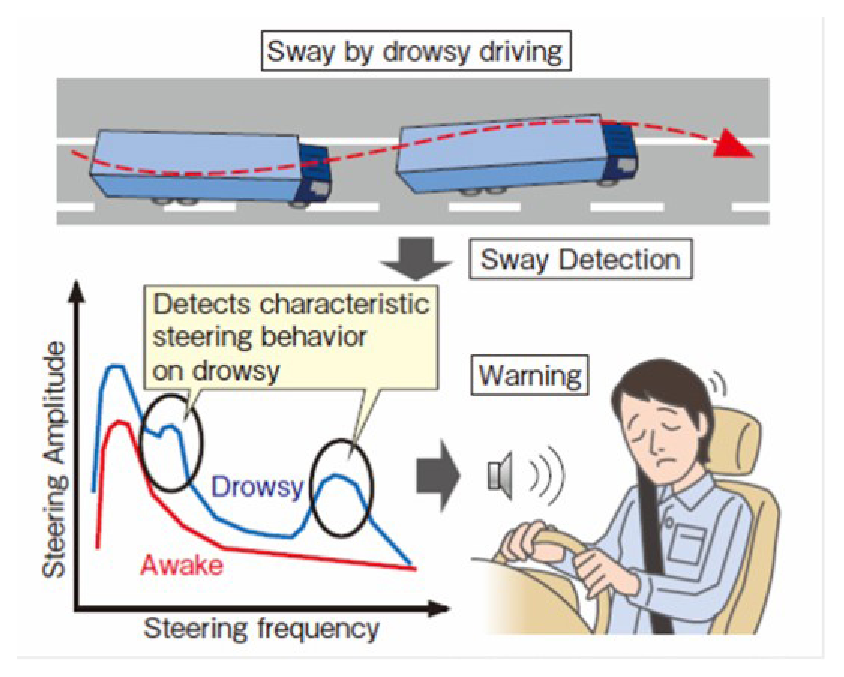
\includegraphics[width=.8\linewidth]{eps/swm.eps}
		\caption{Funzionamento della misura SWM\\basata sul veicolo.}
	\end{subfigure}
	\par\bigskip % force a bit of vertical whitespace
	\begin{subfigure}{.55\textwidth}
		\centering
		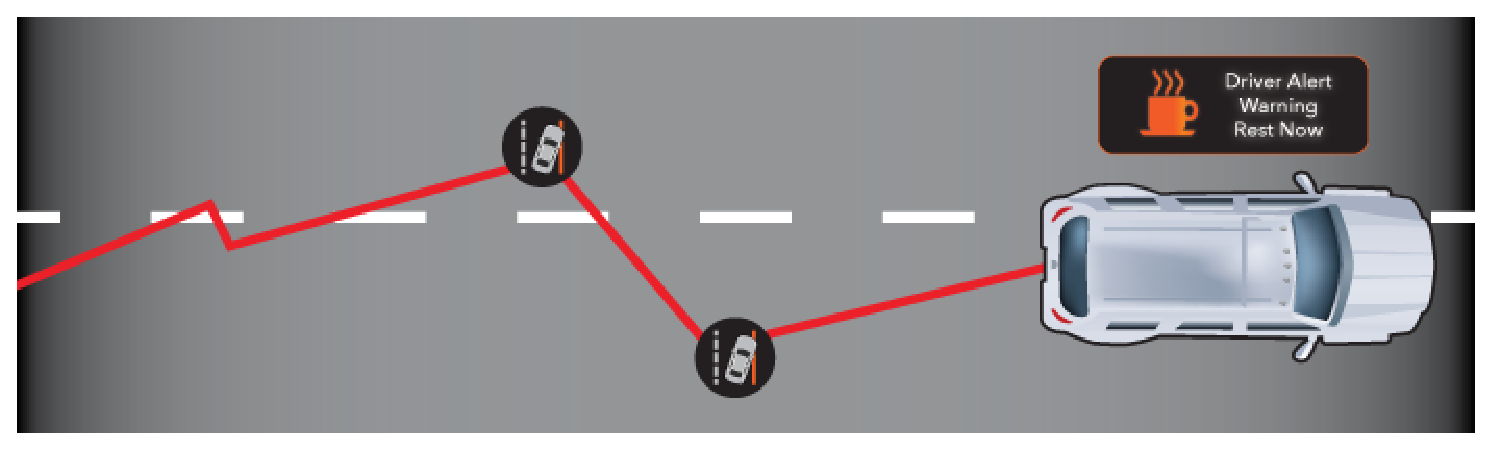
\includegraphics[width=.8\linewidth]{eps/sdlp.eps}
		\caption{Funzionamento della misura SLDP basata\\sul veicolo.}
	\end{subfigure}
	\begin{subfigure}{.4\textwidth}
		\centering
		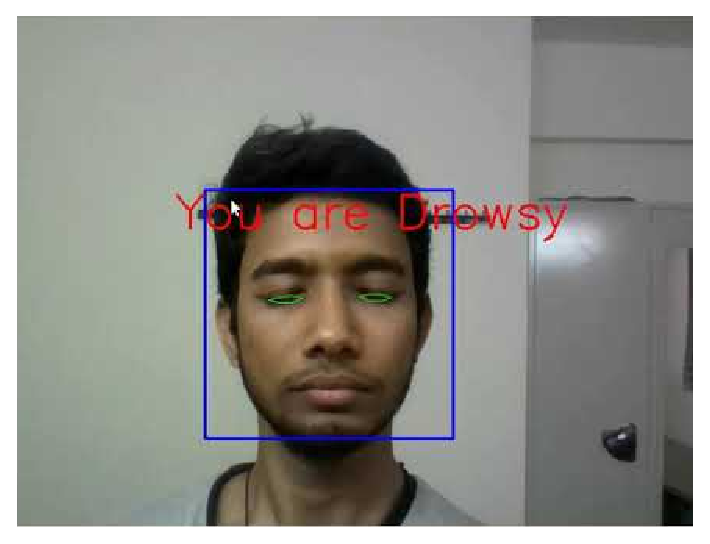
\includegraphics[width=.8\linewidth]{eps/ear.eps}
		\caption{Misure comportamentale incentrate sulla chiusura degli occhi calcolata con tecniche di Computer Vision.}
	\end{subfigure}
	\par\bigskip % force a bit of vertical whitespace
	\begin{subfigure}{\textwidth}
		\centering
		\includegraphics[width=.5\linewidth]{eps/volkswagen_alert.eps}
		\caption{Avviso di sonnolenza all'interno dei veicoli Volkswagen\cite{Volkswagen}.}
	\end{subfigure}
	\caption{Esempi di soluzioni per il rilevamento della sonnolenza alla guida, con distinzione nella misura adottata.}
	\label{fig:StateOfTheArt}
\end{figure}

\subsection{Confronto col progetto presentato}
Il progetto analizzato in questa relazione realizza il rilevamento della sonnolenza attraverso una misura comportamentale incentrata sulla chiusura degli occhi del conducente. Si basa pertanto su tecniche di Computer Vision sia per la \textit{face detection} che per l'estrazione dei \textit{facial landmark}. L'apertura degli occhi è calcolata mediante l'EAR, una soluzione diffusa in letteratura (come alternativa al PERCLOS) e nota per i suoi vantaggi: stima incentrata su una sola grandezza scalare, superamento dei risultati allo stato dell'arte su due dataset standard, e ricavabile attraverso una semplice formula da una sola immagine. L'adozione del Raspberry Pi 3 B come piattaforma hardware di riferimento vincola in misura maggiore rispetto alle soluzioni presentate l'applicabilità di algoritmi di visione, costringendo a considerare con massimo riguardo il trade-off tra accuratezza e velocità d'elaborazione (real-time per requisito).

\iffalse
Riassumere le soluzioni presenti in letteratura inerenti al problema in esame. Per ciascuna, discutere le principali diversità o affinità rispetto al progetto presentato. Nel caso non siano presenti soluzioni direttamente comparabili a quella presentata descrivere comunque le principali tecniche note per affrontare la tematica trattata.\\

Le soluzioni esposte devono essere corredate degli opportuni riferimenti bibliografici. Nel caso si tratti di soluzioni già operative sul mercato, devono essere indicate le fonti (online) dove poter accedere al servizio o approfondirne i contenuti.\\

Vincoli circa la lunghezza della sezione (escluse didascalie, tabelle, testo nelle immagini, schemi):

\vspace{1cm}
\begin{tabular}{l|rr}
 & Numero minimo di battute & Numero massimo di battute \\
 \hline
 1 componente & 2000 & 3000 \\
 2 componenti & 2500 & 4500 \\
 3 componenti & 3000 & 6000 \\
 \hline
\end{tabular}
\fi

\newpage


%----------------------------------------------------------------------------------------
%	ANALISI DEI REQUISITI
%----------------------------------------------------------------------------------------

\section{Analisi dei requisiti}
\label{sec:requisiti}

In questa sezione sono trattati in modo dettagliato tutti i requisiti del progetto, emersi durante la fase di analisi.

\subsection{Business Requirements}
\begin{enumerate}
	\item Realizzare un progetto di qualità sia nella sua parte software che hardware, valutandone accuratamente le prestazioni.
	\item Organizzare il lavoro in team, definendo un apposito piano e sperimentando la suddivisione di task mediante diagramma di Gantt.
	\item Mettere alla prova le conoscenze acquisite durante il corso relative ai sistemi embedded, al Raspberry Pi, alla videosorveglianza e alle tecnologie di sensing.
\end{enumerate}

\subsection{User Requirements}
\begin{enumerate}
	\item Possibilità di posizionare il dispositivo all'interno del veicolo, frontalmente al conducente.
	\item Capacità del sistema di riconoscere il livello di sonnolenza del guidatore, considerando una misura comportamentale basata sulla chiusura degli occhi.
	\begin{enumerate}
		\item Il sistema deve considerare il guidatore in uno stato di sonnolenza e pertanto in una situazione di pericolo se la chiusura dei suoi occhi si protrae per un tempo eccessivo.
		\item Nella misurazione della sonnolenza, il sistema deve tener conto della reale apertura di ambo gli occhi.
	\end{enumerate}
	\item Avvio automatico del sistema all'atto dell'alimentazione.
	\item Attivazione o disattivazione del rilevamento su richiesta del conducente.
	\begin{enumerate}
		\item Il sistema deve procedere al monitoraggio del volto del conducente, al rilevamento del suo grado di sonnolenza e alla segnalazione di scenari di pericolo solo se attivo.
	\end{enumerate}
	\item Gestione degli scenari d'uso legati al riconoscimento del volto.
	\begin{enumerate}
		\item Volto rilevato. Il sistema deve procedere con la misura dell'indice di sonnolenza.
		\item Volto non rilevato. Il sistema non deve produrre allarmi, evitando segnalazioni potenzialmente non connesse a situazioni di reale pericolosità.
		\item Volto non rilevato, sonnolenza precedentemente rilevata. Il sistema continua a produrre allarmi nel caso in cui ha rilevato la sonnolenza nel soggetto prima di perdere traccia del suo volto.
	\end{enumerate}
	\item Segnalazione acustica e visiva degli scenari di pericolo rilevati.
\end{enumerate}

\subsection{Functional Requirements}
\begin{enumerate}
	\item Il sistema deve monitorare il viso dell'utente attraverso una camera.
	\item La misurazione della sonnolenza del conducente deve avvenire grazie a tecniche di Computer Vision.
	\begin{enumerate}
		\item Il sistema deve applicare tecniche di face recognition per l'individuazione del volto.
		\item Il sistema deve applicare tecniche di facial landmarking per l'individuazione delle sole coordinate di interesse per quanto concerne gli occhi.
		\item Il sistema deve rilevare la chiusura degli occhi nei vari frame grazie al calcolo dell'EAR per ognuno di essi.
		\item Si considera la presenza di uno scenario di pericolo nel momento in cui la misura dell'EAR indica la chiusura degli occhi per un definito numero di frame consecutivi, ritenuto di adatta sensibilità per gli obiettivi del sistema.
	\end{enumerate}
	\item Il sistema deve avviare il software di rilevamento nella fase di reboot, indicando opportunamente, tramite segnali luminosi, lo stato in cui si trova:
	\begin{enumerate}		
		\item Loading (LED giallo acceso). Il sistema è in fase di caricamento, non è possibile interagire con esso.
		\item Ready (LED verde acceso). Il sistema è pronto a ricevere l'input dal conducente.
		\item Working (LED videocamera acceso). Il sistema sta acquisendo ed analizzando le immagini per la rilevazione dei colpi di sonno.
		\item Alert (LED rosso acceso). Il sistema ha rilevato una potenziale situazione di pericolo.
	\end{enumerate}
	\item Il sistema deve consentire l'avvio o l'arresto della rilevazione mediante la pressione di un pulsante.
	\begin{enumerate}
		\item L'acquisizione dei frame dalla camera e la loro successiva elaborazione devono avvenire solo se il sistema è attivo.
	\end{enumerate}
	\item Il sistema deve adottare un comportamento idoneo sia a fronte del riconoscimento del volto che del fallimento di tale fase.
	\begin{enumerate}
		\item Volto rilevato. Il sistema deve procedere con l'estrazione dei facial landmark e il calcolo dell'EAR per entrambi gli occhi.
		\item Volto non rilevato. Il sistema deve procedere con l'analisi dei successivi frame, senza segnalare situazioni di pericolo.
		\item Volto non rilevato, sonnolenza precedentemente rilevata. Il sistema deve procedere a segnalare la situazione di pericolo rilevata prima di perdere traccia del volto.
	\end{enumerate}
	\item Il sistema deve segnalare al conducente la presenza di uno scenario di pericolo causato dal rilevamento di sonnolenza, adottando due tipologie distinte di avvertimento.
	\begin{enumerate}
		\item Avvertimento acustico, per mezzo di un buzzer sonoro.
		\item Avvertimento visivo, per mezzo di un LED.
	\end{enumerate}
\end{enumerate}

\subsection{Non-functional Requirements}
\begin{enumerate}
	\item \textbf{Dimensioni.} Il sistema deve avere dimensioni conformi per una sua installazione a bordo di un autoveicolo, in modo da non ostacolare in alcun modo la guida. L'intera soluzione deve pertanto essere facile da trasportare e poco ingombrante.
	\item \textbf{Real-time.} Il sistema deve essere in grado di elaborare i frame catturati e di fornire segnalazioni di pericolo in tempo reale, specie in considerazione della velocità con cui il veicolo potrebbe essere in movimento. Ciò ha impatto sia sulla scelta dell'hardware - che deve risultare di sufficiente capacità computazionale - sia sulla progettazione del software - che non deve rivelarsi eccessivamente complesso nel rispetto delle limitate risorse che si hanno a disposizione sulla piattaforma scelta.
	\item \textbf{Affidabilità.} Il rilevamento della sonnolenza del conducente deve avvenire nel modo più accurato possibile, riducendo al minimo il numero di falsi positivi e consentendo solo ridotti margini di errore. Il sistema deve essere robusto a eventuali variazioni dell'ambiente, della luminosità e dell'orientamento del volto. Ove possibile, inoltre, l'oggettistica, gli indumenti indossati e la colorazione della pelle del guidatore non devono compromettere il funzionamento del sistema stesso.
\end{enumerate}

\subsection{Implementation Requirements}
\begin{enumerate}
	\item \textbf{Raspberry Pi 3 B.} La componente hardware del sistema deve essere basata su Raspberry Pi 3 B, un single-board computer economico, di ridotte dimensioni e di buone capacità computazionali. La ragione alla base di tale scelta è da ricercarsi nella volontà di approfondire le conoscenze apprese durante il corso di Smart City e Tecnologie Mobili, acquisendo anche esperienza nello sviluppo di progetti basati su questo tipo di piattaforma. Inoltre la scelta legata all'impiego di tale dispositivo è stata operata in funzione delle disponibilità in termini di risorse del laboratorio universitario.
	\item \textbf{RaspiCam v 1.3.} La cattura dei video raffiguranti l'utente alla guida deve essere realizzata mediante la versione 1.3 di RaspiCam (modulo di camera ufficiale per Raspberry Pi). La scelta legata all'uso di tale hardware, analogamente al caso di Raspberry Pi 3 B, è stata realizzata a fronte della visione del materiale disponibile per gli studenti del corso.
	\item \textbf{Budget.} La realizzazione del sistema deve avvenire a basso costo da un punto di vista economico in tutte le sue componenti, nell'ottica anche di un ipotetico deployment su larga scala.
	\item \textbf{Tempi di sviluppo.} Il completamento del progetto deve avvenire considerando un monte ore di lavoro complessivo pari a 100 per ogni studente.
\end{enumerate}

\iffalse
In questa sezione esporre brevemente i requisiti a cui il sistema proposto deve rispondere, concentrando l'attenzione sugli aspetti più rilevanti e facendo eventualmente uso di opportuni diagrammi di alto livello.\\

Vincoli circa la lunghezza della sezione (escluse didascalie, tabelle, testo nelle immagini, schemi):

\vspace{1cm}
\begin{tabular}{l|rr}
 & Numero minimo di battute & Numero massimo di battute \\
 \hline
 1 componente & 4000 & 6000 \\
 2 componenti & 6000 & 8000 \\
 3 componenti & 8000 & 10000 \\
 \hline
\end{tabular}
\fi


\newpage


%----------------------------------------------------------------------------------------
%	PROGETTAZIONE
%----------------------------------------------------------------------------------------

\section{Progettazione}
\label{sec:progettazione}

In questa sezione sono esposte le scelte progettuali operate nelle varie fasi di sviluppo dell'elaborato.

\subsection{Metodologia}

La metodologia alla base del progetto si compone di tre parti fondamentali: (1) rilevamento del volto (\textit{face detection}), (2) rilevamento dei punti di riferimento facciali (\textit{facial landmark detection}) e (3) rilevamento della sonnolenza. Ciascuno di questi problemi può essere affrontato con diversi approcci risolutori noti in letteratura. Dal momento che ogni tecnica possiede sia aspetti positivi che negativi, la scelta di quale adottare per il problema di riferimento deve essere frutto di un'attenta analisi in funzione dei requisiti che si devono soddisfare (già evidenziati nella sezione \ref{sec:requisiti}). La valutazione e lo studio delle soluzioni che possono essere intraprese nelle fasi metodologiche costituiscono pertanto due elementi chiave per una valida progettazione. Esse assumono inoltre un ruolo preponderante nella determinazione del successo o del fallimento degli obiettivi stabiliti dall'elaborato stesso. Nei successivi paragrafi si discutono in maggior dettaglio le problematiche emerse sul piano progettuale e si giustificano le scelte intraprese.

\subsubsection{Rilevamento del volto}
\label{subsubsec:face_detection}

Rilevare la presenza del volto del conducente e localizzarne la posizione all'interno di un'immagine rappresenta un'operazione centrale in tutti i progetti di \textit{drowsiness detection} basati su misure comportamentali e, quindi, algoritmi principalmente connessi alla Computer Vision. I localizzatori allo stato dell'arte più utilizzati in letteratura e considerati d'interesse ai fini del progetto sono di seguito riportati, classificandoli nelle due principali famiglie con cui possono essere distinti.
\begin{itemize}
	\item \textbf{Tecniche feature-based}. Usano esplicitamente la conoscenza dell'aspetto del volto, caratterizzato da un insieme di feature di basso livello: proprietà dei pixel, informazioni sulla geometria del volto e modelli standard definiti manualmente o descritti da funzioni (\textit{template matching}).
	\item \textbf{Tecniche image-based}. Affrontano il problema della localizzazione del volto come un generico problema di pattern recognition dove l'obiettivo è imparare a riconoscere l'immagine di un viso sulla base di alcuni esempi di training.
	\begin{itemize}
		\item \textbf{Haar Cascade Classifier.}\\
		È una tecnica di Machine Learning proposta da Paul Viola e Michael Jones nel 2001\cite{Haar}, introdotta per la localizzazione di oggetti e applicata poi con successo all'individuazione di volti. Il localizzatore di Viola e Jones, nello specifico, è uno dei più robusti ed efficienti allo stato dell'arte. La procedura d'individuazione del volto, infatti, consente un funzionamento real-time. Tuttavia l'addestramento è molto lento (può richiedere giorni) e necessita di numerose istanze sia di esempi positivi che negativi.
		Internamente utilizza un classificatore in grado di associare un pattern in input a una delle due classi volto e non volto. Ciò è possibile poichè le immagini contenenti volti hanno proprietà comuni, mentre quelle che non li rappresentano sono estremamente irregolari.
		\begin{itemize}
			\item \textbf{Haar-like feature.}\\
			La localizzazione dei volti avviene analizzando sottofinestre consecutive (sovrapposte e di dimensione variabile) dell'immagine in input, estraendo le feature presenti nella finestra e classificando la finestra stessa come volto o non volto. Le feature Haar-like sono caratterizzate dall'applicazione di regioni rettangolari di colorazione bianca e nera unite tra loro, come mostrato in Figura \ref{fig:haar_features}. Ogni feature è posizionata in una sottoregione di una sottofinestra dell'immagine e il suo valore è calcolato come somma pesata di due componenti: la somma dei pixel nella regione nera e la somma di quelli interni alla ragione bianca. I segni dei due pesi sono opposti e i loro valori assoluti sono inversamente proporzionali alle aree delle rispettive regioni, in modo da effettuare un calcolo normalizzato. Le feature Haar-like, inoltre, sono applicate modificandone la dimensione, la forma e la posizione nella sottofinestra. Il motivo legato al loro uso è da ricercarsi nella loro efficacia ai fini della localizzazione del volto e nell'efficienza con cui possono essere calcolate mediante l'impiego dell'immagine integrale. Nonostante la rapidità con cui è possibile individuarle, occorre osservare come a ogni sottofinestra possano nella pratica corrispondere diverse miliaia di feature associate.
			\item \textbf{Immagine integrale.}\\
			Le semplici feature rettangolari di un'immagine sono calcolate utilizzando una rappresentazione intermedia dell'immagine stessa, chiamata immagine integrale. L'immagine integrale in posizione (x,y) corrisponde alla somma del valore dei pixel posti al di sopra e alla sinistra di (x,y).
			\item \textbf{AdaBoost.}\\
			AdaBoost è una tecnica di addestramento che ha l'obiettivo di costruire un classificatore non lineare complesso e robusto come combinazione lineare di M classificatori più semplici detti classificatori deboli, apprendendo la loro sequenza ottimale e i corrispondenti pesi in modo da minimizzare l'upper bound all'errore di classificazione.
			\item \textbf{Classificatore a cascata.}\\
			Un solo classificatore robusto, per quanto elimini una grande porzione di sottofinestre che non contengono volti (grazie alla sua caratteristica di essere non lineare), non soddisfa i requisiti di applicazioni in termini d'efficienza e di percentuale ridotta di falsi allarmi. Una possibile soluzione consiste nell'impiego di classificatori robusti in cascata, a complessità crescente (come illustrato in Figura \ref{fig:cascade_classifier}). Ogni stage del classificatore a cascata mostra la regione definita dalla locazione corrente della finestra scorrevole come positiva (se il volto è stato trovato) o negativa (se il volto non è stato trovato). Se l'etichetta è negativa, la classificazione di quella regione è completa e la finestra scorrevole viene spostata sulla locazione successiva. Se invece l'etichetta è positiva, il classificatore passa la regione al prossimo stage. L'intero classificatore a cascata riporta il volto come individuato nella locazione della finestra scorrevole solo se l'ultimo stage giunge a classificare la regione come positiva. Tale approccio è usato per eliminare velocemente regioni meno probabili in modo da non richiedere elaborazione ulteriore quando non necessaria.
		\end{itemize}
		\vspace{0.5cm}
		\begin{figure}[!htb]
			\centering
			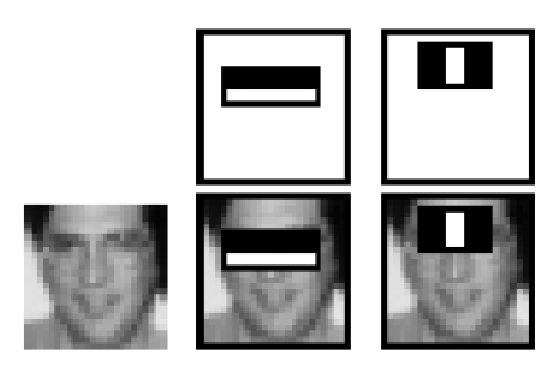
\includegraphics[scale=0.62]{eps/haar_features.eps}
			\caption{Esempi di feature rettangolari Haar.}
			\label{fig:haar_features}
		\end{figure}
		\begin{figure}[!htb]
			\centering
			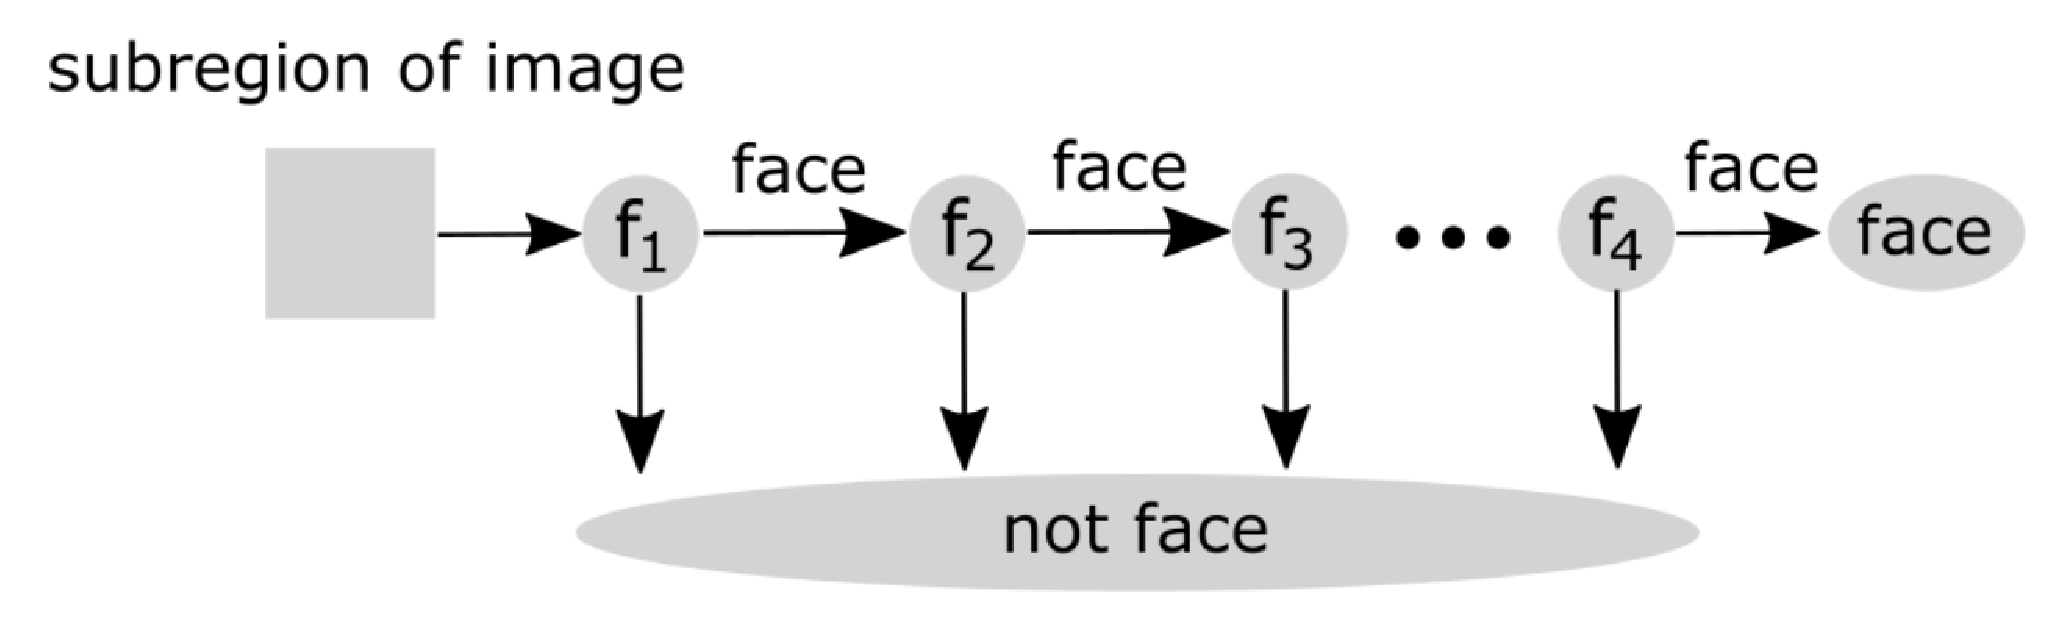
\includegraphics[scale=0.28]{eps/cascade_classifier.eps}
			\caption{Classificatore a cascata applicato\\alla localizzazione del volto.}
			\label{fig:cascade_classifier}
		\end{figure}
		\vspace{0.5cm}
		\item \textbf{LBP Cascade Classifier.}\\
		LBP\footnote{LBP. Local Binary Pattern.}\cite{Lbp1}\cite{Lbp2} è un classificatore che, come Haar, necessita di essere addestrato con centinaia di immagini.
		\begin{itemize}
			\item \textbf{Feature vector.}\\
			Ogni immagine di training è divisa in blocchi e per ogni blocco è adottata una finestra di 9 pixel (3x3), osservando con un particolare interesse il pixel collocato centralmente. Successivamente l'algoritmo compara il valore del pixel centrale con quello di ogni vicino all'interno della finestra 3x3. Ciascun pixel vicino con valore maggiore o uguale a quello del pixel centrale viene posto a 1, mentre i rimanenti a 0. In seguito, i valori dei pixel aggiornati sono letti in ordine orario, formando un numero binario. Tale numero binario viene poi convertito in notazione decimale e assegnato come nuovo valore per il pixel centrale. L'operazione (riassunta in Figura \ref{fig:lbp_block}) viene poi ripetuta per ogni pixel interno al blocco. Infine, i valori contenuti in ogni blocco sono convertiti in istogrammi. Concatenando essi si giunge a formare il vettore di feature per l'immagine che può essere utilizzato come descrittore di texture. Nell'ambito della localizzazione facciale si può osservare come ogni immagine di volto possa essere vista come una composizione di micro-pattern rilevabili effettivamente dall'operatore LBP, il quale è estendibile per la considerazione di rapporti di vicinanza differenti in raggio e numero. L'istogramma complessivo estratto modella la texture locale e la forma globale dei volti stessi. La Figura \ref{fig:lbp_histogram} ne riporta un esempio grafico. Le più importanti proprietà relativamente alle feature LBP si riferiscono alla loro tolleranza verso cambi di illuminazione e alla loro semplicità computazionale.
			\item \textbf{AdaBoost.}\\
			Un classificatore robusto è costruito utilizzando \textit{gentle AdaBoost} per rimuovere informazioni ridondanti dalle caratteristiche estratte.
			\item \textbf{Classificatore a cascata.}\\
			I classificatori a cascata sono formati dalle feature ottenute dall'algoritmo \textit{gentle AdaBoost}. Le sotto-regioni dell'immagine sono valutate a partire da un classificatore semplice sino ad arrivare a uno robusto. Se in qualunque stage il classificatore fallisce, la regione è scartata dalle iterazioni successive.
		\end{itemize}
		\vspace{0.5cm}
		\begin{figure}[!htb]
			\centering
			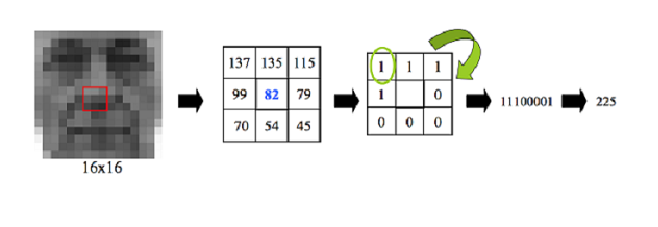
\includegraphics[scale=1]{eps/lbp_block.eps}
			\caption{Conversione LBP applicata a un blocco.}
			\label{fig:lbp_block}
		\end{figure}
		\begin{figure}[!htb]
			\centering
			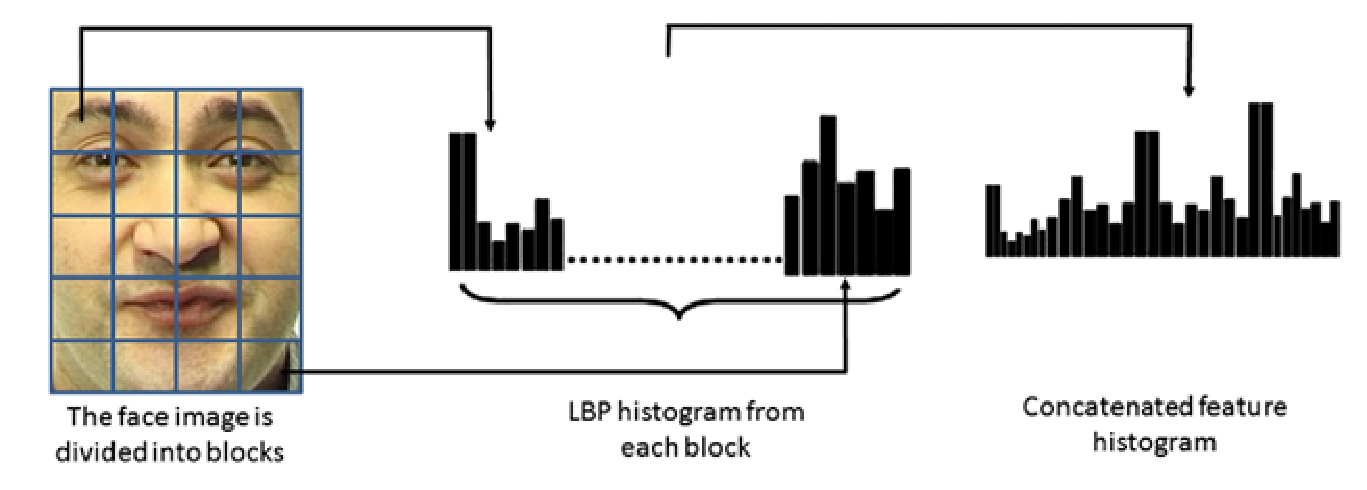
\includegraphics[scale=0.45]{eps/lbp_histogram.eps}
			\caption{Costruzione dell'istogramma rappresentante\\la feature LBP di un volto.}
			\label{fig:lbp_histogram}
		\end{figure}
		\vspace{0.5cm}
		\item \textbf{HOG + Linear SVM\footnote{SVM. Support Vector Machine.}.}\\
		L'idea base delle feature HOG\footnote{HOG. Histogram of Oriented Gradient.} è che la distribuzione dei gradienti di intensità locale o la direzione dei bordi possono caratterizzare bene l'aspetto e la forma di un oggetto o di un volto. L'algoritmo HOG conta le occorrenze dell'orientamento del gradiente in porzioni localizzate di un'immagine e si dimostra particolarmente utile per il riconoscimento di oggetti strutturati con parti deformabili. Similarmente a LBP, la rappresentazione dell'immagine è espressa come un istogramma combinato. Il metodo HOG è stato proposto per la prima volta da Navneet Dalal e Bill Triggs in un paper del 2005, dove venne dimostrato il suo uso abbinato con un SVM per l'addestramento di classificatori molto accurati\cite{Hog1}\cite{Hog2}.
		\item \textbf{Localizzatori basati su Deep learning.}\\
		Le CNN\footnote{CNN. Convolutional Neural Network.} costituiscono un approccio di deep learning in grado di realizzare il rilevamento facciale con un'accuratezza molto elevata, nonostante gli algoritmi richiedano un alto numero di dati per l'addestramento della rete neurale stessa. Secondariamente, localizzatori di questa tipologia necessitano di sistemi computazionali a elevate prestazioni per la costruzione del modello. Un'altra tecnica nota in letteratura per la localizzazione di volti, e in generale di oggetti, è SSD\footnote{SSD. Single Shot Detector.}.
	\end{itemize}
\end{itemize}

A seguito dello studio appena presentato (i cui risultati sono riassunti in Tabella \ref{table:face_detection}, specificatamente alla problematica del rilevamento del volto), si è scelto di non adottare algoritmi \textit{HOG + Linear SVM} o approcci basati su \textit{Deep learning}. Questa decisione deriva da un trade-off tra efficacia ed efficienza, inevitabile per via delle limitate capacità prestazionali di Raspberry Pi 3 B. Tecniche basate su HOG e Deep learning, infatti, nonostante siano ideali sul piano dell'accuratezza, non si dimostrano sufficientemente veloci per garantire le prestazioni real-time richieste dall'elaborato in esame. In fase di progettazione non si è inoltre operata una scelta ferma tra \textit{Haar Cascade Classifier} e \textit{LBP Cascade Classifier}, ritenendo opportuno testare entrambi gli algoritmi al fine di stabilire il migliore per la problematica trattata. È importante osservare tuttavia come si sia consapevoli - sin dalla fase di Design - dei limiti intrinseci del sistema in termini di risposta ai cambiamenti d'illuminazione, di efficacia con colorazioni scure della pelle e dall'eventuale uso di occhiali o oggettistica di altro tipo. Si nota infine come il limite nel riconoscimento di volti angolati non costituisca un problema di grande entità a causa della posizione frontale del volto assunta in larga parte da un conducente.

\begin{table}[h]
	\begin{adjustbox}{width=\textwidth}
	\begin{tabular}{|l|c|c|}
		\hline
		\multicolumn{1}{|c|}{\textbf{Algoritmo}} & \textbf{Vantaggi} & \textbf{Svantaggi}\\ \hline
		\textbf{Haar} &
		\begin{tabular}[c]{@{}c@{}}
			- Molto più veloce degli algoritmi\\
			HOG + Linear SVM
		\end{tabular} &
		\begin{tabular}[c]{@{}c@{}}
			- Meno accurato di HOG + Linear SVM\\
			- Produce un numero maggiore di\\falsi positivi
			rispetto a\\HOG + Linear SVM\\
			- Ha problemi nel riconoscimento\\di volti angolati
		\end{tabular}\\ \hline
		\textbf{LBP} &
		\begin{tabular}[c]{@{}c@{}}
			- Molto più veloce degli Haar cascade\\($\approx$ 3x)
		\end{tabular} &
		\begin{tabular}[c]{@{}c@{}}
			- Meno accurato degli Haar cascade
		\end{tabular}\\ \hline
		\textbf{HOG + Linear SVM} &
		\begin{tabular}[c]{@{}c@{}}
			- Significativamente più accurato\\degli Haar cascade\\
			- Produce un minor numero di falsi positivi\\rispetto agli Haar cascade
		\end{tabular} & - Più lento rispetto agli Haar cascade\\ \hline
		\textbf{Deep learning based} &
		\begin{tabular}[c]{@{}c@{}}
			- Significativamente più accurati e robusti\\di Haar e
			HOG + Linear SVM\\quando addestrati correttamente\\
			- Rilevano con buona accuratezza\\($\approx$ 70\%)
			anche volti angolati\\
			- Non hanno problemi con condizioni\\
			di luce critiche e ombre
		\end{tabular} &
		\begin{tabular}[c]{@{}c@{}}
			- Possono essere molto lenti\\sulla base della
			profondità e\\della complessità del modello\\
			- L'addestramento richiede molti dati
		\end{tabular}\\ \hline
	\end{tabular}
	\end{adjustbox}
	\caption{Comparazione tra i principali algoritmi di localizzazione del volto.}
	\label{table:face_detection}
\end{table}

\subsubsection{Rilevamento dei punti di riferimento facciali}
\label{subsubsec:facial_landmarks}

Dopo la localizzazione del volto (che da un punto di vista pratico fornisce il rettangolo all'interno del quale è collocato il viso del conducente), è applicato lo step di rilevamento degli occhi. Questo passaggio fornisce la base strutturale per la successiva estrazione di misure di sonnolenza. La localizzazione degli occhi è realizzata attraverso l'estrazione di \textit{facial landmark}. L'obiettivo è quello di individuare i punti di riferimento facciali di maggior importanza in ogni frame (es. occhi, naso, bocca, mento, sopracciglia), adottando metodi di previsione di forma (\textit{shape predictor}). Ciò è realizzato utilizzando una forma di mark-up consistente di diversi punti salienti, che viene adattata alla reale immagine del viso. Per stimare l'allineamento tra i punti del volto di mark-up e i punti di quello reale ci sono due principali categorie di approcci che possono essere adottati.
\begin{itemize}
	\item \textbf{Optimization-based}, che adattano la forma di mark-up in modo da ridurre al minimo una funzione di errore.
	\item \textbf{Regression-based}, che apprendono una funzione di regressione capace di realizzare direttamente l'associazione.
\end{itemize}
In questo progetto, la strategia di allineamento adottata consiste in una cascata di funzioni di regressione. Un'illustrazione della forma facciale di mark-up utilizzata è mostrata in Figura \ref{fig:facial_landmarks_68_markup}.

\begin{figure}[!htb]
	\centering
	\includegraphics[scale=0.12]{eps/facial_landmarks_68_markup.eps}
	\caption{Facial landmark mark-up a 68 punti.}
	\label{fig:facial_landmarks_68_markup}
\end{figure}

\subsubsection{Rilevamento della sonnolenza}

Per rilevare la sonnolenza, il progetto considera una misura comportamentale basata su una chiusura degli occhi protrattasi da parte del guidatore per un tempo superiore alla norma. Essere in grado di distinguere un occhio aperto da uno chiuso è di conseguenza fondamentale. A partire dai punti di riferimento facciali associati a un occhio è possibile applicare il calcolo dell'EAR, un'elegante metrica introdotta nel 2016 da \cite{EAR}.
Ogni occhio è rappresentato da 6 coordinate (x, y), enumerate a partire dal lato sinistro e proseguenti in ordine orario lungo la parte restante della regione (come riscontrabile in Figura \ref{fig:eye_6_landmarks}).
\begin{figure}[!htb]
	\centering
	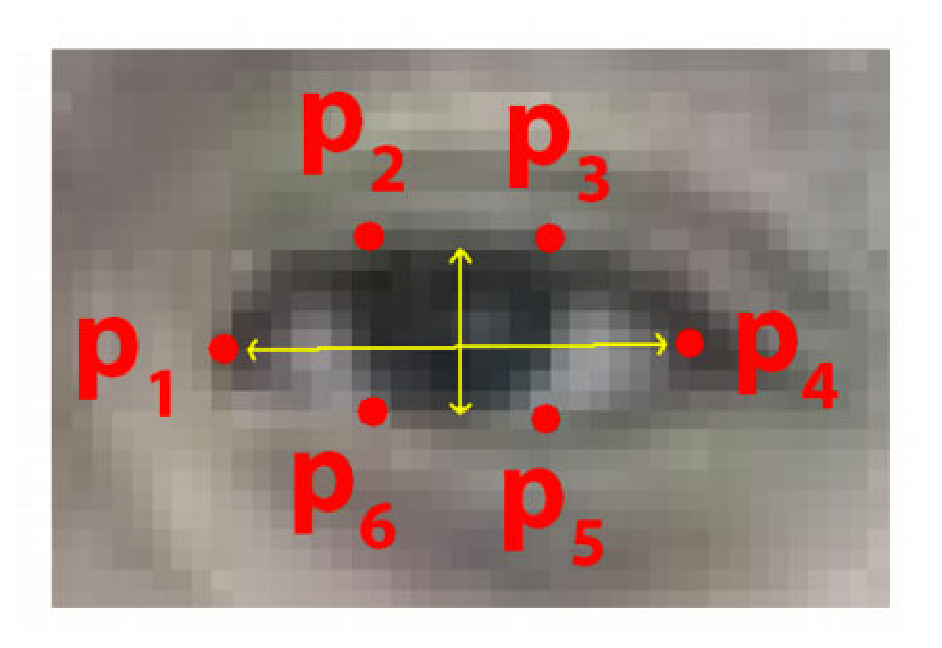
\includegraphics[scale=0.35]{eps/eye_6_landmarks.eps}
	\caption{I 6 punti di riferimento facciali associati a un occhio.}
	\label{fig:eye_6_landmarks}
\end{figure}
L'\textit{eye aspect ratio} esprime in forma di equazione una relazione tra la larghezza e l'altezza delle coordinate in oggetto.
\begin{equation}
EAR = \frac{\left\Vert{p_2 - p_6}\right\Vert + \left\Vert{p_3 - p_5}\right\Vert}{2 \times {\left\Vert{p_1 - p_4}\right\Vert}}
\end{equation}
Il numeratore dell'equazione computa la distanza tra i punti di riferimento verticali dell'occhio, mentre il denominatore considera la distanza tra i punti orizzontali (pesata opportunamente dal momento che vi sono un solo set di punti orizzontali e due set di punti verticali). La caratteristica che rende questa equazione interessante è legata al fatto che l'EAR assume un valore approssimativamente costante quando l'occhio è aperto, ma scende rapidamente a zero nel momento in cui lo si chiude. Questo approccio può pertanto essere usato sia per rilevare battiti di ciglia (\textit{eye blinking}) che per misurare il livello di apertura degli occhi. La Figura \ref{fig:blink_detection_plot} mostra l'andamento dell'EAR estratto da un video di esempio.
\begin{figure}[!htb]
	\centering
	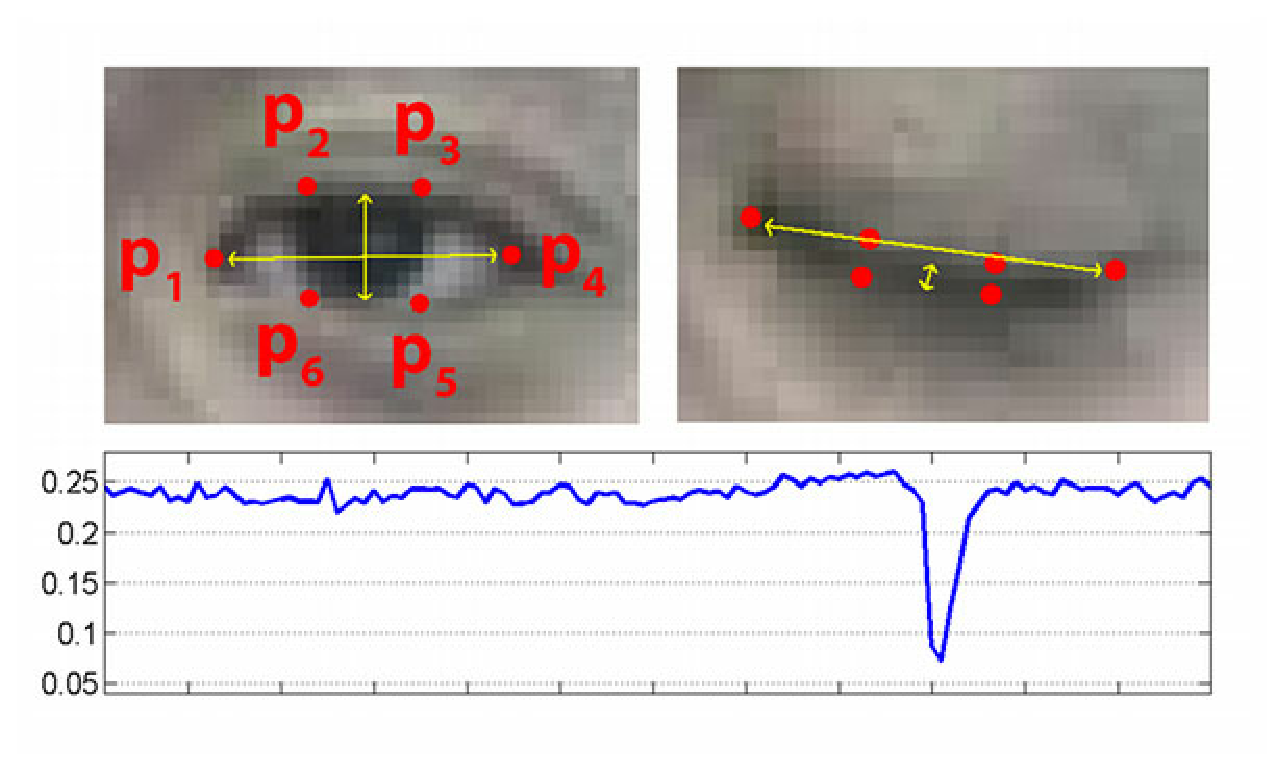
\includegraphics[scale=0.50]{eps/blink_detection_plot.eps}
	\caption{Esempio di segnale EAR lungo una sequenza video. Il brusco calo di valore e il suo successivo rialzo indica l'avvenimento di un battito di ciglia.}
	\label{fig:blink_detection_plot}
\end{figure}
I vantaggi derivanti dall'uso dell'EAR, nonché i motivi per cui si è scelto di basarsi su esso, sono:
\begin{itemize}
	\item consente di stimare l'apertura degli occhi mediante una sola grandezza scalare;
	\item nella sua versione base, è calcolabile da una sola immagine;
	\item ha una piccola varianza tra gli individui ed è completamente invariante rispetto a un ridimensionamento uniforme dell'immagine e alla rotazione in piano del viso;
	\item supera i risultati allo stato dell'arte su due dataset standard;
	\item è una semplice equazione calcolabile in breve tempo e capace di garantire un funzionamento real-time.
\end{itemize}
Queste caratteristiche rendono EAR una scelta ideale, tenendo conto anche dei limiti prestazionali di Raspberry Pi 3 B. Riepilogando, in fase di progettazione si è pertanto scelto di non far uso di metodi tradizionali di \textit{image processing} per il riconoscimento della chiusura degli occhi. Tali approcci (come \textit{template matching} o calcolo della percentuale di pixel interni alla regione bianca degli occhi) sono stati inizialmente presi in considerazione ma scartati in seguito, a causa della loro minor efficacia e del loro maggior costo da un punto di vista computazionale.\\
A partire dalla definizione di EAR, come indicato anche nel paper originario\cite{EAR}, tre metodi di classificazione possono essere adottati per il rilevamento della sonnolenza.
\begin{itemize}
	\item \textbf{EAR thresholding.}\\
	È fissato un valore di soglia e nel momento in cui l'EAR dell'utente diviene inferiore a essa per un determinato numero di frame consecutivi, una chiusura degli occhi è riconosciuta. Tuttavia, una singola soglia non è perfettamente adatta per tutte le persone dal momento che ogni individuo possiede il proprio \quotes{EAR naturale} in funzione delle caratteristiche facciali che lo contraddistinguono. Un approccio di questo tipo consente un'elaborazione per-frame ma tende a produrre un alto numero di falsi positivi. La discesa dell'EAR al di sotto della soglia, infatti, non necessariamente è dovuta a un \textit{eye blink} ma può essere provocata da espressioni facciali (es. parlato, sbadiglio o sorriso).
	\item \textbf{EAR SVM.}
	Si considera come input una finestra temporale più grande di un singolo frame (es. 13 frame consecutivi), cui associare uno stato dell'utente classificabile in tre categorie (occhio aperto, battito di ciglia, occhio chiuso). SVM è utilizzato come algoritmo di classificazione, definendo il problema come una funzione di mapping tra un vettore di input \texttt{x} e uno scalare di output \texttt{y} (0,1 o 2 sulla base della classe prevista). Un classificatore di questo tipo tuttavia possiede comunque diversi limiti e richiede un alto numero di dati eterogenei per l'addestramento. Inoltre è generale, ovvero è computato una volta sola e rimane lo stesso per tutti i dati di testing.
	\item \textbf{EAR HMM\footnote{HMM. Hidden Markov Model.}\cite{EarHmm}.} È un modello adattivo capace di far fronte alle principali problematiche dell'EAR SVM. L'EAR HMM, infatti, tiene conto di come la durata dei battiti di ciglia e la loro velocità differiscano da persona a persona (oltre che poter cambiare per lo stesso individuo nel tempo), rendendo l'EAR una caratteristica non statica. La Figura \ref{fig:ear_methods} ne riporta un'applicazione.  
\end{itemize}
Per il progetto in esame si è scelto di adottare EAR thresholding, a causa del ridotto tempo a disposizione (come requisito implementativo) e della non disponibilità di un elevato numero di dati etichettati specificatamente allo scenario di guida.
\begin{figure}[!htb]
	\centering
	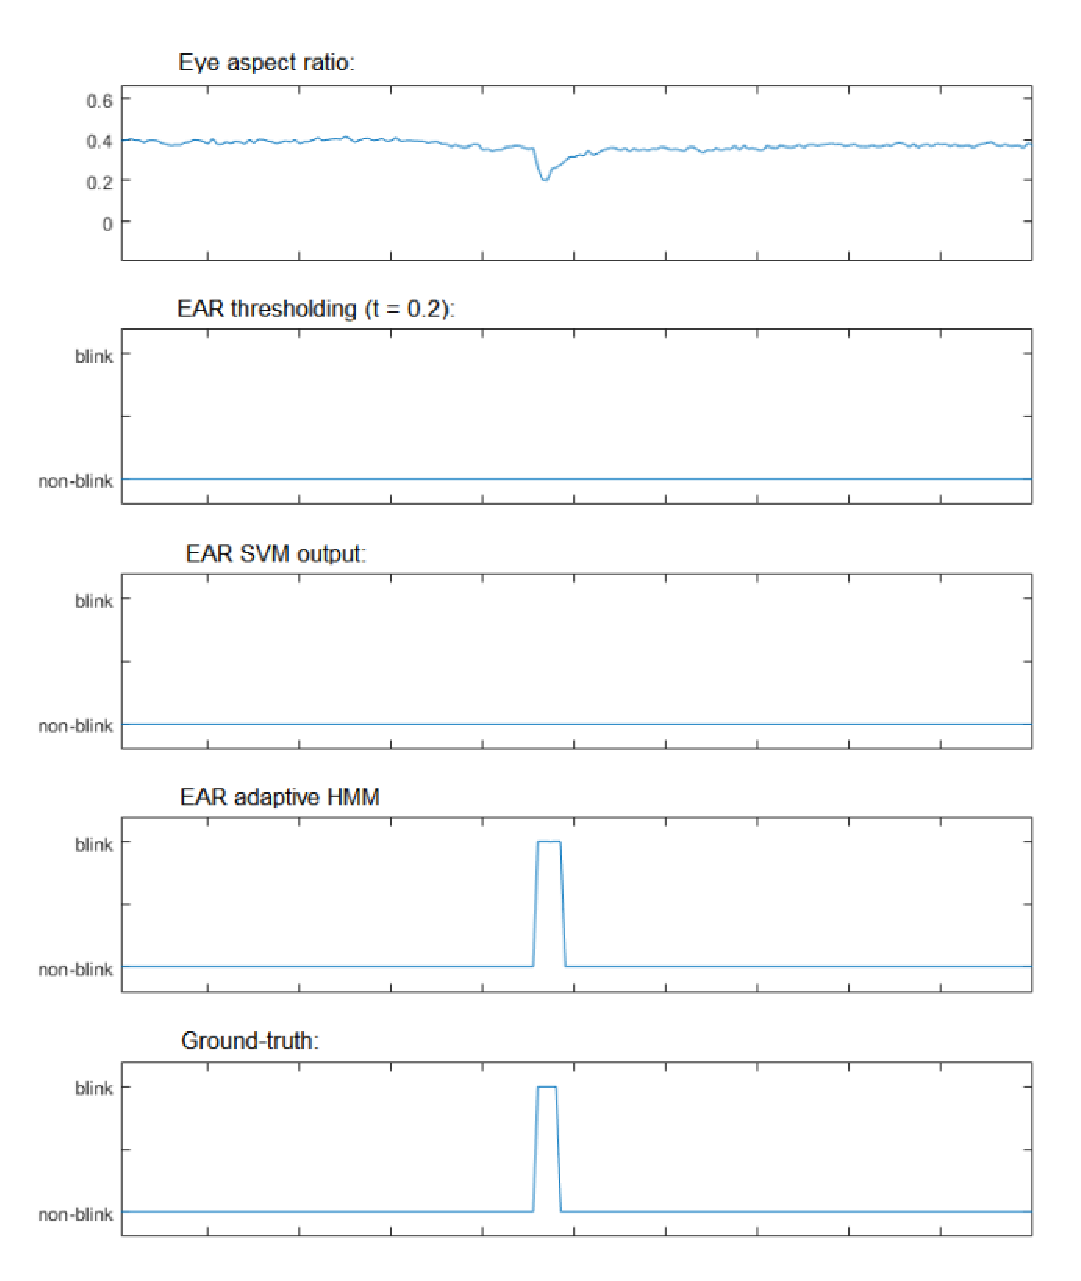
\includegraphics[scale=0.60]{eps/ear_methods.eps}
	\caption{Esempio di debole battito di ciglia. Solo il metodo adattivo EAR HMM è in grado di rilevarlo correttamente.}
	\label{fig:ear_methods}
\end{figure}

\subsection{Architettura software}
\label{subsec:software}

In Figura \ref{fig:flowchart} è riportato il flowchart illustrante l'esecuzione step-by-step (nelle sue parti principali) dell'algoritmo proposto, così come pensato in fase di progettazione.
\begin{figure}[!htb]
	\centering
	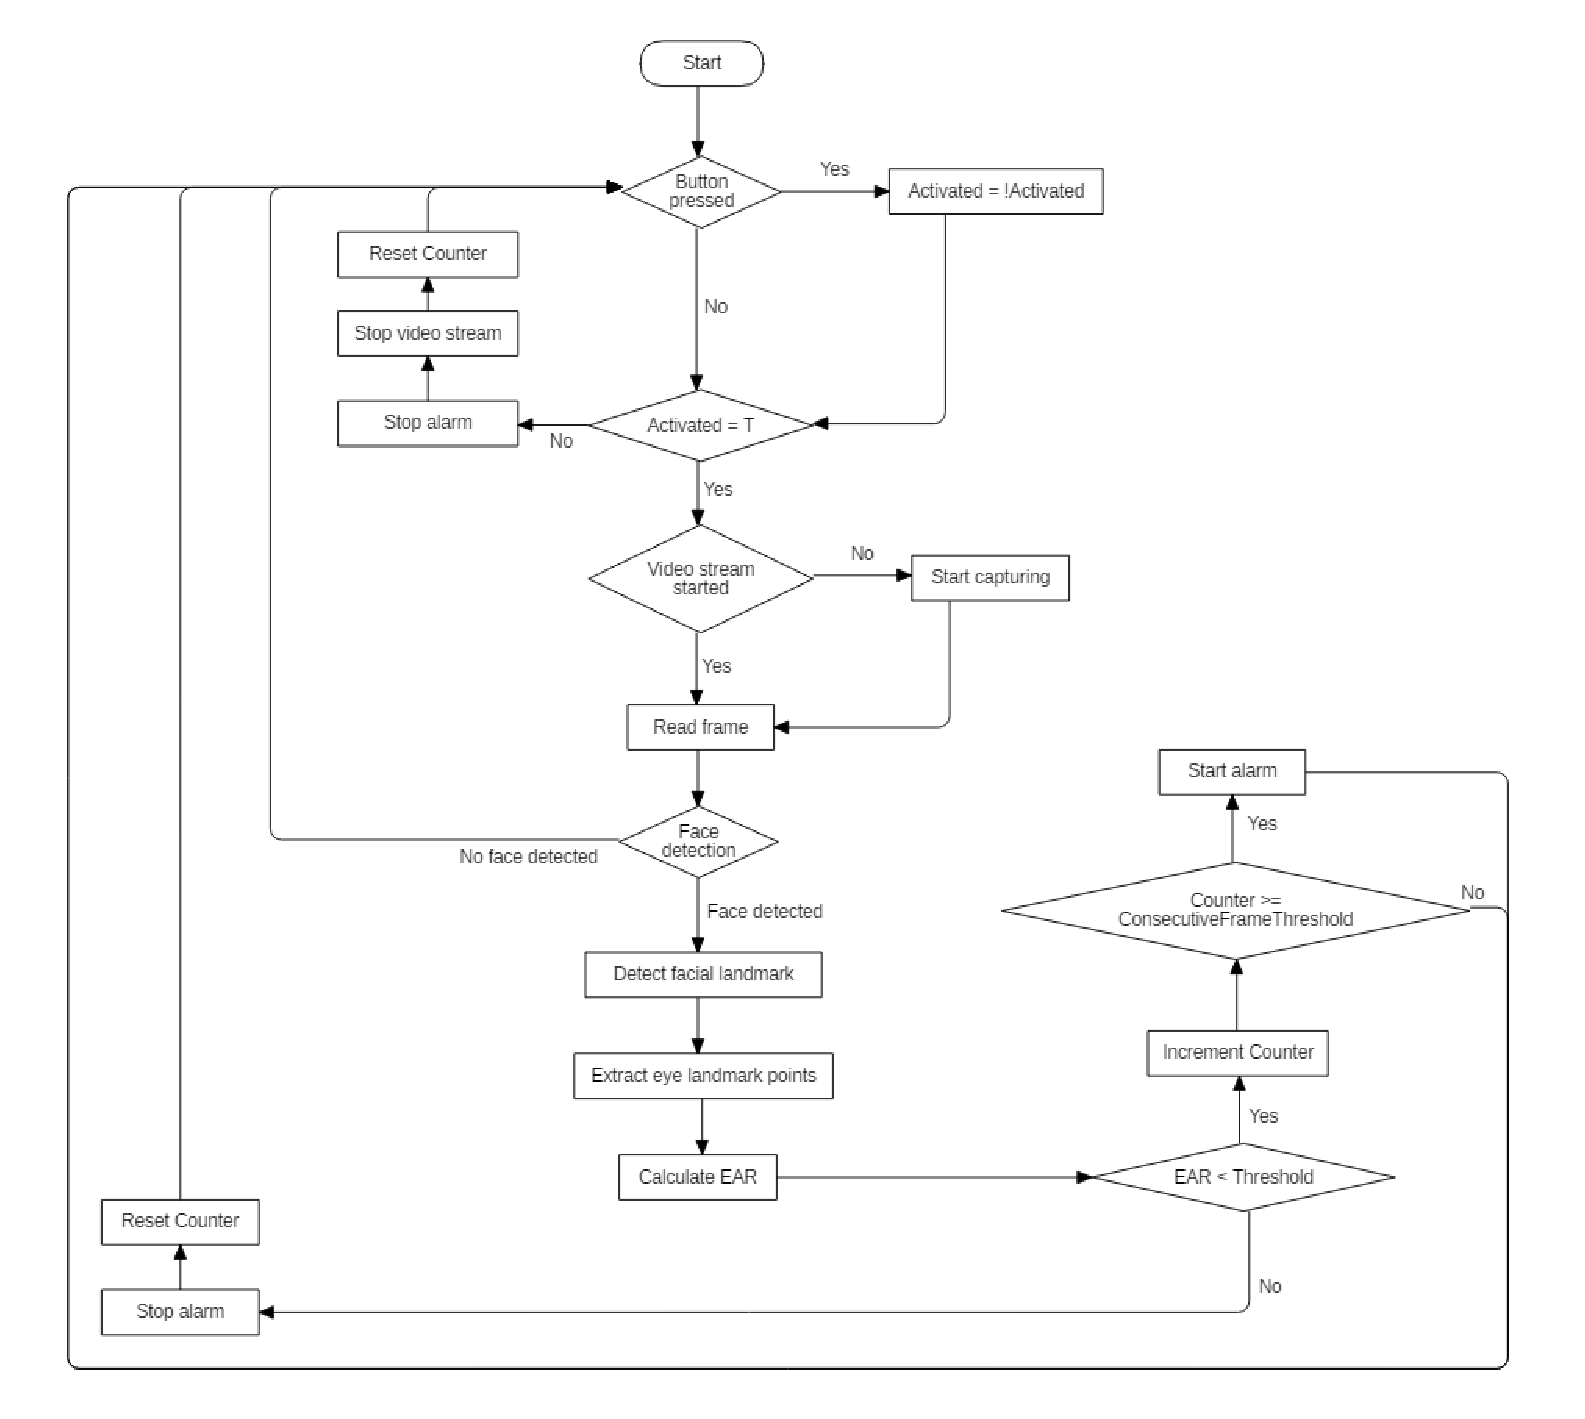
\includegraphics[scale=0.58]{eps/flowchart.eps}
	\caption{Flowchart dell'algoritmo.}
	\label{fig:flowchart}
\end{figure}
Il sistema è avviato con il boot di Raspberry Pi e, in seguito a questa fase, l'esecuzione del programma ha inizio automaticamente. Come già descritto nella sezione \ref{sec:requisiti}, l'accensione e lo spegnimento del rilevatore di sonnolenza è regolato mediante la pressione di un pulsante. Con l'attivazione del rilevatore, la camera (posizionata frontalmente al conducente) comincia la cattura dello stream video. Su ogni frame sono poi svolte delle operazioni di preprocessing per la successiva fase di localizzazione del volto. Se nessun volto è rilevato, l'algoritmo passa alla lettura del successivo frame (qualora il rilevatore risulti ancora attivo). In caso di rilevamento di un volto, invece, si procede all'individuazione dei punti di riferimento facciali all'interno della regione ottenuta (mediante \textit{shape predictor}). A partire dalle 12 coordinate estratte (6 per ogni occhio), si procede al calcolo dell'EAR. Se il valore dell'EAR risulta inferiore alla soglia fissata (il cui valore sarà stabilito dopo un'opportuna fase di test coinvolgente più utenti e scenari d'uso), gli occhi nel frame corrente sono considerati chiusi e un contatore viene incrementato. Quando gli occhi sono chiusi per un certo numero di frame consecutivi (il cui valore sarà sempre frutto di sperimentazioni finalizzate all'individuazione di una valida sensibilità), il conducente è ritenuto assonnato e l'allarme (sia visivo che sonoro) viene conseguentemente azionato. In ogni caso, si procede con l'analisi del successivo frame. Il contatore e l'allarme vengono sottoposti a reset solo nel caso in cui l'EAR calcolato non sia inferiore alla soglia (occhi aperti) o il pulsante per la disattivazione del rilevatore sia premuto dall'utente. In quest'ultimo caso viene anche arrestato lo streaming video dalla camera.

\subsection{Architettura fisica}
In Figura \ref{fig:circuit} è riportato lo schema circuitale.
\begin{figure}[!htb]
	\centering
	\includegraphics[scale=0.27]{eps/circuit.eps}
	\caption{Schema circuitale del progetto, disegnato con Fritzing\cite{Fritzing}.}
	\label{fig:circuit}
\end{figure}

I componenti hardware adottati per quanto concerne la costruzione del circuito sono:
\begin{itemize}
	\item 1 x Raspberry Pi 3 B
	\item 1 x RaspiCam v 1.3
	\item 1 x Buzzer attivo basso 3.3V-5V
	\item 1 x Pulsante tattile
	\item 3 x LED (1 verde, 1 giallo, 1 rosso)
	\item 3 x Resistenza 300$\Omega$
	\item 1 x Breadboard
	\item Cavetti di collegamento F-M e M-M
\end{itemize}

La camera board per Raspberry Pi è basata sul CMOS a colori OV5647, un sensore a 5MPixel con lenti 3.6mm F/2.0 fixed-focus in grado di fornire immagini con risoluzione massima di 2592x1944 e video 1080p30. Le dimensioni sono ridotte (21.6mm x 25mm) e la connessione avviene collegando il cavo flat al connettore CSI del Raspberry.

% MODE BCM

\iffalse

Devono essere esposte le scelte progettuali operate nelle varie fasi di sviluppo dell'elaborato.\\

In questa sezione devono essere documentati gli schemi di progetto relativamente all'architettura complessiva del sistema e alle sue componenti di rilievo che possano meritare un'analisi di dettaglio. Per le componenti software si può ricorrere ad esempio a diagrammi delle classi, di sequenza, stato, attività. Per le componenti hardware è possibile includere opportuni schemi in grado di descrivere l'architettura fisica adottata.\\

Vincoli circa la lunghezza della sezione (escluse didascalie, tabelle, testo nelle immagini, schemi):

\vspace{1cm}
\begin{tabular}{l|rr}
 & Numero minimo di battute & Numero massimo di battute \\
 \hline
 1 componente & 9000 & 18000 \\
 2 componenti & 12000 & 21000 \\
 3 componenti & 15000 & 24000 \\
 \hline
\end{tabular}
\fi

\newpage


%----------------------------------------------------------------------------------------
%	IMPLEMENTAZIONE
%----------------------------------------------------------------------------------------

\section{Implementazione}\label{sec:implementazione}

In questa sezione sono riportati i principali problemi affrontati durante l'effettiva realizzazione delle componenti hardware e software, illustrando le soluzioni implementative adottate.

\subsection{Configurazione Raspberry Pi}
Prima di essere utilizzato, il single-board computer Raspberry Pi dev'essere opportunamente configurato. Esso necessita, infatti, di un vero e proprio sistema operativo sul quale far affidamento. Solo successivamente, interagendo direttamente con esso, si è in grado di svolgere tutte le operazioni di progettazione, sviluppo e testing. L'intero procedimento di configurazione può essere suddiviso in due parti: la prima, incentrata sull'uso di un Personal Computer di appoggio e la seconda, direttamente realizzata sul dispositivo inizializzato.

\subsubsection{Memoria}
Tutto il software necessario per il corretto funzionamento del Raspberry è caricato in una scheda MicroSD, opportunamente tarata in termini di capacità per uno specifico progetto sulla base dell'occupazione di memoria richiesta da quest'ultimo. Considerando il prezzo contenuto e la semplice reperibilità di una scheda compatibile, si è preferito lasciare un modesto margine di memoria libera (adottandone una con capacità pari a 32GB), ampiamente sufficiente per contenere il sistema operativo, i vari IDE per lo sviluppo e l'intero dataset.

\subsubsection{Installazione Sistema Operativo}
In questa fase la MicroSD è connessa al Personal Computer, in modo che quest'ultimo possa essere utilizzato per configurarla. Prima di poter essere impiegata direttamente sul Raspberry, infatti, la scheda MicroSD dev'essere opportunamente formattata in formato FAT32. Per lo svolgimento di tale operazione si è fatto riferimento al software \quotes{SD Memory Card Formatter} (disponibile per Windows e Mac).

Successivamente occorre provvedere alla scelta del Sistema Operativo messo in esecuzione dal Raspberry. Questa decisione ricade sull'utente e sugli eventuali vincoli da soddisfare: esistono infatti numerose distro Linux disponibili gratuitamente al download e pronte all'utilizzo. Per quanto concerne il progetto in esame, seguendo le linee guida riportate direttamente sul sito del produttore, si è scelta la distribuzione \textit{Raspbian}: basata su Debian e opportunamente ottimizzata per funzionare su Raspberry Pi. Il caricamento di Raspbian, inoltre, può avvenire in due modi: attraverso l'operazione di \quotes{flash} del Sistema Operativo direttamente sulla MicroSD, oppure tramite un installer (denominato NOOBS\footnote{NOOBS. New Out Of the Box Software.}). Per facilità di installazione, si è preferita la seconda opzione: dopo l'ottenimento dell'archivio \textit{.zip} dal sito ufficiale, si è dunque estratto il suo contenuto direttamente dentro la MicroSD formattata in precedenza.

Giunti a questo punto, il dispositivo può avviare una modalità per l'installazione di tutti i componenti aggiuntivi desiderati. Soltanto al termine di questo passaggio la MicroSD può essere rimossa dal computer e inserita nell'apposito slot presente su Raspberry. Completata la procedura d'installazione guidata, grazie all'uso di alcune periferiche di input e output connesse direttamente al Raspberry Pi stesso (quali tastiera, mouse, monitor con entrata HDMI, cavo HDMI e alimentatore 5V / 2,1A), il device è pronto all'utilizzo e si può pertanto procedere alla seconda fase di configurazione.

\subsubsection{Installazione Software e Librerie}

Al termine della prima fase il Raspbery Pi è a tutti gli effetti un computer completo, dotato di browser, accesso a Internet (previa connessione via WiFi o Ethernet) e diversi software per lo sviluppo. Gli strumenti forniti di default non sono tuttavia sufficienti ai fini del progetto. Di conseguenza si procede all'installazione manuale di ulteriori pacchetti, tool e librerie al fine di consentire e agevolare il successivo sviluppo.

Prima di procedere con qualsiasi modifica, è buona norma assicurarsi che il pacchetto per l'ottenimento del software aggiuntivo sia aggiornato. Si eseguono due comandi per lo svolgimento di tale verifica:
\begin{lstlisting}
sudo apt-get update
sudo apt-get upgrade
\end{lstlisting}

Le seguenti fasi riportano il processo di installazione degli strumenti necessari per l'elaborato. L'ottemperanza dell'ordine proposto è importante per evitare il rischio di incorrere in dipendenze non sufficienti.\\

\textbf{Visual Studio Code}\\
È un editor di codice sorgente open source sviluppato da Microsoft, con supporto a diversi linguaggi di programmazione. Esso include il supporto a \textit{Syntax highlighting}, \textit{IntelliSense}, \textit{Snippet} e \textit{refactoring} del codice. Lo si ottiene, utilizzando la console, tramite due comandi:
\begin{lstlisting}
wget https://packagecloud.io/headmelted/codebuilds/gpgkey 
-O - | sudo apt-key add -
\end{lstlisting}
\begin{lstlisting}
curl -L https://code.headmelted.com/installers/apt.sh
| sudo bash
\end{lstlisting}

\vspace{0.5cm}
\textbf{OpenCV}\\
È una libreria software open source (discussa più approfonditamente nel successivo paragrafo \ref{subsec:opencv}).
Essa è disponibile in una versione ad hoc ottimizzata per dispositivi con ridotta capacità di calcolo, come Raspberry Pi. Per poterla utilizzare è necessario però installare alcune dipendenze, quali ad esempio \textit{libhdf5-dev}, \textit{libhdf5-serial-dev}, \textit{libqtwebkit4}, \textit{libqt4-test}, il package manager di Python e il gestore degli ambienti virtuali di Python. Le dipendenze in oggetto sono facilmente ottenibili tramite l'esecuzione di pochi comandi:
\begin{lstlisting}
sudo apt-get install libhdf5-dev libhdf5-serial-dev
sudo apt-get install libqtwebkit4 libqt4-test
sudo apt-get install build-essential cmake
sudo apt-get install libgtk-3-dev
sudo apt-get install libboost-all-dev
\end{lstlisting}
Lo stesso vale per il Package Manager di Python (\textit{pip}). È possibile ottenerlo mediante i comandi:
\begin{lstlisting}
wget https://bootstrap.pypa.io/get-pip.py
sudo python3 get-pip.py
\end{lstlisting}
Per poter lavorare comodamente con diversi progetti richiedenti librerie differenti, è preferibile utilizzare degli ambienti virtuali. Essi sono facilmente intercambiabili e permettono proprio di evitare conflitti di librerie nel caso in cui si vogliano gestire più progetti Python in un unico device. Utilizzando \textit{pip} si può facilmente ottenere il \quotes{Gestore degli Ambienti Virtuali}:
\begin{lstlisting}
pip install virtualenv virtualenvwrapper
\end{lstlisting}
Per utilizzare i comandi resi disponibili dal precedente pacchetto, occorre modificare il file \textit{~/.profile}, utilizzando un editor di testo a piacere (vim, nano o un tool grafico di qualunque natura) per inserire in coda le righe di seguito riportate.
\begin{lstlisting}
# virtualenv and virtualenvwrapper
export WORKON_HOME=$HOME/.virtualenvs
export VIRTUALENVWRAPPER_PYTHON=/usr/bin/python3
source /usr/local/bin/virtualenvwrapper.sh
\end{lstlisting}
Gli ambienti virtuali sono così pronti all'utilizzo, ma ogni qual volta che si apre una nuova finestra console è necessario eseguire il successivo comando per far riconoscere come valide le operazioni compiute per la gestione degli ambienti virtuali stessi.
\begin{lstlisting}
source ~/.profile
\end{lstlisting}
Per lo svolgimento del progetto si è creato un nuovo ambiente virtuale denominato \quotes{cv} grazie al comando:
\begin{lstlisting}
mkvirtualenv cv -p python3
\end{lstlisting}
Per impostare \quotes{cv} come ambiente di lavoro attuale, si è invece eseguito:
\begin{lstlisting}
workon cv
\end{lstlisting}
Tutte le librerie installate a fronte delle operazioni appena citate sono di conseguenza visibili esclusivamente nell'ambiente \quotes{cv}. Si procede dunque all'installazione di \textit{OpenCV} per Python:
\begin{lstlisting}
pip install opencv-contrib-python
\end{lstlisting}

\vspace{0.5cm}
\textbf{Imutils}\\
La procedura d'installazione della libreria \textit{imutils} (anch'essa descritta con maggior dettaglio nel paragrafo \ref{subsec:imutils}) è classica:
\begin{lstlisting}
pip install imutils
\end{lstlisting}

\vspace{0.5cm}
\textbf{Picamera}\\
È una libreria di appoggio per l'uso della RaspiCam direttamente in Python, installabile tramite il seguente comando:
\begin{lstlisting}
pip install "picamera[array]"
\end{lstlisting}
Sempre in riferimento a RaspiCam, Raspberry mette a disposizione due programmi per il testing della camera: \texttt{raspistill} (per immagini singole) e \texttt{raspivid} (per i video). Un test di acquisizione può essere fatto semplicemente con:
\begin{lstlisting}
raspistill -o image.jpg
\end{lstlisting}

\vspace{0.5cm}
\textbf{Dlib}\\
Un'ulteriore libreria utilizzata nel progetto è \textit{Dlib} (paragrafo \ref{subsec:dlib}); per essere pienamente operativa, essa ha prima bisogno di alcune dipendenze, reperibili tramite i seguenti comandi (lanciati \underline{fuori} dall'ambiente virtuale di python):
\begin{lstlisting}
sudo apt-get install build-essential cmake
sudo apt-get install libgtk-3-dev
sudo apt-get install libboost-all-dev
\end{lstlisting}
Le ulteriori dipendenze e la libreria \textit{Dlib} stessa sono reperibili grazie all'utilizzo di \textit{pip}. Per eseguire questi comandi è necessario trovarsi nell'ambiente virtuale di Python precedentemente creato.
\begin{lstlisting}
pip install numpy
pip install scipy
pip install scikit-image
\end{lstlisting}

\vspace{0.5cm}
Prima di procedere allo sviluppo vero e proprio del progetto, è consigliabile testare le librerie appena installate. Senza chiudere la finestra precedentemente aperta (oppure aprendone una nuova e rieseguendo i comandi per il cambio di ambiente virtuale) si possono eseguire in ordine i comandi:
\begin{lstlisting}
python
import cv2
import imutils
\end{lstlisting}
L'assenza di errori restituiti indica un'installazione avvenuta con successo. Se così non fosse, si può procedere all'integrazione di alcune librerie probabilmente mancanti oppure provare a ripetere l'installazione su un nuovo ambiente virtuale.

\subsubsection{Ottimizzazione Utilizzo Risorse}

Il progetto presenta numerose e complesse elaborazioni su immagini. Avendo a disposizione un buon margine di memoria sulla MicroSD è consigliabile incrementare virtualmente la quantità della RAM disponibile, modificando opportunamente l'attuale configurazione del sistema. Uno dei modi per riservare una parte dello spazio presente sulla scheda ai fini dell'elaborazione è quello di incrementare la dimensione dello \quotes{swap file}. Questo può essere fatto lanciando come amministratore il comando:
\begin{lstlisting}
sudo nano /etc/dphys-swapfile
\end{lstlisting}
e sostituendo alla stringa \quotes{CONF\_SWAPSIZE} il valore che si desidera assegnare al file di swap stesso (espresso in megabyte). Nel progetto in questione si è scelto di dedicare un ulteriore gigabyte di spazio:
\begin{lstlisting}
CONF_SWAPSIZE=1024
\end{lstlisting}
Un altro cambiamento alle impostazioni - utile a incrementare le performance e a ricavare qualche megabyte di memoria - riguarda la diminuzione della RAM riservata ai calcoli della GPU. Ciò è possibile dal momento che tutte le elaborazioni necessarie si svolgono proprio sulla CPU. Si può pertanto personalizzare tale parametro attraverso il menù dedicato alla configurazione del Raspberry, accessibile grazie al comando
\begin{lstlisting}
raspi-config
\end{lstlisting}
sotto la categoria \quotes{Advanced Options $\rightarrow$ Memory Split}. La dimensione impostata per questo progetto è stata di 16MB: quantità di memoria più che sufficiente per riuscire ad avviare il Raspberry anche in modalità desktop grafico. Per rendere operative le suddette modifiche, infine, è necessario eseguire il reboot.

\subsection{Tecnologie}

\subsubsection{Python}
Python è utilizzato come principale linguaggio di programmazione. Esso, nello specifico, è un linguaggio object-oriented, creato da Guido Rossum nel 1989 e progettato per una rapida prototipazione di applicazioni complesse. È in grado di interfacciarsi con molte chiamate di sistema e librerie (tra cui anche OpenCV e Dlib), ed è estendibile al C o al C++. Python è inoltre molto utilizzato in discipline quali \textit{Artificial Intelligence}, \textit{Data Mining}, \textit{Machine Learning} e altri campi avanzati della Computer Science. È stato scelto per l'importanza da esso attribuita alla leggibilità dal codice e per la sua compatibilità cross-platform. Python è anche il linguaggio maggiormente consigliato per uno sviluppo su Raspberry Pi, tra quelli supportati.

\subsubsection{OpenCV}
\label{subsec:opencv}
OpenCV\cite{OpenCV} è una libreria multipiattaforma di Computer Vision open source originariamente sviluppata da Intel, progettata per essere computazionalmente efficiente e utilizzabile da applicazioni real time. Essa consente di velocizzare e di semplificare lo sviluppo di applicazioni di visione. La struttura di OpenCV consta di 6 parti: CXCORE (strutture dati), CV (funzioni per il processing e analisi di immagini, calibrazione e pattern recognition), ML (machine learning), HighGUI (interfacce utenti), CVCAM (interfacce webcam) e CVAUX (algoritmi sperimentali). Nell'ambito dell'elaborato, è stata utilizzata per eseguire automaticamente l'operazione di \textit{face detection} (a partire dal caricamento della conoscenza in un classificatore a cascata), per elaborare efficientemente i frame acquisiti dalla camera con prestazioni real time e per visualizzare in output i risultati calcolati. La scelta legata all'uso di OpenCV, in conclusione, deriva dalla sua completezza e convenienza.

\subsubsection{Dlib}
\label{subsec:dlib}
Dlib\cite{Dlib} è un moderno toolkit C++ che contiene algoritmi e strumenti di machine learning per creare software complessi al fine di risolvere problemi del mondo reale. È utilizzato sia nell'industria che nel mondo accademico in una vasta gamma di domini, tra cui la robotica, i dispositivi embedded, i telefoni cellulari e gli ambienti di elaborazione ad alte prestazioni e di grandi dimensioni. La licenza open source di Dlib consente di utilizzarlo in qualsiasi applicazione, gratuitamente.\\
Relativamente all'elaborato, la libreria Dlib è stata scelta in quanto fornisce uno \textit{shape predictor}\cite{DlibShapePredictor} - già addestrato e altamente ottimizzato - basato su una rete neurale e facente uso di HOG + SVM nella procedura. Tale \textit{shape predictor} implementa la strategia di allineamento con funzioni di regressione in cascata (già citata nella sezione \ref{subsubsec:facial_landmarks}) ed è utilizzabile per l'individuazione di \textit{facial landmark} a 68 punti (da cui procedere per il calcolo dell'EAR).

\subsubsection{Imutils}
\label{subsec:imutils}
Imutils\cite{Imutils} è una libreria open source mantenuta dalla community di \textit{pyimagesearch}\cite{Pyimagesearch} (noto blog dedicato alla Computer Vision e realizzato da Adrian Rosebrock). Essa contiene una serie di funzioni di utilità per l'elaborazione di immagini (come traslazione, rotazione, ridimensionamento) finalizzate a semplificare il lavoro con OpenCV e Python. All'interno dell'elaborato è stata utilizzata per leggere i frame catturati dalla RaspiCam (\textit{VideoStream}), per semplificare l'accesso ai landmark degli occhi restituiti da Dlib, per compiere operazioni di resizing con mantenimento dell'aspect ratio e per calcolare la velocità dell'algoritmo in termini di FPS.

\subsection{Real time drowsiness detection script}
\label{subsec:main_script}
Di seguito si riportano le porzioni di codice ritenute maggiormente significative per lo script Python dedicato al rilevamento real time della sonnolenza durante la guida.\\
Al fine di poter cambiare agilmente i parametri principali dell'algoritmo, si è scelto di specificare quest'ultimi come argomenti a linea di comando. Lo script, in particolare, ne richiede due obbligatori e uno opzionale.
\begin{itemize}
	\item \texttt{--cascade} (obbligatorio), si riferisce al file XML contenente la conoscenza del classificatore a cascata che si vuole utilizzare per la localizzazione del volto. Così facendo è possibile passare rapidamente da un'operazione di \textit{face detection} basata su Haar feature a una realizzata con LBP (per le ragioni già illustrate nel paragrafo \ref{subsubsec:face_detection} della precedente sezione).
	\item \texttt{--shape-predictor} (obbligatorio), è il percorso al file .dat per la costruzione dello shape predictor di Dlib per l'individuazione dei \textit{facial landmark}.
	\item \texttt{--alarm} (opzionale), indica se il buzzer acustico debba essere utilizzato o meno in caso di rilevamento di sonnolenza.
\end{itemize}

\begin{python}
	ap = argparse.ArgumentParser()
	ap.add_argument("-c", "--cascade", required=True,
		help = "path to where the face cascade resides")
	ap.add_argument("-p", "--shape-predictor", required=True,
		help="path to facial landmark predictor")
	ap.add_argument("-a", "--alarm", type=int, default=0,
		help="boolean used to indicate if buzzer should be used")
	args = vars(ap.parse_args())
\end{python}

\vspace{0.3cm}
Dopo aver letto i parametri di input, si procede con la configurazione dei pin di GPIO per i tre LED (output) e per il buzzer (input). Tale operazione, data la sua semplicità, non è riportata all'interno della relazione. A seguito del setup dei pin stessi, si effettua il caricamento della conoscenza per il riconoscimento del volto all'interno del tipo \texttt{CascadeClassifier} di OpenCV (pensato generalmente per la localizzazione di oggetti)\cite{OpenCVCascadeClassifier}. Successivamente si crea anche l'oggetto \textit{predictor} di Dlib, sempre a partire dal path indicato come argomento al lancio dello script.
\vspace{0.3cm}

\begin{python}
	# load OpenCV's Haar/LBP cascade for face detection (which
	# is faster than dlib's built-in HOG detector, but less
	# accurate), then create the facial landmark predictor
	detector = cv2.CascadeClassifier(args["cascade"])
	predictor = dlib.shape_predictor(args["shape_predictor"])
\end{python}

\vspace{0.3cm}
I \textit{facial landmark} prodotti da Dlib sono racchiusi in una lista di 64 elementi (uno per ogni coordinata significativa del volto). Per accedere alle regioni degli occhi si fa uso della libreria \textit{imutils}, che fornisce la possibilità di ottenere gli indici corretti (\textit{array slice}) della regione d'interesse interna alla \quotes{shape} semplicemente mediante un accesso associativo facente uso del nome come chiave.
\vspace{0.3cm}

\begin{python}
	# grab the indexes of the facial landmarks for the left and
	# right eye, respectively
	(lStart, lEnd) = face_utils.FACIAL_LANDMARKS_IDXS["left_eye"]
	(rStart, rEnd) = face_utils.FACIAL_LANDMARKS_IDXS["right_eye"]
\end{python}

\vspace{0.3cm}
A fronte dell'attivazione del rilevatore mediante la pressione del pulsante (vedi sezione \ref{sec:requisiti}), è necessario avviare lo stream video dalla RaspiCam su un nuovo thread. A tal scopo si è nuovamente fatto uso di una classe interna a \textit{imutils}: \texttt{VideoStream}. L'attesa di un secondo consente al sensore di camera di riscaldarsi.
\vspace{0.3cm}

\begin{python}
	vs = VideoStream(usePiCamera=True).start()
	time.sleep(1.0)
\end{python}

\vspace{0.3cm}
Giunti a questo punto si esegue la lettura ciclica dei frame catturati dallo stream. Prima di passare alla localizzazione del volto, ogni frame viene ridimensionato a una larghezza di 450 pixel (utilizzando la funzione fornita da \textit{imutils}, per i vantaggi posseduti rispetto a quella standard di OpenCV) e convertito in scala di grigi. Queste trasformazioni riducono la dimensione del frame e rendono pertanto il successivo processo di rilevazione sensibilmente più efficiente. L'individuazione dei volti contenuti nell'immagine grayscale è invece  realizzata grazie al metodo OpenCV \texttt{detectMultiScale}\cite{OpenCVCascadeClassifier}.
\vspace{0.3cm}

\begin{python}
	# grab the frame from the threaded video file stream, resize
	# it, and convert it to grayscale channels)
	frame = vs.read()
	frame = imutils.resize(frame, width=450)
	gray = cv2.cvtColor(frame, cv2.COLOR_BGR2GRAY)
	
	# detect faces in the grayscale frame
	rects = detector.detectMultiScale(gray, scaleFactor=1.1, 
		minNeighbors=5, minSize=(30, 30),
		flags=cv2.CASCADE_SCALE_IMAGE)
\end{python}

\vspace{0.3cm}
Per ogni volto rilevato col classificatore a cascata specificato in input, OpenCV restituisce un rettangolo corrispondente al \textit{bounding box} del volto stesso. Le coordinate di questo oggetto sono usate per la costruzione di un \texttt{dlib.rectangle}. Grazie a esso è possibile avviare la predizione dei \textit{facial landmark} sulla sola regione dell'immagine contenente il volto individuato con l'algoritmo di localizzazione. La \quotes{shape} restituita da Dlib - formata da coordinate (x, y) - è poi convertita in un \textit{NumPy array} da cui possono essere estratte le 12 coordinate degli occhi. Inoltre, è importante osservare che l'estrazione dei punti di riferimento facciali non è nemmeno perseguita nel caso in cui non venga individuato nessun volto all'interno del frame.
\vspace{0.3cm}

\begin{python}
	# loop over the face detections
	for (x, y, w, h) in rects:
		# construct a dlib rectangle object from the Haar cascade
		# bounding box
		rect = dlib.rectangle(int(x), int(y), int(x + w),
		int(y + h))
		
		# determine the facial landmarks for the face region, then
		# convert the facial landmark (x, y)-coordinates to a NumPy
		# array
		shape = predictor(gray, rect)
		shape = face_utils.shape_to_np(shape)
		
		# extract the left and right eye coordinates, then use the
		# coordinates to compute the eye aspect ratio for both eyes
		leftEye = shape[lStart:lEnd]
		rightEye = shape[rStart:rEnd]
		...
\end{python}

\vspace{0.3cm}
A partire dalle coordinate di ogni occhio è possibile calcolare l'EAR. Si sono così implementate due funzioni: una per il calcolo della distanza euclidea tra due punti (incentrata su \textit{NumPy}) e l'altra per l'elaborazione dell'\textit{Eye Aspect Ratio} vero e proprio. Per offrire una stima dell'apertura di entrambi gli occhi e non di uno soltanto, si è scelto di calcolare il valore di EAR medio (come indicato nel paper originario\cite{EAR}).
\vspace{0.3cm}

\begin{python}
	def euclidean_dist(ptA, ptB):
		# compute and return the euclidean distance between the two
		# points
		return np.linalg.norm(ptA - ptB)
	
	def eye_aspect_ratio(eye):
		# compute the euclidean distances between the two sets of
		# vertical eye landmarks (x, y)-coordinates
		A = euclidean_dist(eye[1], eye[5])
		B = euclidean_dist(eye[2], eye[4])
		
		# compute the euclidean distance between the horizontal
		# eye landmark (x, y)-coordinates
		C = euclidean_dist(eye[0], eye[3])
		
		# compute the eye aspect ratio
		ear = (A + B) / (2.0 * C)
		
		# return the eye aspect ratio
		return ear
\end{python}

\vspace{0.3cm}
Calcolato l'EAR si prosegue con la sua comparazione rispetto al valore di soglia fissato ($EAR_{th}$), seguendo il procedimento già evidenziato col flowchart del precedente paragrafo \ref{subsec:software}. Per ragioni di visualizzazione, si cita l'uso di \texttt{cv2.imshow}: tramite esso si sono mostrati i frame elaborati, disegnando su ciascuno di questi (tramite \texttt{cv2.putText}, \texttt{cv2.drawContours} e \texttt{cv2.rectangle}) i valori di EAR, il conteggio di frame, il \textit{bounding box} del volto, le regioni associate agli occhi e gli avvisi di sonnolenza. La Figura \ref{fig:drowsiness_output} mostra un esempio di tale output.

\begin{figure}
	\begin{subfigure}{.5\textwidth}
		\centering
		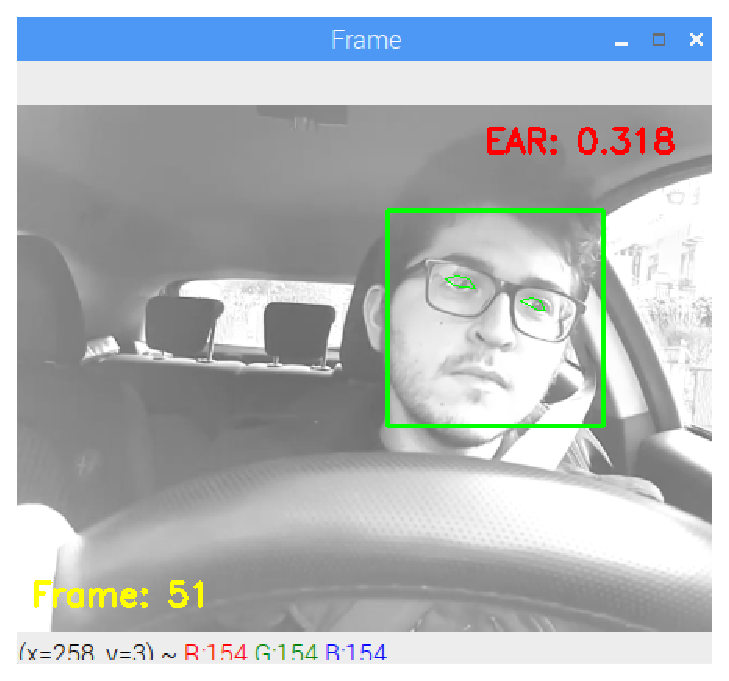
\includegraphics[width=.8\linewidth]{eps/gf_opened_eyes.eps}
		\caption{Output con guidatore sveglio.}
	\end{subfigure}
	\hspace{5mm}
	\begin{subfigure}{.5\textwidth}
		\centering
		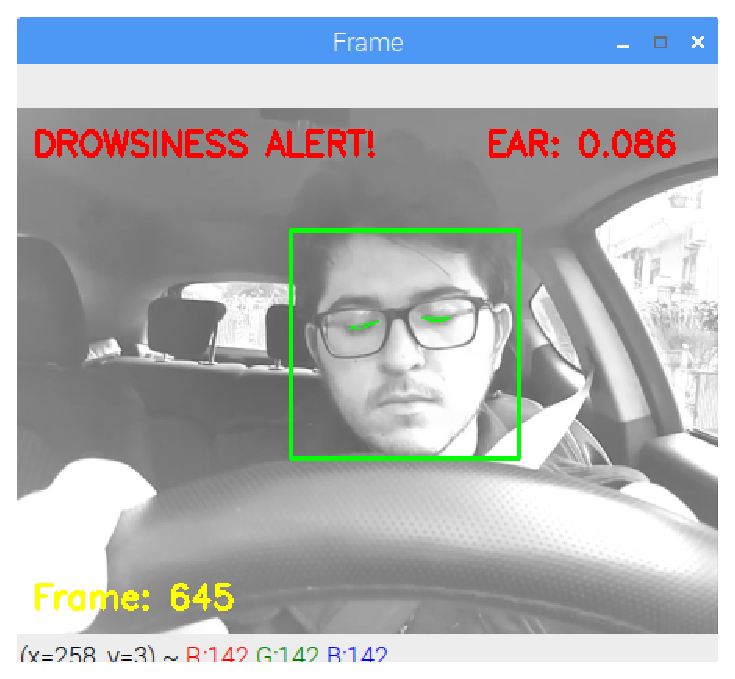
\includegraphics[width=.8\linewidth]{eps/gf_closed_eyes.eps}
		\caption{Output con guidatore assonnato.}
	\end{subfigure}
	\caption{Output grafico fornito da \texttt{drowsiness\_stream\_detector.py}.}
	\label{fig:drowsiness_output}
\end{figure}

\subsection{Lancio dello script in fase di reboot}
% TO DO
a\\
b\\
c\\
d\\
f\\
g\\
h\\


\iffalse
Esporre i principali problemi affrontati durante l'effettiva realizzazione delle componenti hardware/software e illustrare le soluzioni implementative adottate. Se l'elaborato ha previsto l'utilizzo di tecnologie già disponibili sul mercato, discuterne brevemente le caratteristiche e motivarne l'adozione rispetto ad altre soluzioni assimilabili.\\

\textbf{NOTA: in questa sezione devono essere riportate esclusivamente le porzioni di codice ritenute particolarmente significative. Il codice sorgente nella sua interezza, opportunamente commentato, deve essere consegnato separatamente dalla relazione in un archivio compresso.}\\

Vincoli circa la lunghezza della sezione (escluse didascalie, tabelle, testo nelle immagini, schemi):

\vspace{1cm}
\begin{tabular}{l|rr}
& Numero minimo di battute & Numero massimo di battute \\
\hline
1 componente & 5000 & 11000 \\
2 componenti & 8000 & 16000 \\
3 componenti & 10000 & 21000 \\
\hline
\end{tabular}
\fi

\newpage


%----------------------------------------------------------------------------------------
%	TESTING E PERFORMANCE
%----------------------------------------------------------------------------------------

\section{Testing e performance}

\subsection{LBP VS Haar}
A seguito dell'implementazione, lo script \texttt{drowsiness\_stream\_detector.py} - illustrato nel paragrafo \ref{subsec:main_script} -  è stato da subito testato sia con conoscenza LBP che Haar (\texttt{--cascade}), mettendo a confronto i risultati. Durante lo svolgimento di questa fase è emerso come un classificatore LBP sia effettivamente più veloce di Haar (11 FPS anzichè 7) ma anche sensibilmente meno accurato, confermando quanto noto in letteratura (paragrafo \ref{subsubsec:face_detection}). A fronte del ridotto dislivello prestazionale, si è ritenuto opportuno preferire gli Haar Cascade Classifier per il loro maggior numero di localizzazioni con successo. Considerando come la durata media di un battito di ciglia si attesti tra i 300 e i 400 millisecondi, si è scelto di fissare il numero necessario di frame consecutivi con EAR sotto la soglia per l'instaurazione dell'allarme a 16 (dimostratosi essere un valore adatto dal punto di vista della sensibilità).

\subsubsection{Limiti di Haar}
Nella conduzione delle prove sperimentali si ha avuto modo di verificare alcuni limiti di Haar Cascade Classifier nella localizzazione facciale. Nonostante sia perfettamente in grado di individuare volti orientati frontalmente rispetto alla camera o leggermente angolati, infatti, l'algoritmo non si è dimostrato capace di far fronte a inclinazioni della testa o ad angolazioni più marcate. La Figura \ref{fig:face_poses} ne riporta alcuni esempi pratici.

\begin{figure}[!htb]
	\begin{subfigure}{.3\textwidth}
		\centering
		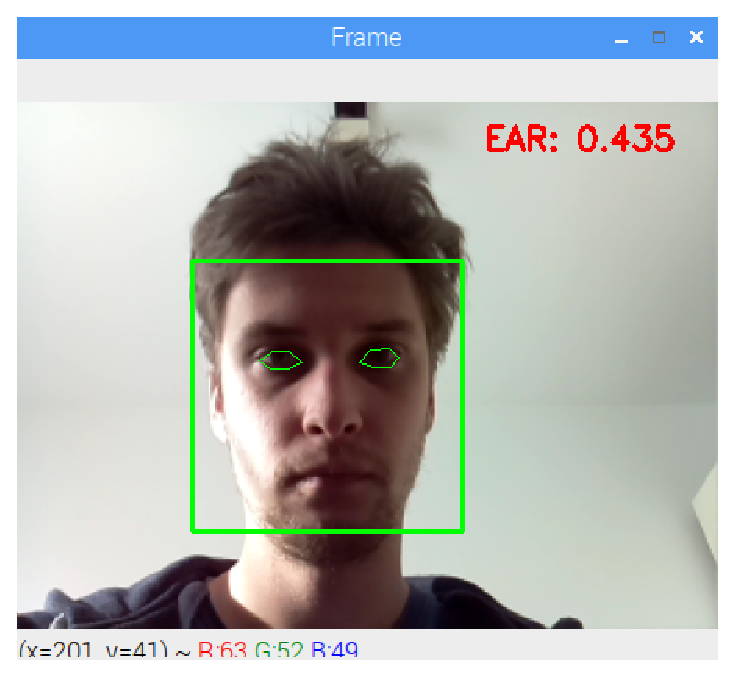
\includegraphics[width=.8\linewidth]{eps/mp_straight_view.eps}
		\caption{Volto in posizione frontale.}
	\end{subfigure}
	\hspace{5mm}
	\begin{subfigure}{.3\textwidth}
		\centering
		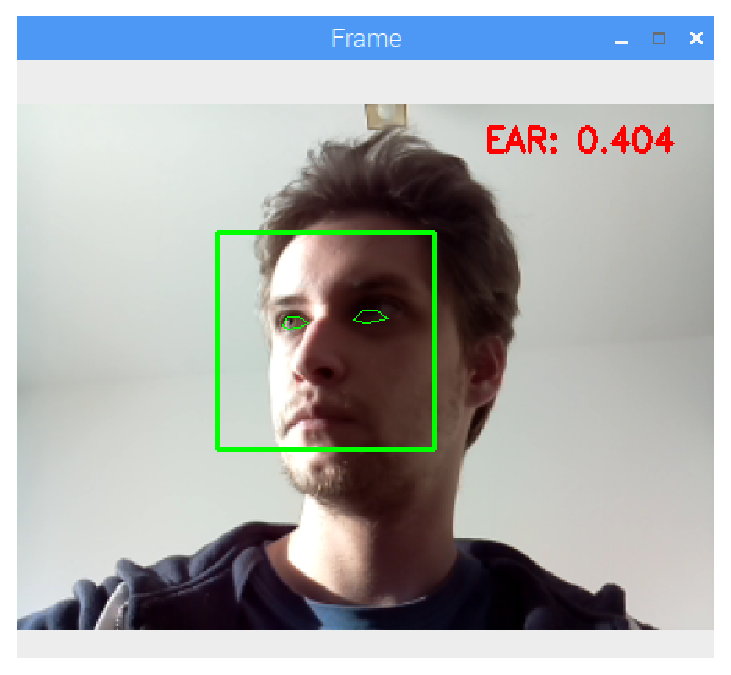
\includegraphics[width=.8\linewidth]{eps/mp_right_view.eps}
		\caption{Volto parzialmente rivolto a destra.}
	\end{subfigure}
	\hspace{5mm}
	\begin{subfigure}{.3\textwidth}
		\centering
		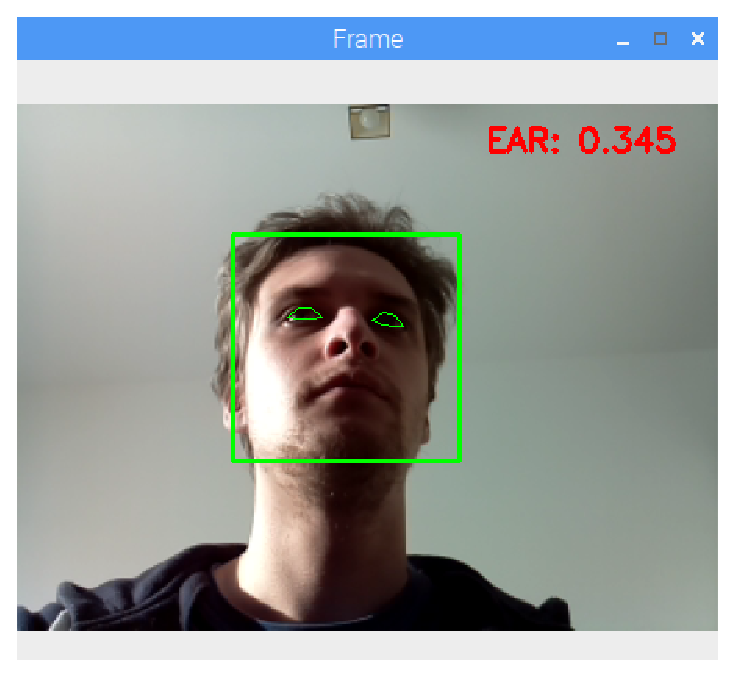
\includegraphics[width=.8\linewidth]{eps/mp_upward_view.eps}
		\caption{Volto rivolto verso l'alto.}
	\end{subfigure}
	\par\bigskip % force a bit of vertical whitespace
	\begin{subfigure}{.3\textwidth}
		\centering
		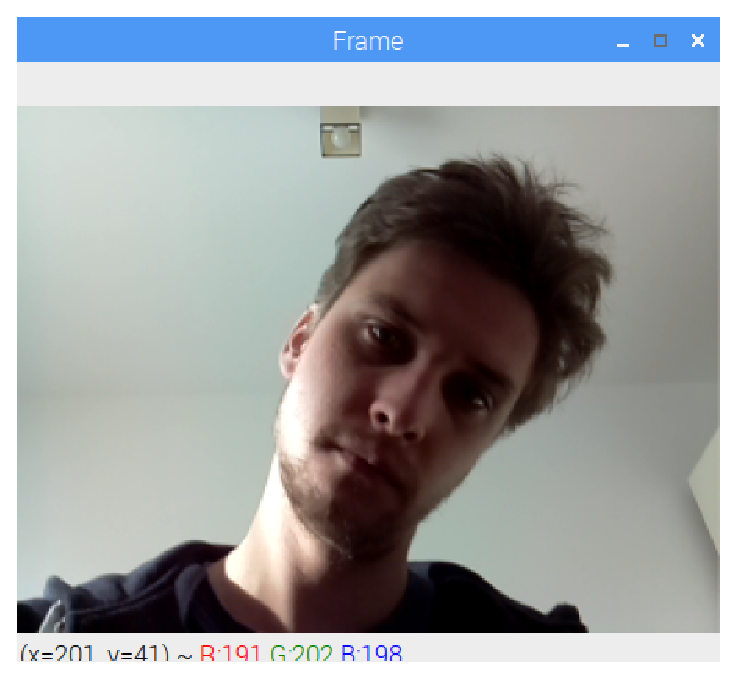
\includegraphics[width=.8\linewidth]{eps/mp_left_tilted_view.eps}
		\caption{Volto inclinato a sinistra.}
	\end{subfigure}
	\hspace{5mm}
	\begin{subfigure}{.3\textwidth}
		\centering
		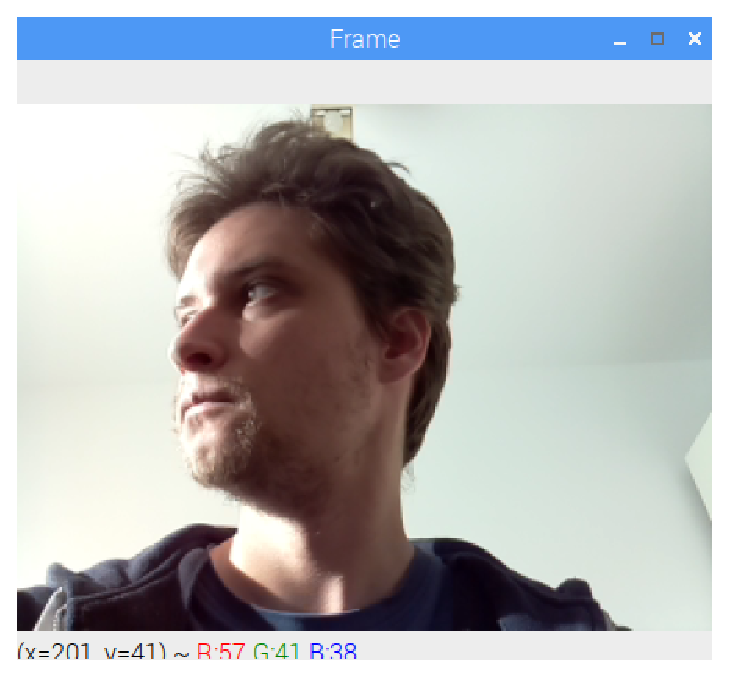
\includegraphics[width=.8\linewidth]{eps/mp_full_right_view.eps}
		\caption{Volto totalmente rivolto a destra.}
	\end{subfigure}
	\hspace{5mm}
	\begin{subfigure}{.3\textwidth}
		\centering
		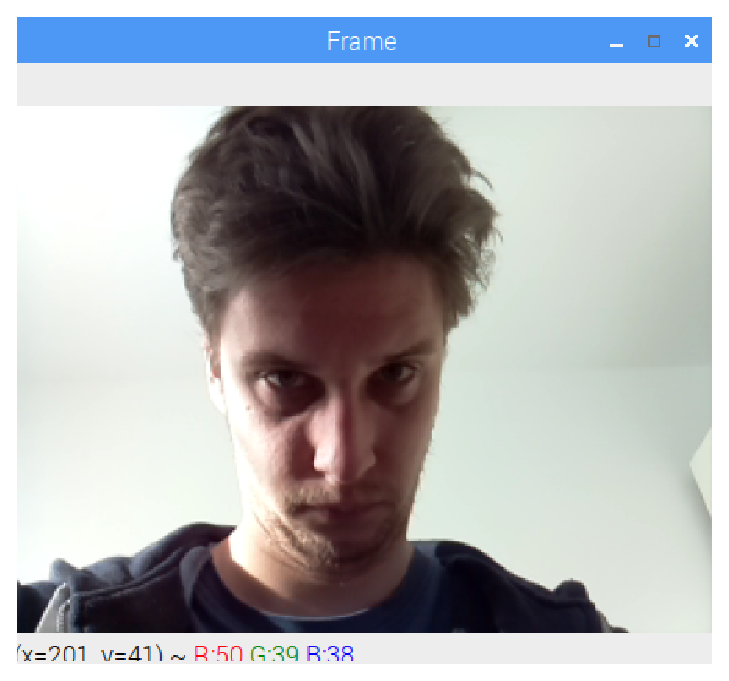
\includegraphics[width=.8\linewidth]{eps/mp_downward_view.eps}
		\caption{Volto rivolto verso il basso.}
	\end{subfigure}
	\caption{Localizzazione del volto con diverse angolazioni facciali.}
	\label{fig:face_poses}
\end{figure}

% pose testa (However, the Dlib Framework is not able to detect different positions of the driver's face such as turning the head completely right or left. In this case, these images are removed from the used dataset.)

\subsection{Costruzione dataset}
% ragioni per farsene uno proprio (non reperibilità, camera ecc.)
\subsubsection{Definizione delle categorie}
\subsubsection{Acquisizione video}
% Presentazione dello script dei 30 secondi
% Posizionamento camera e distanza in macchina
% Foto esempio
\subsubsection{Nomenclatura}

\subsection{Prestazioni}

\begin{equation}
Accuracy = \frac{TP + TN}{TP + TN + FP + FN} \times 100
\end{equation}

\begin{equation}
Precision = \frac{TP}{TP + FP} \times 100
\end{equation}

\begin{equation}
MisclassificationRate = \frac{FP + FN}{TP + TN + FP + FN} \times 100
\end{equation}

\begin{equation}
TPR = \frac{TP}{TP + FN} \times 100
\end{equation}

\begin{equation}
FPR = \frac{FP}{TN + FP} \times 100
\end{equation}

\begin{table}[h]
	\centering
	\begin{tabular}{cc|c|c|}
		\cline{3-4}
		&        & \multicolumn{2}{c|}{Predicted} \\ \cline{3-4} 
		&        & Alert         & Drowsy         \\ \hline
		\multicolumn{1}{|c|}{\multirow{2}{*}{Given}} & Alert  & TN & FP\\ \cline{2-4} 
		\multicolumn{1}{|c|}{}                       & Drowsy & FN & TP\\ \hline
	\end{tabular}
	\caption{Matrice di confusione con $EAR_{th}=0.3$.}
	\label{table:cm_0_3}
\end{table}

% For most of the subjects who wore glasses, negligible accuracy values were observed. This can be attributed to the fact that the Dlib shape predictor library often mistakes the upper boundaries of the lenses as the upper eyelids. This phenomenon was observed multiple times during testing. For example, in the case of one subject, we could easily perceive the upper contour settling over the upper boundary of the lens just a few frames into the video stream.

\begin{center}
	\framebox{\begin{tikzpicture}
		\begin{axis}[
		title={\textbf{ROC Curve}},
		width=0.8\textwidth,
		height=0.6\textwidth,
		axis x line=bottom,
		xlabel near ticks,
		xticklabel style={/pgf/number format/1000 sep=},
		axis y line=left,
		xmin=0,
		xmax=20,
		xlabel=Rate of False Positive (\%),
		ymin=0,
		ymax=50,
		ylabel=Rate of True Positive (\%)
		]
		\addplot[color=blue,mark=x] coordinates {
			(19.02, 43.66)
			(8.84, 30.71)
			(3.56, 22.33)
			(0.97, 12.97)
			(0.26, 8.29) };
		\legend{DrowsinessDetector\\}
		\end{axis}
	\end{tikzpicture}}
\end{center}


\begin{figure}[!htb]
	\centering
	\begin{tikzpicture}
		\begin{axis}[
			width  = 0.85*\textwidth,
			height = 13cm,
			major x tick style = transparent,
			ybar=3*\pgflinewidth,
			bar width=14pt,
			ymajorgrids = true,
			ylabel = {Run time speed},
			symbolic x coords={MP, GF},
			yticklabel style={
				/pgf/number format/fixed,
				/pgf/number format/precision=2
			},
			ytick = {0.02,0.04,0.06,0.08,0.10,0.12,0.14,0.16,0.18,0.20,0.22,0.24,0.26,0.28,0.30,0.32,0.34,0.36,0.38,0.40},
			xtick = data,
			scaled y ticks = false,
			enlarge x limits=0.5,
			ymin=0,
			legend style={
				at={(0.5,-0.1)},
				anchor=north,
				draw=none,
				fill=none,
				legend columns=1,
				column sep=5pt
			},
		]
		
		%Max EAR Open
		\addplot[style={bblue1,fill=bblue1,mark=none}]
		coordinates {(MP,0.36) (GF,0.30)};	
		
		%Max EAR Closed
		\addplot[style={ppurple2,fill=ppurple2,mark=none}]
		coordinates {(MP,0.26) (GF,0.20)};
		
		%Min EAR Open MP
		\node[
		draw=none,
		anchor=south east,
		fill=bblue2,
		minimum width=14pt,
		minimum height=230pt,
		xshift=-0.5pt]{};
		
		%Min EAR Open GF
		\node[
		draw=none,
		anchor=south east,
		fill=bblue2,
		minimum width=14pt,
		minimum height=180pt,
		xshift=155pt]{};	
		
		\legend{EAR range with open eyes, Max EAR with closed eyes}
		\end{axis}
	\end{tikzpicture}
\end{figure}

\iffalse
Esporre lo stato di funzionamento effettivo del sistema progettato ad elaborato concluso. Per ciascuna delle funzionalità salienti devono essere tabellate e discusse le performance riscontrate mediante opportuni test eseguiti in fase di validazione del progetto.\\

I tempi di esecuzione/comunicazione devono essere accompagnati dalle caratteristiche dell'hardware sul quale è eseguito il software.\\

Qualora l'elaborato includa algoritmi innovativi, indicarne la complessità computazionale (avendo cura di esporre lo pseudo codice nella sezione \ref{sec:implementazione}).\\


Vincoli circa la lunghezza della sezione (escluse didascalie, tabelle, testo nelle immagini, schemi):

\vspace{1cm}
\begin{tabular}{l|rr}
 & Numero minimo di battute & Numero massimo di battute \\
 \hline
 1 componente & 2000 & 3000 \\
 2 componenti & 2500 & 4500 \\
 3 componenti & 3000 & 6000 \\
 \hline
\end{tabular}
\fi

\newpage


%----------------------------------------------------------------------------------------
%	ANALISI DI DEPLOYMENT SU LARGA SCALA
%----------------------------------------------------------------------------------------

\section{Analisi di deployment su larga scala}

In questa sezione va discussa, eventualmente con l'ausilio di opportuni diagrammi (componenti, deployment), l'evoluzione del progetto presentato immaginando che venga adottato su larga scala. I dettagli qui esposti devono quindi astrarre dalle specifiche dell'elaborato qualora l'implementazione sia stata focalizzata su uno scenario isolato.\\

A titolo d’esempio, qualora applicabile, devono essere evidenziate le criticità che si potrebbero incontrare e devono essere proposte soluzioni tipiche in contesti di \textit{cloud architecture} per garantire un'adeguata \textit{resilienza}, in termini di \textit{availability} e \textit{scalability} del sistema.\\


Vincoli circa la lunghezza della sezione (escluse didascalie, tabelle, testo nelle immagini, schemi):

\vspace{1cm}
\begin{tabular}{l|rr}
 & Numero minimo di battute & Numero massimo di battute \\
 \hline
 1 componente & 3000 & 6000 \\
 2 componenti & 4500 & 9000 \\
 3 componenti & 6000 & 12000 \\
 \hline
\end{tabular}


\newpage


%----------------------------------------------------------------------------------------
%	PIANO DI LAVORO
%----------------------------------------------------------------------------------------

\section{Piano di lavoro}

In questa sezione devono essere chiariti i compiti svolti da ciascun candidato nel caso in cui il gruppo abbia più di un componente.\\

Deve essere inoltre esposto il piano di lavoro adottato. A tal fine, per ogni attività svolta durante la preparazione dell'elaborato (ad esempio: studio di una tecnologia, progettazione di un componente, implementazione di un algoritmo ecc…) deve essere chiarita la collocazione temporale e devono essere indicate le risorse impiegate per svolgerla (giorni/uomo). I candidati possono ricorrere a opportuni diagrammi come quello di Gantt.\\


Vincoli circa la lunghezza della sezione (escluse didascalie, tabelle, testo nelle immagini, schemi):

\vspace{1cm}
\begin{tabular}{l|rr}
 & Numero minimo di battute & Numero massimo di battute \\
 \hline
 1 componente & 1000 & 2000 \\
 2 componenti & 1500 & 3000 \\
 3 componenti & 2000 & 4000 \\
 \hline
\end{tabular}

\newpage


%----------------------------------------------------------------------------------------
%	CONCLUSIONI
%----------------------------------------------------------------------------------------

\section{Conclusioni}

Calibrazione soglia EAR per utente.

If a face is detected, then a region of interest in marked within the face. This region of interest contains the eyes. Defining a region of interest significantly reduces the computational requirements of the system. After that the eyes are detected from the region of interest.

However, it has been found that the rate of detecting the correct feature, or the percentage of success among a number of detection attempts, varies depending on the application and number of classes. The determination of drowsiness using PERCLOS and Eye Blink has a success rate of close to 100\% [43] and 98\% [45], respectively. However it has to be noted that, the high positive detection rate achieved by [43] was when the subjects didn’t wear glasses. Likewise, as most researchers conducted their experiments in simulated environment they achieved a higher success rate. The positive detection rate decreased significantly when the experiment was carried out in a real environment [15].
Another limitation of behavioral measure was brought out in an experiment conducted by Golz et al. They evaluated various drowsiness monitoring commercial products, and observed that driver state cannot be correlated to driving performance and vehicle status based on behavioral measures alone [57].

Passaggio a HW più potente.

Esporre brevemente le considerazioni conclusive sul progetto presentato, indicando anche i possibili sviluppi futuri.\\

Vincoli circa la lunghezza della sezione (escluse didascalie, tabelle, testo nelle immagini, schemi):

\vspace{1cm}
\begin{tabular}{l|rr}
 & Numero minimo di battute & Numero massimo di battute \\
 \hline
 1 componente & 500 & 1000 \\
 2 componenti & 1000 & 2000 \\
 3 componenti & 1500 & 3000 \\
 \hline
\end{tabular}

\newpage


%----------------------------------------------------------------------------------------
%	APPENDICE
%----------------------------------------------------------------------------------------

\appendix
\addcontentsline{toc}{section}{Appendice}
\section*{Appendice}


% EAR = 0.30
\begin{landscape}
	\begin{table}[]
		\centering
		\begin{adjustbox}{width=1.4\textwidth}
			\begin{tabular}{lllllllllllllllccllll}
				& & & & & & & & & & & & & & & \multicolumn{1}{l}{} & \multicolumn{1}{l}{} & & & &\\ \cline{5-21}
				& & & \multicolumn{1}{l|}{} & \multicolumn{4}{c|}{Confusion Matrix} & \multicolumn{7}{c|}{Category Statistical Indices} & \multicolumn{3}{c|}{Daytime Statistical Indices} & \multicolumn{3}{c|}{Global Statistical Indices}\\ \hline
				\multicolumn{4}{|c|}{Category} & \multicolumn{1}{c|}{TP} & \multicolumn{1}{c|}{TN} & \multicolumn{1}{c|}{FP} & \multicolumn{1}{c|}{FN} & \multicolumn{1}{c|}{ACC} & \multicolumn{1}{c|}{PRE} & \multicolumn{1}{c|}{MR} & \multicolumn{1}{c|}{TPR} & \multicolumn{1}{c|}{TNR} & \multicolumn{1}{c|}{FPR} & \multicolumn{1}{c|}{FNR} & \multicolumn{1}{c|}{ACC} & \multicolumn{1}{c|}{TPR} & \multicolumn{1}{c|}{FPR} & \multicolumn{1}{c|}{ACC} & \multicolumn{1}{c|}{TPR} & \multicolumn{1}{c|}{FPR}\\ \hline
				\multicolumn{1}{|l|}{\multirow{8}{*}{Day}} & \multicolumn{1}{l|}{\multirow{4}{*}{Drowsiness}} & \multicolumn{1}{l|}{\multirow{2}{*}{Glasses}} & \multicolumn{1}{l|}{Static} & \multicolumn{1}{l|}{372} & \multicolumn{1}{l|}{2005} & \multicolumn{1}{l|}{501} & \multicolumn{1}{l|}{702} & \multicolumn{1}{l|}{66,40} & \multicolumn{1}{l|}{42,61} & \multicolumn{1}{l|}{33,60} & \multicolumn{1}{l|}{34,64} & \multicolumn{1}{l|}{80,01} & \multicolumn{1}{l|}{19,99} & \multicolumn{1}{l|}{65,36} & \multicolumn{1}{c|}{\multirow{8}{*}{87,57}} & \multicolumn{1}{c|}{\multirow{8}{*}{53,35}} & \multicolumn{1}{c|}{\multirow{8}{*}{6,85}} & \multicolumn{1}{c|}{\multirow{16}{*}{74,64}} & \multicolumn{1}{c|}{\multirow{16}{*}{43,66}} & \multicolumn{1}{c|}{\multirow{16}{*}{19,02}}\\ \cline{4-15}
				\multicolumn{1}{|l|}{} & \multicolumn{1}{l|}{} & \multicolumn{1}{l|}{} & \multicolumn{1}{l|}{Dynamic} & \multicolumn{1}{l|}{163} & \multicolumn{1}{l|}{1870} & \multicolumn{1}{l|}{78} & \multicolumn{1}{l|}{574} & \multicolumn{1}{l|}{75,72} & \multicolumn{1}{l|}{67,63} & \multicolumn{1}{l|}{24,28} & \multicolumn{1}{l|}{22,12} & \multicolumn{1}{l|}{95,96} & \multicolumn{1}{l|}{4,00} & \multicolumn{1}{l|}{77,88} & \multicolumn{1}{c|}{} & \multicolumn{1}{c|}{} & \multicolumn{1}{l|}{} & \multicolumn{1}{l|}{} & \multicolumn{1}{l|}{} & \multicolumn{1}{l|}{}\\ \cline{3-15}
				\multicolumn{1}{|l|}{} & \multicolumn{1}{l|}{} & \multicolumn{1}{l|}{\multirow{2}{*}{NoGlasses}} & \multicolumn{1}{l|}{Static}  & \multicolumn{1}{l|}{1409} & \multicolumn{1}{l|}{3141} & \multicolumn{1}{l|}{357} & \multicolumn{1}{l|}{463} & \multicolumn{1}{l|}{84,73} & \multicolumn{1}{l|}{79,78} & \multicolumn{1}{l|}{15,27} & \multicolumn{1}{l|}{75,27} & \multicolumn{1}{l|}{89,79} & \multicolumn{1}{l|}{10,21} & \multicolumn{1}{l|}{24,73} & \multicolumn{1}{c|}{} & \multicolumn{1}{c|}{} & \multicolumn{1}{l|}{} & \multicolumn{1}{l|}{} & \multicolumn{1}{l|}{} & \multicolumn{1}{l|}{}\\ \cline{4-15}
				\multicolumn{1}{|l|}{} & \multicolumn{1}{l|}{} & \multicolumn{1}{l|}{} & \multicolumn{1}{l|}{Dynamic} & \multicolumn{1}{l|}{991} & \multicolumn{1}{l|}{2319} & \multicolumn{1}{l|}{43} & \multicolumn{1}{l|}{227} & \multicolumn{1}{l|}{92,46} & \multicolumn{1}{l|}{95,84} & \multicolumn{1}{l|}{7,54} & \multicolumn{1}{l|}{81,36} & \multicolumn{1}{l|}{98,18} & \multicolumn{1}{l|}{1,82} & \multicolumn{1}{l|}{18,64} & \multicolumn{1}{c|}{} & \multicolumn{1}{c|}{} & \multicolumn{1}{l|}{} & \multicolumn{1}{l|}{} & \multicolumn{1}{l|}{} & \multicolumn{1}{l|}{} \\ \cline{2-15}
				\multicolumn{1}{|l|}{} & \multicolumn{1}{l|}{\multirow{4}{*}{NoDrowsiness}} & \multicolumn{1}{l|}{\multirow{2}{*}{Glasses}} & \multicolumn{1}{l|}{Static} & \multicolumn{1}{l|}{0} & \multicolumn{1}{l|}{2390} & \multicolumn{1}{l|}{295} & \multicolumn{1}{l|}{0} & \multicolumn{1}{l|}{89,01} & \multicolumn{1}{l|}{N/A} & \multicolumn{1}{l|}{10,99} & \multicolumn{1}{l|}{N/A} & \multicolumn{1}{l|}{89,01} & \multicolumn{1}{l|}{10,99} & \multicolumn{1}{l|}{N/A} & \multicolumn{1}{c|}{} & \multicolumn{1}{c|}{} & \multicolumn{1}{l|}{} & \multicolumn{1}{l|}{} & \multicolumn{1}{l|}{} & \multicolumn{1}{l|}{}\\ \cline{4-15}
				\multicolumn{1}{|l|}{} & \multicolumn{1}{l|}{} & \multicolumn{1}{l|}{} & \multicolumn{1}{l|}{Dynamic} & \multicolumn{1}{l|}{0} & \multicolumn{1}{l|}{1749} & \multicolumn{1}{l|}{41} & \multicolumn{1}{l|}{0} & \multicolumn{1}{l|}{97,71} & \multicolumn{1}{l|}{N/A} & \multicolumn{1}{l|}{2,30} & \multicolumn{1}{l|}{N/A} & \multicolumn{1}{l|}{97,71} & \multicolumn{1}{l|}{2,30} & \multicolumn{1}{l|}{N/A} & \multicolumn{1}{c|}{} & \multicolumn{1}{c|}{} & \multicolumn{1}{l|}{} & \multicolumn{1}{l|}{} & \multicolumn{1}{l|}{} & \multicolumn{1}{l|}{}\\ \cline{3-15}
				\multicolumn{1}{|l|}{} & \multicolumn{1}{l|}{} & \multicolumn{1}{l|}{\multirow{2}{*}{NoGlasses}} & \multicolumn{1}{l|}{Static} & \multicolumn{1}{l|}{0} & \multicolumn{1}{l|}{2633} & \multicolumn{1}{l|}{52} & \multicolumn{1}{l|}{0} & \multicolumn{1}{l|}{98,06} & \multicolumn{1}{l|}{N/A} & \multicolumn{1}{l|}{1,94} & \multicolumn{1}{l|}{N/A} & \multicolumn{1}{l|}{98,06} & \multicolumn{1}{l|}{1,94} & \multicolumn{1}{l|}{N/A} & \multicolumn{1}{c|}{} & \multicolumn{1}{c|}{} & \multicolumn{1}{l|}{} & \multicolumn{1}{l|}{} & \multicolumn{1}{l|}{} & \multicolumn{1}{l|}{} \\ \cline{4-15}
				\multicolumn{1}{|l|}{} & \multicolumn{1}{l|}{} & \multicolumn{1}{l|}{} & \multicolumn{1}{l|}{Dynamic} & \multicolumn{1}{l|}{0} & \multicolumn{1}{l|}{2590} & \multicolumn{1}{l|}{95} & \multicolumn{1}{l|}{0} & \multicolumn{1}{l|}{96,46} & \multicolumn{1}{l|}{N/A} & \multicolumn{1}{l|}{3,54} & \multicolumn{1}{l|}{N/A} & \multicolumn{1}{l|}{96,46} & \multicolumn{1}{l|}{3,54} & \multicolumn{1}{l|}{N/A} & \multicolumn{1}{c|}{} & \multicolumn{1}{c|}{} & \multicolumn{1}{l|}{} & \multicolumn{1}{l|}{} & \multicolumn{1}{l|}{} & \multicolumn{1}{l|}{}\\ \cline{1-18}
				\multicolumn{1}{|l|}{\multirow{8}{*}{Night}} & \multicolumn{1}{l|}{\multirow{4}{*}{Drowsiness}} & \multicolumn{1}{l|}{\multirow{2}{*}{Glasses}} & \multicolumn{1}{l|}{Static} & \multicolumn{1}{l|}{327} & \multicolumn{1}{l|}{1015} & \multicolumn{1}{l|}{186} & \multicolumn{1}{l|}{262} & \multicolumn{1}{l|}{74,97} & \multicolumn{1}{l|}{63,74} & \multicolumn{1}{l|}{25,03} & \multicolumn{1}{l|}{55,52} & \multicolumn{1}{l|}{84,51} & \multicolumn{1}{l|}{15,49} & \multicolumn{1}{l|}{44,48} & \multicolumn{1}{c|}{\multirow{8}{*}{61,70}} & \multicolumn{1}{c|}{\multirow{8}{*}{33,96}} & \multicolumn{1}{c|}{\multirow{8}{*}{31,18}} & \multicolumn{1}{l|}{} & \multicolumn{1}{l|}{} & \multicolumn{1}{l|}{} \\ \cline{4-15}
				\multicolumn{1}{|l|}{} & \multicolumn{1}{l|}{} & \multicolumn{1}{l|}{} & \multicolumn{1}{l|}{Dynamic} & \multicolumn{1}{l|}{103} & \multicolumn{1}{l|}{392} & \multicolumn{1}{l|}{978} & \multicolumn{1}{l|}{317} & \multicolumn{1}{l|}{27,65} & \multicolumn{1}{l|}{9,53} & \multicolumn{1}{l|}{72,35} & \multicolumn{1}{l|}{24,52} & \multicolumn{1}{l|}{28,61} & \multicolumn{1}{l|}{71,39} & \multicolumn{1}{l|}{75,48} & \multicolumn{1}{c|}{} & \multicolumn{1}{c|}{} & \multicolumn{1}{l|}{} & \multicolumn{1}{l|}{} & \multicolumn{1}{l|}{} & \multicolumn{1}{l|}{}\\ \cline{3-15}
				\multicolumn{1}{|l|}{} & \multicolumn{1}{l|}{} & \multicolumn{1}{l|}{\multirow{2}{*}{NoGlasses}} & \multicolumn{1}{l|}{Static} & \multicolumn{1}{l|}{259} & \multicolumn{1}{l|}{1376} & \multicolumn{1}{l|}{160} & \multicolumn{1}{l|}{890} & \multicolumn{1}{l|}{60,89} & \multicolumn{1}{l|}{61,81} & \multicolumn{1}{l|}{39,11} & \multicolumn{1}{l|}{22,54} & \multicolumn{1}{l|}{89,58} & \multicolumn{1}{l|}{10,42} & \multicolumn{1}{l|}{77,46} & \multicolumn{1}{c|}{} & \multicolumn{1}{c|}{} & \multicolumn{1}{l|}{} & \multicolumn{1}{l|}{} & \multicolumn{1}{l|}{} & \multicolumn{1}{l|}{} \\ \cline{4-15}
				\multicolumn{1}{|l|}{} & \multicolumn{1}{l|}{} & \multicolumn{1}{l|}{} & \multicolumn{1}{l|}{Dynamic} & \multicolumn{1}{l|}{314} & \multicolumn{1}{l|}{1447} & \multicolumn{1}{l|}{294} & \multicolumn{1}{l|}{630} & \multicolumn{1}{l|}{65,59} & \multicolumn{1}{l|}{51,64} & \multicolumn{1}{l|}{34,41} & \multicolumn{1}{l|}{33,26} & \multicolumn{1}{l|}{83,11} & \multicolumn{1}{l|}{16,89} & \multicolumn{1}{l|}{66,74} & \multicolumn{1}{c|}{} & \multicolumn{1}{c|}{} & \multicolumn{1}{l|}{} & \multicolumn{1}{l|}{} & \multicolumn{1}{l|}{} & \multicolumn{1}{l|}{} \\ \cline{2-15}
				\multicolumn{1}{|l|}{} & \multicolumn{1}{l|}{\multirow{4}{*}{NoDrowsiness}} & \multicolumn{1}{l|}{\multirow{2}{*}{Glasses}} & \multicolumn{1}{l|}{Static} & \multicolumn{1}{l|}{0} & \multicolumn{1}{l|}{1330} & \multicolumn{1}{l|}{460} & \multicolumn{1}{l|}{0} & \multicolumn{1}{l|}{74,30} & \multicolumn{1}{l|}{N/A} & \multicolumn{1}{l|}{25,70} & \multicolumn{1}{l|}{N/A} & \multicolumn{1}{l|}{74,30} & \multicolumn{1}{l|}{25,70} & \multicolumn{1}{l|}{N/A} & \multicolumn{1}{c|}{} & \multicolumn{1}{c|}{} & \multicolumn{1}{l|}{} & \multicolumn{1}{l|}{} & \multicolumn{1}{l|}{} & \multicolumn{1}{l|}{} \\ \cline{4-15}
				\multicolumn{1}{|l|}{} & \multicolumn{1}{l|}{} & \multicolumn{1}{l|}{} & \multicolumn{1}{l|}{Dynamic} & \multicolumn{1}{l|}{0} & \multicolumn{1}{l|}{655} & \multicolumn{1}{l|}{1135} & \multicolumn{1}{l|}{0} & \multicolumn{1}{l|}{36,59} & \multicolumn{1}{l|}{N/A} & \multicolumn{1}{l|}{63,41} & \multicolumn{1}{l|}{N/A} & \multicolumn{1}{l|}{36,59} & \multicolumn{1}{l|}{63,41} & \multicolumn{1}{l|}{N/A} & \multicolumn{1}{c|}{} & \multicolumn{1}{c|}{} & \multicolumn{1}{l|}{} & \multicolumn{1}{l|}{} & \multicolumn{1}{l|}{} & \multicolumn{1}{l|}{} \\ \cline{3-15}
				\multicolumn{1}{|l|}{} & \multicolumn{1}{l|}{} & \multicolumn{1}{l|}{\multirow{2}{*}{NoGlasses}} & \multicolumn{1}{l|}{Static}  & \multicolumn{1}{l|}{0} & \multicolumn{1}{l|}{1542} & \multicolumn{1}{l|}{248} & \multicolumn{1}{l|}{0} & \multicolumn{1}{l|}{86,15} & \multicolumn{1}{l|}{N/A} & \multicolumn{1}{l|}{13,85} & \multicolumn{1}{l|}{N/A} & \multicolumn{1}{l|}{86,15} & \multicolumn{1}{l|}{13,85} & \multicolumn{1}{l|}{N/A} & \multicolumn{1}{c|}{} & \multicolumn{1}{c|}{} & \multicolumn{1}{l|}{} & \multicolumn{1}{l|}{} & \multicolumn{1}{l|}{} & \multicolumn{1}{l|}{} \\ \cline{4-15}
				\multicolumn{1}{|l|}{} & \multicolumn{1}{l|}{} & \multicolumn{1}{l|}{} & \multicolumn{1}{l|}{Dynamic} & \multicolumn{1}{l|}{0} & \multicolumn{1}{l|}{1207} & \multicolumn{1}{l|}{583} & \multicolumn{1}{l|}{0} & \multicolumn{1}{l|}{67,43} & \multicolumn{1}{l|}{N/A} & \multicolumn{1}{l|}{32,57} & \multicolumn{1}{l|}{N/A} & \multicolumn{1}{l|}{67,43} & \multicolumn{1}{l|}{32,57} & \multicolumn{1}{l|}{N/A} & \multicolumn{1}{c|}{} & \multicolumn{1}{c|}{} & \multicolumn{1}{l|}{} & \multicolumn{1}{l|}{} & \multicolumn{1}{l|}{} & \multicolumn{1}{l|}{} \\ \hline
				& & & & & & & & & & & & & & & \multicolumn{1}{l}{} & \multicolumn{1}{l}{} & & & &
			\end{tabular}
		\end{adjustbox}
		\caption{Accuratezza del rilevatore di sonnolenza con $EAR_{th}=0.3$.}
		\label{table:global_ear_30}
	\end{table}
\end{landscape}

% EAR = 0.28
\begin{landscape}
	\begin{table}[]
		\centering
		\begin{adjustbox}{width=1.4\textwidth}
			\begin{tabular}{lllllllllllllllccllll}
				& & & & & & & & & & & & & & & \multicolumn{1}{l}{} & \multicolumn{1}{l}{} & & & &\\ \cline{5-21}
				& & & \multicolumn{1}{l|}{} & \multicolumn{4}{c|}{Confusion Matrix} & \multicolumn{7}{c|}{Category Statistical Indices} & \multicolumn{3}{c|}{Daytime Statistical Indices} & \multicolumn{3}{c|}{Global Statistical Indices}\\ \hline
				\multicolumn{4}{|c|}{Category} & \multicolumn{1}{c|}{TP} & \multicolumn{1}{c|}{TN} & \multicolumn{1}{c|}{FP} & \multicolumn{1}{c|}{FN} & \multicolumn{1}{c|}{ACC} & \multicolumn{1}{c|}{PRE} & \multicolumn{1}{c|}{MR} & \multicolumn{1}{c|}{TPR} & \multicolumn{1}{c|}{TNR} & \multicolumn{1}{c|}{FPR} & \multicolumn{1}{c|}{FNR} & \multicolumn{1}{c|}{ACC} & \multicolumn{1}{c|}{TPR} & \multicolumn{1}{c|}{FPR} & \multicolumn{1}{c|}{ACC} & \multicolumn{1}{c|}{TPR} & \multicolumn{1}{c|}{FPR}\\ \hline
				\multicolumn{1}{|l|}{\multirow{8}{*}{Day}} & \multicolumn{1}{l|}{\multirow{4}{*}{Drowsiness}} & \multicolumn{1}{l|}{\multirow{2}{*}{Glasses}} & \multicolumn{1}{l|}{Static} & \multicolumn{1}{l|}{332} & \multicolumn{1}{l|}{2287} & \multicolumn{1}{l|}{219} & \multicolumn{1}{l|}{742} & \multicolumn{1}{l|}{73,16} & \multicolumn{1}{l|}{60,25} & \multicolumn{1}{l|}{26,84} & \multicolumn{1}{l|}{30,91} & \multicolumn{1}{l|}{91,26} & \multicolumn{1}{l|}{8,74} & \multicolumn{1}{l|}{69,09} & \multicolumn{1}{c|}{\multirow{8}{*}{89,73}} & \multicolumn{1}{c|}{\multirow{8}{*}{46,62}} & \multicolumn{1}{c|}{\multirow{8}{*}{2,73}} & \multicolumn{1}{c|}{\multirow{16}{*}{81,19}} & \multicolumn{1}{c|}{\multirow{16}{*}{30,71}} & \multicolumn{1}{c|}{\multirow{16}{*}{8,84}}\\ \cline{4-15}
				\multicolumn{1}{|l|}{} & \multicolumn{1}{l|}{} & \multicolumn{1}{l|}{} & \multicolumn{1}{l|}{Dynamic} & \multicolumn{1}{l|}{144} & \multicolumn{1}{l|}{1898} & \multicolumn{1}{l|}{50} & \multicolumn{1}{l|}{593} & \multicolumn{1}{l|}{76,05} & \multicolumn{1}{l|}{74,23} & \multicolumn{1}{l|}{23,95} & \multicolumn{1}{l|}{19,54} & \multicolumn{1}{l|}{97,43} & \multicolumn{1}{l|}{3,57} & \multicolumn{1}{l|}{80,46} & \multicolumn{1}{c|}{} & \multicolumn{1}{c|}{} & \multicolumn{1}{l|}{} & \multicolumn{1}{l|}{} & \multicolumn{1}{l|}{} & \multicolumn{1}{l|}{}\\ \cline{3-15}
				\multicolumn{1}{|l|}{} & \multicolumn{1}{l|}{} & \multicolumn{1}{l|}{\multirow{2}{*}{NoGlasses}} & \multicolumn{1}{l|}{Static}  & \multicolumn{1}{l|}{1194} & \multicolumn{1}{l|}{3411} & \multicolumn{1}{l|}{87} & \multicolumn{1}{l|}{678} & \multicolumn{1}{l|}{85,75} & \multicolumn{1}{l|}{93,21} & \multicolumn{1}{l|}{14,25} & \multicolumn{1}{l|}{63,78} & \multicolumn{1}{l|}{97,51} & \multicolumn{1}{l|}{2,49} & \multicolumn{1}{l|}{36,22} & \multicolumn{1}{c|}{} & \multicolumn{1}{c|}{} & \multicolumn{1}{l|}{} & \multicolumn{1}{l|}{} & \multicolumn{1}{l|}{} & \multicolumn{1}{l|}{}\\ \cline{4-15}
				\multicolumn{1}{|l|}{} & \multicolumn{1}{l|}{} & \multicolumn{1}{l|}{} & \multicolumn{1}{l|}{Dynamic} & \multicolumn{1}{l|}{880} & \multicolumn{1}{l|}{2339} & \multicolumn{1}{l|}{23} & \multicolumn{1}{l|}{338} & \multicolumn{1}{l|}{89,92} & \multicolumn{1}{l|}{97,45} & \multicolumn{1}{l|}{10,08} & \multicolumn{1}{l|}{72,25} & \multicolumn{1}{l|}{99,03} & \multicolumn{1}{l|}{0,97} & \multicolumn{1}{l|}{27,75} & \multicolumn{1}{c|}{} & \multicolumn{1}{c|}{} & \multicolumn{1}{l|}{} & \multicolumn{1}{l|}{} & \multicolumn{1}{l|}{} & \multicolumn{1}{l|}{} \\ \cline{2-15}
				\multicolumn{1}{|l|}{} & \multicolumn{1}{l|}{\multirow{4}{*}{NoDrowsiness}} & \multicolumn{1}{l|}{\multirow{2}{*}{Glasses}} & \multicolumn{1}{l|}{Static} & \multicolumn{1}{l|}{0} & \multicolumn{1}{l|}{2540} & \multicolumn{1}{l|}{145} & \multicolumn{1}{l|}{0} & \multicolumn{1}{l|}{94,60} & \multicolumn{1}{l|}{N/A} & \multicolumn{1}{l|}{5,40} & \multicolumn{1}{l|}{N/A} & \multicolumn{1}{l|}{94,60} & \multicolumn{1}{l|}{5,40} & \multicolumn{1}{l|}{N/A} & \multicolumn{1}{c|}{} & \multicolumn{1}{c|}{} & \multicolumn{1}{l|}{} & \multicolumn{1}{l|}{} & \multicolumn{1}{l|}{} & \multicolumn{1}{l|}{}\\ \cline{4-15}
				\multicolumn{1}{|l|}{} & \multicolumn{1}{l|}{} & \multicolumn{1}{l|}{} & \multicolumn{1}{l|}{Dynamic} & \multicolumn{1}{l|}{0} & \multicolumn{1}{l|}{1782} & \multicolumn{1}{l|}{8} & \multicolumn{1}{l|}{0} & \multicolumn{1}{l|}{99,55} & \multicolumn{1}{l|}{N/A} & \multicolumn{1}{l|}{0,45} & \multicolumn{1}{l|}{N/A} & \multicolumn{1}{l|}{99,55} & \multicolumn{1}{l|}{0,45} & \multicolumn{1}{l|}{N/A} & \multicolumn{1}{c|}{} & \multicolumn{1}{c|}{} & \multicolumn{1}{l|}{} & \multicolumn{1}{l|}{} & \multicolumn{1}{l|}{} & \multicolumn{1}{l|}{}\\ \cline{3-15}
				\multicolumn{1}{|l|}{} & \multicolumn{1}{l|}{} & \multicolumn{1}{l|}{\multirow{2}{*}{NoGlasses}} & \multicolumn{1}{l|}{Static} & \multicolumn{1}{l|}{0} & \multicolumn{1}{l|}{2659} & \multicolumn{1}{l|}{26} & \multicolumn{1}{l|}{0} & \multicolumn{1}{l|}{99,03} & \multicolumn{1}{l|}{N/A} & \multicolumn{1}{l|}{0,97} & \multicolumn{1}{l|}{N/A} & \multicolumn{1}{l|}{99,03} & \multicolumn{1}{l|}{0,97} & \multicolumn{1}{l|}{N/A} & \multicolumn{1}{c|}{} & \multicolumn{1}{c|}{} & \multicolumn{1}{l|}{} & \multicolumn{1}{l|}{} & \multicolumn{1}{l|}{} & \multicolumn{1}{l|}{} \\ \cline{4-15}
				\multicolumn{1}{|l|}{} & \multicolumn{1}{l|}{} & \multicolumn{1}{l|}{} & \multicolumn{1}{l|}{Dynamic} & \multicolumn{1}{l|}{0} & \multicolumn{1}{l|}{2679} & \multicolumn{1}{l|}{6} & \multicolumn{1}{l|}{0} & \multicolumn{1}{l|}{99,78} & \multicolumn{1}{l|}{N/A} & \multicolumn{1}{l|}{0,22} & \multicolumn{1}{l|}{N/A} & \multicolumn{1}{l|}{99,78} & \multicolumn{1}{l|}{0,22} & \multicolumn{1}{l|}{N/A} & \multicolumn{1}{c|}{} & \multicolumn{1}{c|}{} & \multicolumn{1}{l|}{} & \multicolumn{1}{l|}{} & \multicolumn{1}{l|}{} & \multicolumn{1}{l|}{}\\ \cline{1-18}
				\multicolumn{1}{|l|}{\multirow{8}{*}{Night}} & \multicolumn{1}{l|}{\multirow{4}{*}{Drowsiness}} & \multicolumn{1}{l|}{\multirow{2}{*}{Glasses}} & \multicolumn{1}{l|}{Static} & \multicolumn{1}{l|}{145} & \multicolumn{1}{l|}{1142} & \multicolumn{1}{l|}{59} & \multicolumn{1}{l|}{444} & \multicolumn{1}{l|}{71,90} & \multicolumn{1}{l|}{71,08} & \multicolumn{1}{l|}{28,10} & \multicolumn{1}{l|}{24,62} & \multicolumn{1}{l|}{95,09} & \multicolumn{1}{l|}{4,91} & \multicolumn{1}{l|}{77,38} & \multicolumn{1}{c|}{\multirow{8}{*}{72,64}} & \multicolumn{1}{c|}{\multirow{8}{*}{14,81}} & \multicolumn{1}{c|}{\multirow{8}{*}{14,96}} & \multicolumn{1}{l|}{} & \multicolumn{1}{l|}{} & \multicolumn{1}{l|}{} \\ \cline{4-15}
				\multicolumn{1}{|l|}{} & \multicolumn{1}{l|}{} & \multicolumn{1}{l|}{} & \multicolumn{1}{l|}{Dynamic} & \multicolumn{1}{l|}{16} & \multicolumn{1}{l|}{963} & \multicolumn{1}{l|}{407} & \multicolumn{1}{l|}{404} & \multicolumn{1}{l|}{54,69} & \multicolumn{1}{l|}{3,78} & \multicolumn{1}{l|}{45,31} & \multicolumn{1}{l|}{3,81} & \multicolumn{1}{l|}{70,29} & \multicolumn{1}{l|}{29,71} & \multicolumn{1}{l|}{96,19} & \multicolumn{1}{c|}{} & \multicolumn{1}{c|}{} & \multicolumn{1}{l|}{} & \multicolumn{1}{l|}{} & \multicolumn{1}{l|}{} & \multicolumn{1}{l|}{}\\ \cline{3-15}
				\multicolumn{1}{|l|}{} & \multicolumn{1}{l|}{} & \multicolumn{1}{l|}{\multirow{2}{*}{NoGlasses}} & \multicolumn{1}{l|}{Static} & \multicolumn{1}{l|}{251} & \multicolumn{1}{l|}{1527} & \multicolumn{1}{l|}{9} & \multicolumn{1}{l|}{808} & \multicolumn{1}{l|}{68,52} & \multicolumn{1}{l|}{96,54} & \multicolumn{1}{l|}{31,48} & \multicolumn{1}{l|}{23,70} & \multicolumn{1}{l|}{99,41} & \multicolumn{1}{l|}{0,59} & \multicolumn{1}{l|}{76,30} & \multicolumn{1}{c|}{} & \multicolumn{1}{c|}{} & \multicolumn{1}{l|}{} & \multicolumn{1}{l|}{} & \multicolumn{1}{l|}{} & \multicolumn{1}{l|}{} \\ \cline{4-15}
				\multicolumn{1}{|l|}{} & \multicolumn{1}{l|}{} & \multicolumn{1}{l|}{} & \multicolumn{1}{l|}{Dynamic} & \multicolumn{1}{l|}{67} & \multicolumn{1}{l|}{1584} & \multicolumn{1}{l|}{157} & \multicolumn{1}{l|}{877} & \multicolumn{1}{l|}{61,49} & \multicolumn{1}{l|}{29,91} & \multicolumn{1}{l|}{38,51} & \multicolumn{1}{l|}{7,10} & \multicolumn{1}{l|}{90,98} & \multicolumn{1}{l|}{9,02} & \multicolumn{1}{l|}{92,90} & \multicolumn{1}{c|}{} & \multicolumn{1}{c|}{} & \multicolumn{1}{l|}{} & \multicolumn{1}{l|}{} & \multicolumn{1}{l|}{} & \multicolumn{1}{l|}{} \\ \cline{2-15}
				\multicolumn{1}{|l|}{} & \multicolumn{1}{l|}{\multirow{4}{*}{NoDrowsiness}} & \multicolumn{1}{l|}{\multirow{2}{*}{Glasses}} & \multicolumn{1}{l|}{Static} & \multicolumn{1}{l|}{0} & \multicolumn{1}{l|}{1648} & \multicolumn{1}{l|}{142} & \multicolumn{1}{l|}{0} & \multicolumn{1}{l|}{92,07} & \multicolumn{1}{l|}{N/A} & \multicolumn{1}{l|}{7,93} & \multicolumn{1}{l|}{N/A} & \multicolumn{1}{l|}{92,07} & \multicolumn{1}{l|}{7,93} & \multicolumn{1}{l|}{N/A} & \multicolumn{1}{c|}{} & \multicolumn{1}{c|}{} & \multicolumn{1}{l|}{} & \multicolumn{1}{l|}{} & \multicolumn{1}{l|}{} & \multicolumn{1}{l|}{} \\ \cline{4-15}
				\multicolumn{1}{|l|}{} & \multicolumn{1}{l|}{} & \multicolumn{1}{l|}{} & \multicolumn{1}{l|}{Dynamic} & \multicolumn{1}{l|}{0} & \multicolumn{1}{l|}{978} & \multicolumn{1}{l|}{812} & \multicolumn{1}{l|}{0} & \multicolumn{1}{l|}{54,64} & \multicolumn{1}{l|}{N/A} & \multicolumn{1}{l|}{45,36} & \multicolumn{1}{l|}{N/A} & \multicolumn{1}{l|}{54,64} & \multicolumn{1}{l|}{45,36} & \multicolumn{1}{l|}{N/A} & \multicolumn{1}{c|}{} & \multicolumn{1}{c|}{} & \multicolumn{1}{l|}{} & \multicolumn{1}{l|}{} & \multicolumn{1}{l|}{} & \multicolumn{1}{l|}{} \\ \cline{3-15}
				\multicolumn{1}{|l|}{} & \multicolumn{1}{l|}{} & \multicolumn{1}{l|}{\multirow{2}{*}{NoGlasses}} & \multicolumn{1}{l|}{Static}  & \multicolumn{1}{l|}{0} & \multicolumn{1}{l|}{1790} & \multicolumn{1}{l|}{0} & \multicolumn{1}{l|}{0} & \multicolumn{1}{l|}{100,00} & \multicolumn{1}{l|}{N/A} & \multicolumn{1}{l|}{0,00} & \multicolumn{1}{l|}{N/A} & \multicolumn{1}{l|}{100,00} & \multicolumn{1}{l|}{0,00} & \multicolumn{1}{l|}{N/A} & \multicolumn{1}{c|}{} & \multicolumn{1}{c|}{} & \multicolumn{1}{l|}{} & \multicolumn{1}{l|}{} & \multicolumn{1}{l|}{} & \multicolumn{1}{l|}{} \\ \cline{4-15}
				\multicolumn{1}{|l|}{} & \multicolumn{1}{l|}{} & \multicolumn{1}{l|}{} & \multicolumn{1}{l|}{Dynamic} & \multicolumn{1}{l|}{0} & \multicolumn{1}{l|}{1393} & \multicolumn{1}{l|}{397} & \multicolumn{1}{l|}{0} & \multicolumn{1}{l|}{77,82} & \multicolumn{1}{l|}{N/A} & \multicolumn{1}{l|}{22,18} & \multicolumn{1}{l|}{N/A} & \multicolumn{1}{l|}{77,82} & \multicolumn{1}{l|}{22,18} & \multicolumn{1}{l|}{N/A} & \multicolumn{1}{c|}{} & \multicolumn{1}{c|}{} & \multicolumn{1}{l|}{} & \multicolumn{1}{l|}{} & \multicolumn{1}{l|}{} & \multicolumn{1}{l|}{} \\ \hline
				& & & & & & & & & & & & & & & \multicolumn{1}{l}{} & \multicolumn{1}{l}{} & & & &
			\end{tabular}
		\end{adjustbox}
		\caption{Accuratezza del rilevatore di sonnolenza con $EAR_{th}=0.28$.}
		\label{table:global_ear_28}
	\end{table}
\end{landscape}

% EAR = 0.26
\begin{landscape}
	\begin{table}[]
		\centering
		\begin{adjustbox}{width=1.4\textwidth}
			\begin{tabular}{lllllllllllllllccllll}
				& & & & & & & & & & & & & & & \multicolumn{1}{l}{} & \multicolumn{1}{l}{} & & & &\\ \cline{5-21}
				& & & \multicolumn{1}{l|}{} & \multicolumn{4}{c|}{Confusion Matrix} & \multicolumn{7}{c|}{Category Statistical Indices} & \multicolumn{3}{c|}{Daytime Statistical Indices} & \multicolumn{3}{c|}{Global Statistical Indices}\\ \hline
				\multicolumn{4}{|c|}{Category} & \multicolumn{1}{c|}{TP} & \multicolumn{1}{c|}{TN} & \multicolumn{1}{c|}{FP} & \multicolumn{1}{c|}{FN} & \multicolumn{1}{c|}{ACC} & \multicolumn{1}{c|}{PRE} & \multicolumn{1}{c|}{MR} & \multicolumn{1}{c|}{TPR} & \multicolumn{1}{c|}{TNR} & \multicolumn{1}{c|}{FPR} & \multicolumn{1}{c|}{FNR} & \multicolumn{1}{c|}{ACC} & \multicolumn{1}{c|}{TPR} & \multicolumn{1}{c|}{FPR} & \multicolumn{1}{c|}{ACC} & \multicolumn{1}{c|}{TPR} & \multicolumn{1}{c|}{FPR}\\ \hline
				\multicolumn{1}{|l|}{\multirow{8}{*}{Day}} & \multicolumn{1}{l|}{\multirow{4}{*}{Drowsiness}} & \multicolumn{1}{l|}{\multirow{2}{*}{Glasses}} & \multicolumn{1}{l|}{Static} & \multicolumn{1}{l|}{286} & \multicolumn{1}{l|}{2437} & \multicolumn{1}{l|}{69} & \multicolumn{1}{l|}{788} & \multicolumn{1}{l|}{76,06} & \multicolumn{1}{l|}{80,56} & \multicolumn{1}{l|}{23,94} & \multicolumn{1}{l|}{26,63} & \multicolumn{1}{l|}{97,25} & \multicolumn{1}{l|}{2,75} & \multicolumn{1}{l|}{73,37} & \multicolumn{1}{c|}{\multirow{8}{*}{89,89}} & \multicolumn{1}{c|}{\multirow{8}{*}{37,45}} & \multicolumn{1}{c|}{\multirow{8}{*}{0,68}} & \multicolumn{1}{c|}{\multirow{16}{*}{84,31}} & \multicolumn{1}{c|}{\multirow{16}{*}{22,33}} & \multicolumn{1}{c|}{\multirow{16}{*}{3,56}}\\ \cline{4-15}
				\multicolumn{1}{|l|}{} & \multicolumn{1}{l|}{} & \multicolumn{1}{l|}{} & \multicolumn{1}{l|}{Dynamic} & \multicolumn{1}{l|}{73} & \multicolumn{1}{l|}{1927} & \multicolumn{1}{l|}{21} & \multicolumn{1}{l|}{664} & \multicolumn{1}{l|}{74,49} & \multicolumn{1}{l|}{77,66} & \multicolumn{1}{l|}{25,51} & \multicolumn{1}{l|}{9,91} & \multicolumn{1}{l|}{98,92} & \multicolumn{1}{l|}{1,08} & \multicolumn{1}{l|}{90,09} & \multicolumn{1}{c|}{} & \multicolumn{1}{c|}{} & \multicolumn{1}{l|}{} & \multicolumn{1}{l|}{} & \multicolumn{1}{l|}{} & \multicolumn{1}{l|}{}\\ \cline{3-15}
				\multicolumn{1}{|l|}{} & \multicolumn{1}{l|}{} & \multicolumn{1}{l|}{\multirow{2}{*}{NoGlasses}} & \multicolumn{1}{l|}{Static}  & \multicolumn{1}{l|}{903} & \multicolumn{1}{l|}{3486} & \multicolumn{1}{l|}{12} & \multicolumn{1}{l|}{969} & \multicolumn{1}{l|}{81,73} & \multicolumn{1}{l|}{98,69} & \multicolumn{1}{l|}{18,27} & \multicolumn{1}{l|}{48,24} & \multicolumn{1}{l|}{99,66} & \multicolumn{1}{l|}{0,34} & \multicolumn{1}{l|}{51,76} & \multicolumn{1}{c|}{} & \multicolumn{1}{c|}{} & \multicolumn{1}{l|}{} & \multicolumn{1}{l|}{} & \multicolumn{1}{l|}{} & \multicolumn{1}{l|}{}\\ \cline{4-15}
				\multicolumn{1}{|l|}{} & \multicolumn{1}{l|}{} & \multicolumn{1}{l|}{} & \multicolumn{1}{l|}{Dynamic} & \multicolumn{1}{l|}{792} & \multicolumn{1}{l|}{2362} & \multicolumn{1}{l|}{0} & \multicolumn{1}{l|}{426} & \multicolumn{1}{l|}{88,10} & \multicolumn{1}{l|}{100,00} & \multicolumn{1}{l|}{11,90} & \multicolumn{1}{l|}{65,02} & \multicolumn{1}{l|}{100,00} & \multicolumn{1}{l|}{0,00} & \multicolumn{1}{l|}{34,98} & \multicolumn{1}{c|}{} & \multicolumn{1}{c|}{} & \multicolumn{1}{l|}{} & \multicolumn{1}{l|}{} & \multicolumn{1}{l|}{} & \multicolumn{1}{l|}{} \\ \cline{2-15}
				\multicolumn{1}{|l|}{} & \multicolumn{1}{l|}{\multirow{4}{*}{NoDrowsiness}} & \multicolumn{1}{l|}{\multirow{2}{*}{Glasses}} & \multicolumn{1}{l|}{Static} & \multicolumn{1}{l|}{0} & \multicolumn{1}{l|}{2657} & \multicolumn{1}{l|}{28} & \multicolumn{1}{l|}{0} & \multicolumn{1}{l|}{98,96} & \multicolumn{1}{l|}{N/A} & \multicolumn{1}{l|}{1,04} & \multicolumn{1}{l|}{N/A} & \multicolumn{1}{l|}{98,96} & \multicolumn{1}{l|}{1,04} & \multicolumn{1}{l|}{N/A} & \multicolumn{1}{c|}{} & \multicolumn{1}{c|}{} & \multicolumn{1}{l|}{} & \multicolumn{1}{l|}{} & \multicolumn{1}{l|}{} & \multicolumn{1}{l|}{}\\ \cline{4-15}
				\multicolumn{1}{|l|}{} & \multicolumn{1}{l|}{} & \multicolumn{1}{l|}{} & \multicolumn{1}{l|}{Dynamic} & \multicolumn{1}{l|}{0} & \multicolumn{1}{l|}{1788} & \multicolumn{1}{l|}{2} & \multicolumn{1}{l|}{0} & \multicolumn{1}{l|}{99,89} & \multicolumn{1}{l|}{N/A} & \multicolumn{1}{l|}{0,11} & \multicolumn{1}{l|}{N/A} & \multicolumn{1}{l|}{99,89} & \multicolumn{1}{l|}{0,11} & \multicolumn{1}{l|}{N/A} & \multicolumn{1}{c|}{} & \multicolumn{1}{c|}{} & \multicolumn{1}{l|}{} & \multicolumn{1}{l|}{} & \multicolumn{1}{l|}{} & \multicolumn{1}{l|}{}\\ \cline{3-15}
				\multicolumn{1}{|l|}{} & \multicolumn{1}{l|}{} & \multicolumn{1}{l|}{\multirow{2}{*}{NoGlasses}} & \multicolumn{1}{l|}{Static} & \multicolumn{1}{l|}{0} & \multicolumn{1}{l|}{2682} & \multicolumn{1}{l|}{3} & \multicolumn{1}{l|}{0} & \multicolumn{1}{l|}{99,89} & \multicolumn{1}{l|}{N/A} & \multicolumn{1}{l|}{0,11} & \multicolumn{1}{l|}{N/A} & \multicolumn{1}{l|}{99,89} & \multicolumn{1}{l|}{0,11} & \multicolumn{1}{l|}{N/A} & \multicolumn{1}{c|}{} & \multicolumn{1}{c|}{} & \multicolumn{1}{l|}{} & \multicolumn{1}{l|}{} & \multicolumn{1}{l|}{} & \multicolumn{1}{l|}{} \\ \cline{4-15}
				\multicolumn{1}{|l|}{} & \multicolumn{1}{l|}{} & \multicolumn{1}{l|}{} & \multicolumn{1}{l|}{Dynamic} & \multicolumn{1}{l|}{0} & \multicolumn{1}{l|}{2685} & \multicolumn{1}{l|}{0} & \multicolumn{1}{l|}{0} & \multicolumn{1}{l|}{100,00} & \multicolumn{1}{l|}{N/A} & \multicolumn{1}{l|}{0,00} & \multicolumn{1}{l|}{N/A} & \multicolumn{1}{l|}{100,00} & \multicolumn{1}{l|}{0,00} & \multicolumn{1}{l|}{N/A} & \multicolumn{1}{c|}{} & \multicolumn{1}{c|}{} & \multicolumn{1}{l|}{} & \multicolumn{1}{l|}{} & \multicolumn{1}{l|}{} & \multicolumn{1}{l|}{}\\ \cline{1-18}
				\multicolumn{1}{|l|}{\multirow{8}{*}{Night}} & \multicolumn{1}{l|}{\multirow{4}{*}{Drowsiness}} & \multicolumn{1}{l|}{\multirow{2}{*}{Glasses}} & \multicolumn{1}{l|}{Static} & \multicolumn{1}{l|}{49} & \multicolumn{1}{l|}{1189} & \multicolumn{1}{l|}{12} & \multicolumn{1}{l|}{540} & \multicolumn{1}{l|}{69,16} & \multicolumn{1}{l|}{80,33} & \multicolumn{1}{l|}{30,84} & \multicolumn{1}{l|}{8,32} & \multicolumn{1}{l|}{99,00} & \multicolumn{1}{l|}{1,00} & \multicolumn{1}{l|}{91,68} & \multicolumn{1}{c|}{\multirow{8}{*}{78,73}} & \multicolumn{1}{c|}{\multirow{8}{*}{7,21}} & \multicolumn{1}{c|}{\multirow{8}{*}{6,45}} & \multicolumn{1}{l|}{} & \multicolumn{1}{l|}{} & \multicolumn{1}{l|}{} \\ \cline{4-15}
				\multicolumn{1}{|l|}{} & \multicolumn{1}{l|}{} & \multicolumn{1}{l|}{} & \multicolumn{1}{l|}{Dynamic} & \multicolumn{1}{l|}{8} & \multicolumn{1}{l|}{1200} & \multicolumn{1}{l|}{170} & \multicolumn{1}{l|}{412} & \multicolumn{1}{l|}{67,49} & \multicolumn{1}{l|}{4,49} & \multicolumn{1}{l|}{32,51} & \multicolumn{1}{l|}{1,90} & \multicolumn{1}{l|}{87,59} & \multicolumn{1}{l|}{12,41} & \multicolumn{1}{l|}{98,10} & \multicolumn{1}{c|}{} & \multicolumn{1}{c|}{} & \multicolumn{1}{l|}{} & \multicolumn{1}{l|}{} & \multicolumn{1}{l|}{} & \multicolumn{1}{l|}{}\\ \cline{3-15}
				\multicolumn{1}{|l|}{} & \multicolumn{1}{l|}{} & \multicolumn{1}{l|}{\multirow{2}{*}{NoGlasses}} & \multicolumn{1}{l|}{Static} & \multicolumn{1}{l|}{170} & \multicolumn{1}{l|}{1536} & \multicolumn{1}{l|}{0} & \multicolumn{1}{l|}{979} & \multicolumn{1}{l|}{63,54} & \multicolumn{1}{l|}{100,00} & \multicolumn{1}{l|}{36,46} & \multicolumn{1}{l|}{14,80} & \multicolumn{1}{l|}{100,00} & \multicolumn{1}{l|}{0,00} & \multicolumn{1}{l|}{85,20} & \multicolumn{1}{c|}{} & \multicolumn{1}{c|}{} & \multicolumn{1}{l|}{} & \multicolumn{1}{l|}{} & \multicolumn{1}{l|}{} & \multicolumn{1}{l|}{} \\ \cline{4-15}
				\multicolumn{1}{|l|}{} & \multicolumn{1}{l|}{} & \multicolumn{1}{l|}{} & \multicolumn{1}{l|}{Dynamic} & \multicolumn{1}{l|}{36} & \multicolumn{1}{l|}{1661} & \multicolumn{1}{l|}{80} & \multicolumn{1}{l|}{908} & \multicolumn{1}{l|}{63,20} & \multicolumn{1}{l|}{31,03} & \multicolumn{1}{l|}{36,80} & \multicolumn{1}{l|}{3,81} & \multicolumn{1}{l|}{95,40} & \multicolumn{1}{l|}{4,60} & \multicolumn{1}{l|}{96,19} & \multicolumn{1}{c|}{} & \multicolumn{1}{c|}{} & \multicolumn{1}{l|}{} & \multicolumn{1}{l|}{} & \multicolumn{1}{l|}{} & \multicolumn{1}{l|}{} \\ \cline{2-15}
				\multicolumn{1}{|l|}{} & \multicolumn{1}{l|}{\multirow{4}{*}{NoDrowsiness}} & \multicolumn{1}{l|}{\multirow{2}{*}{Glasses}} & \multicolumn{1}{l|}{Static} & \multicolumn{1}{l|}{0} & \multicolumn{1}{l|}{1790} & \multicolumn{1}{l|}{0} & \multicolumn{1}{l|}{0} & \multicolumn{1}{l|}{100,00} & \multicolumn{1}{l|}{N/A} & \multicolumn{1}{l|}{0,00} & \multicolumn{1}{l|}{N/A} & \multicolumn{1}{l|}{100,00} & \multicolumn{1}{l|}{0,00} & \multicolumn{1}{l|}{N/A} & \multicolumn{1}{c|}{} & \multicolumn{1}{c|}{} & \multicolumn{1}{l|}{} & \multicolumn{1}{l|}{} & \multicolumn{1}{l|}{} & \multicolumn{1}{l|}{} \\ \cline{4-15}
				\multicolumn{1}{|l|}{} & \multicolumn{1}{l|}{} & \multicolumn{1}{l|}{} & \multicolumn{1}{l|}{Dynamic} & \multicolumn{1}{l|}{0} & \multicolumn{1}{l|}{1374} & \multicolumn{1}{l|}{416} & \multicolumn{1}{l|}{0} & \multicolumn{1}{l|}{76,76} & \multicolumn{1}{l|}{N/A} & \multicolumn{1}{l|}{23,24} & \multicolumn{1}{l|}{N/A} & \multicolumn{1}{l|}{76,76} & \multicolumn{1}{l|}{23,24} & \multicolumn{1}{l|}{N/A} & \multicolumn{1}{c|}{} & \multicolumn{1}{c|}{} & \multicolumn{1}{l|}{} & \multicolumn{1}{l|}{} & \multicolumn{1}{l|}{} & \multicolumn{1}{l|}{} \\ \cline{3-15}
				\multicolumn{1}{|l|}{} & \multicolumn{1}{l|}{} & \multicolumn{1}{l|}{\multirow{2}{*}{NoGlasses}} & \multicolumn{1}{l|}{Static}  & \multicolumn{1}{l|}{0} & \multicolumn{1}{l|}{1790} & \multicolumn{1}{l|}{0} & \multicolumn{1}{l|}{0} & \multicolumn{1}{l|}{100,00} & \multicolumn{1}{l|}{N/A} & \multicolumn{1}{l|}{0,00} & \multicolumn{1}{l|}{N/A} & \multicolumn{1}{l|}{100,00} & \multicolumn{1}{l|}{0,00} & \multicolumn{1}{l|}{N/A} & \multicolumn{1}{c|}{} & \multicolumn{1}{c|}{} & \multicolumn{1}{l|}{} & \multicolumn{1}{l|}{} & \multicolumn{1}{l|}{} & \multicolumn{1}{l|}{} \\ \cline{4-15}
				\multicolumn{1}{|l|}{} & \multicolumn{1}{l|}{} & \multicolumn{1}{l|}{} & \multicolumn{1}{l|}{Dynamic} & \multicolumn{1}{l|}{0} & \multicolumn{1}{l|}{1605} & \multicolumn{1}{l|}{185} & \multicolumn{1}{l|}{0} & \multicolumn{1}{l|}{89,66} & \multicolumn{1}{l|}{N/A} & \multicolumn{1}{l|}{10,34} & \multicolumn{1}{l|}{N/A} & \multicolumn{1}{l|}{89,66} & \multicolumn{1}{l|}{10,34} & \multicolumn{1}{l|}{N/A} & \multicolumn{1}{c|}{} & \multicolumn{1}{c|}{} & \multicolumn{1}{l|}{} & \multicolumn{1}{l|}{} & \multicolumn{1}{l|}{} & \multicolumn{1}{l|}{} \\ \hline
				& & & & & & & & & & & & & & & \multicolumn{1}{l}{} & \multicolumn{1}{l}{} & & & &
			\end{tabular}
		\end{adjustbox}
		\caption{Accuratezza del rilevatore di sonnolenza con $EAR_{th}=0.26$.}
		\label{table:global_ear_26}
	\end{table}
\end{landscape}

% EAR = 0.24
\begin{landscape}
	\begin{table}[]
		\centering
		\begin{adjustbox}{width=1.4\textwidth}
			\begin{tabular}{lllllllllllllllccllll}
				& & & & & & & & & & & & & & & \multicolumn{1}{l}{} & \multicolumn{1}{l}{} & & & &\\ \cline{5-21}
				& & & \multicolumn{1}{l|}{} & \multicolumn{4}{c|}{Confusion Matrix} & \multicolumn{7}{c|}{Category Statistical Indices} & \multicolumn{3}{c|}{Daytime Statistical Indices} & \multicolumn{3}{c|}{Global Statistical Indices}\\ \hline
				\multicolumn{4}{|c|}{Category} & \multicolumn{1}{c|}{TP} & \multicolumn{1}{c|}{TN} & \multicolumn{1}{c|}{FP} & \multicolumn{1}{c|}{FN} & \multicolumn{1}{c|}{ACC} & \multicolumn{1}{c|}{PRE} & \multicolumn{1}{c|}{MR} & \multicolumn{1}{c|}{TPR} & \multicolumn{1}{c|}{TNR} & \multicolumn{1}{c|}{FPR} & \multicolumn{1}{c|}{FNR} & \multicolumn{1}{c|}{ACC} & \multicolumn{1}{c|}{TPR} & \multicolumn{1}{c|}{FPR} & \multicolumn{1}{c|}{ACC} & \multicolumn{1}{c|}{TPR} & \multicolumn{1}{c|}{FPR}\\ \hline
				\multicolumn{1}{|l|}{\multirow{8}{*}{Day}} & \multicolumn{1}{l|}{\multirow{4}{*}{Drowsiness}} & \multicolumn{1}{l|}{\multirow{2}{*}{Glasses}} & \multicolumn{1}{l|}{Static} & \multicolumn{1}{l|}{249} & \multicolumn{1}{l|}{2473} & \multicolumn{1}{l|}{33} & \multicolumn{1}{l|}{825} & \multicolumn{1}{l|}{76,03} & \multicolumn{1}{l|}{88,30} & \multicolumn{1}{l|}{23,97} & \multicolumn{1}{l|}{23,18} & \multicolumn{1}{l|}{98,68} & \multicolumn{1}{l|}{1,32} & \multicolumn{1}{l|}{76,82} & \multicolumn{1}{c|}{\multirow{8}{*}{88,12}} & \multicolumn{1}{c|}{\multirow{8}{*}{24,34}} & \multicolumn{1}{c|}{\multirow{8}{*}{0,19}} & \multicolumn{1}{c|}{\multirow{16}{*}{85,00}} & \multicolumn{1}{c|}{\multirow{16}{*}{12,97}} & \multicolumn{1}{c|}{\multirow{16}{*}{0,97}}\\ \cline{4-15}
				\multicolumn{1}{|l|}{} & \multicolumn{1}{l|}{} & \multicolumn{1}{l|}{} & \multicolumn{1}{l|}{Dynamic} & \multicolumn{1}{l|}{20} & \multicolumn{1}{l|}{1946} & \multicolumn{1}{l|}{2} & \multicolumn{1}{l|}{717} & \multicolumn{1}{l|}{73,22} & \multicolumn{1}{l|}{90,91} & \multicolumn{1}{l|}{26,78} & \multicolumn{1}{l|}{2,71} & \multicolumn{1}{l|}{99,90} & \multicolumn{1}{l|}{0,10} & \multicolumn{1}{l|}{97,29} & \multicolumn{1}{c|}{} & \multicolumn{1}{c|}{} & \multicolumn{1}{l|}{} & \multicolumn{1}{l|}{} & \multicolumn{1}{l|}{} & \multicolumn{1}{l|}{}\\ \cline{3-15}
				\multicolumn{1}{|l|}{} & \multicolumn{1}{l|}{} & \multicolumn{1}{l|}{\multirow{2}{*}{NoGlasses}} & \multicolumn{1}{l|}{Static}  & \multicolumn{1}{l|}{674} & \multicolumn{1}{l|}{3497} & \multicolumn{1}{l|}{1} & \multicolumn{1}{l|}{1198} & \multicolumn{1}{l|}{77,67} & \multicolumn{1}{l|}{99,85} & \multicolumn{1}{l|}{22,33} & \multicolumn{1}{l|}{36,00} & \multicolumn{1}{l|}{99,97} & \multicolumn{1}{l|}{0,03} & \multicolumn{1}{l|}{64,00} & \multicolumn{1}{c|}{} & \multicolumn{1}{c|}{} & \multicolumn{1}{l|}{} & \multicolumn{1}{l|}{} & \multicolumn{1}{l|}{} & \multicolumn{1}{l|}{}\\ \cline{4-15}
				\multicolumn{1}{|l|}{} & \multicolumn{1}{l|}{} & \multicolumn{1}{l|}{} & \multicolumn{1}{l|}{Dynamic} & \multicolumn{1}{l|}{432} & \multicolumn{1}{l|}{2362} & \multicolumn{1}{l|}{0} & \multicolumn{1}{l|}{786} & \multicolumn{1}{l|}{78,04} & \multicolumn{1}{l|}{100,00} & \multicolumn{1}{l|}{21,96} & \multicolumn{1}{l|}{35,47} & \multicolumn{1}{l|}{100,00} & \multicolumn{1}{l|}{0,00} & \multicolumn{1}{l|}{64,53} & \multicolumn{1}{c|}{} & \multicolumn{1}{c|}{} & \multicolumn{1}{l|}{} & \multicolumn{1}{l|}{} & \multicolumn{1}{l|}{} & \multicolumn{1}{l|}{} \\ \cline{2-15}
				\multicolumn{1}{|l|}{} & \multicolumn{1}{l|}{\multirow{4}{*}{NoDrowsiness}} & \multicolumn{1}{l|}{\multirow{2}{*}{Glasses}} & \multicolumn{1}{l|}{Static} & \multicolumn{1}{l|}{0} & \multicolumn{1}{l|}{2684} & \multicolumn{1}{l|}{1} & \multicolumn{1}{l|}{0} & \multicolumn{1}{l|}{99,96} & \multicolumn{1}{l|}{N/A} & \multicolumn{1}{l|}{0,04} & \multicolumn{1}{l|}{N/A} & \multicolumn{1}{l|}{99,96} & \multicolumn{1}{l|}{0,04} & \multicolumn{1}{l|}{N/A} & \multicolumn{1}{c|}{} & \multicolumn{1}{c|}{} & \multicolumn{1}{l|}{} & \multicolumn{1}{l|}{} & \multicolumn{1}{l|}{} & \multicolumn{1}{l|}{}\\ \cline{4-15}
				\multicolumn{1}{|l|}{} & \multicolumn{1}{l|}{} & \multicolumn{1}{l|}{} & \multicolumn{1}{l|}{Dynamic} & \multicolumn{1}{l|}{0} & \multicolumn{1}{l|}{1790} & \multicolumn{1}{l|}{0} & \multicolumn{1}{l|}{0} & \multicolumn{1}{l|}{100,00} & \multicolumn{1}{l|}{N/A} & \multicolumn{1}{l|}{0,00} & \multicolumn{1}{l|}{N/A} & \multicolumn{1}{l|}{100,00} & \multicolumn{1}{l|}{0,00} & \multicolumn{1}{l|}{N/A} & \multicolumn{1}{c|}{} & \multicolumn{1}{c|}{} & \multicolumn{1}{l|}{} & \multicolumn{1}{l|}{} & \multicolumn{1}{l|}{} & \multicolumn{1}{l|}{}\\ \cline{3-15}
				\multicolumn{1}{|l|}{} & \multicolumn{1}{l|}{} & \multicolumn{1}{l|}{\multirow{2}{*}{NoGlasses}} & \multicolumn{1}{l|}{Static} & \multicolumn{1}{l|}{0} & \multicolumn{1}{l|}{2685} & \multicolumn{1}{l|}{0} & \multicolumn{1}{l|}{0} & \multicolumn{1}{l|}{100,00} & \multicolumn{1}{l|}{N/A} & \multicolumn{1}{l|}{0,00} & \multicolumn{1}{l|}{N/A} & \multicolumn{1}{l|}{100,00} & \multicolumn{1}{l|}{0,00} & \multicolumn{1}{l|}{N/A} & \multicolumn{1}{c|}{} & \multicolumn{1}{c|}{} & \multicolumn{1}{l|}{} & \multicolumn{1}{l|}{} & \multicolumn{1}{l|}{} & \multicolumn{1}{l|}{} \\ \cline{4-15}
				\multicolumn{1}{|l|}{} & \multicolumn{1}{l|}{} & \multicolumn{1}{l|}{} & \multicolumn{1}{l|}{Dynamic} & \multicolumn{1}{l|}{0} & \multicolumn{1}{l|}{2685} & \multicolumn{1}{l|}{0} & \multicolumn{1}{l|}{0} & \multicolumn{1}{l|}{100,00} & \multicolumn{1}{l|}{N/A} & \multicolumn{1}{l|}{0,00} & \multicolumn{1}{l|}{N/A} & \multicolumn{1}{l|}{100,00} & \multicolumn{1}{l|}{0,00} & \multicolumn{1}{l|}{N/A} & \multicolumn{1}{c|}{} & \multicolumn{1}{c|}{} & \multicolumn{1}{l|}{} & \multicolumn{1}{l|}{} & \multicolumn{1}{l|}{} & \multicolumn{1}{l|}{}\\ \cline{1-18}
				\multicolumn{1}{|l|}{\multirow{8}{*}{Night}} & \multicolumn{1}{l|}{\multirow{4}{*}{Drowsiness}} & \multicolumn{1}{l|}{\multirow{2}{*}{Glasses}} & \multicolumn{1}{l|}{Static} & \multicolumn{1}{l|}{0} & \multicolumn{1}{l|}{1199} & \multicolumn{1}{l|}{2} & \multicolumn{1}{l|}{589} & \multicolumn{1}{l|}{66,98} & \multicolumn{1}{l|}{0,00} & \multicolumn{1}{l|}{33,02} & \multicolumn{1}{l|}{0,00} & \multicolumn{1}{l|}{99,83} & \multicolumn{1}{l|}{0,17} & \multicolumn{1}{l|}{100,00} & \multicolumn{1}{c|}{\multirow{8}{*}{81,87}} & \multicolumn{1}{c|}{\multirow{8}{*}{1,59}} & \multicolumn{1}{c|}{\multirow{8}{*}{1,76}} & \multicolumn{1}{l|}{} & \multicolumn{1}{l|}{} & \multicolumn{1}{l|}{} \\ \cline{4-15}
				\multicolumn{1}{|l|}{} & \multicolumn{1}{l|}{} & \multicolumn{1}{l|}{} & \multicolumn{1}{l|}{Dynamic} & \multicolumn{1}{l|}{0} & \multicolumn{1}{l|}{1341} & \multicolumn{1}{l|}{29} & \multicolumn{1}{l|}{420} & \multicolumn{1}{l|}{74,92} & \multicolumn{1}{l|}{0,00} & \multicolumn{1}{l|}{25,08} & \multicolumn{1}{l|}{0,00} & \multicolumn{1}{l|}{97,88} & \multicolumn{1}{l|}{2,12} & \multicolumn{1}{l|}{100,00} & \multicolumn{1}{c|}{} & \multicolumn{1}{c|}{} & \multicolumn{1}{l|}{} & \multicolumn{1}{l|}{} & \multicolumn{1}{l|}{} & \multicolumn{1}{l|}{}\\ \cline{3-15}
				\multicolumn{1}{|l|}{} & \multicolumn{1}{l|}{} & \multicolumn{1}{l|}{\multirow{2}{*}{NoGlasses}} & \multicolumn{1}{l|}{Static} & \multicolumn{1}{l|}{73} & \multicolumn{1}{l|}{1536} & \multicolumn{1}{l|}{0} & \multicolumn{1}{l|}{1076} & \multicolumn{1}{l|}{59,93} & \multicolumn{1}{l|}{100,00} & \multicolumn{1}{l|}{40,07} & \multicolumn{1}{l|}{6,35} & \multicolumn{1}{l|}{100,00} & \multicolumn{1}{l|}{0,00} & \multicolumn{1}{l|}{93,65} & \multicolumn{1}{c|}{} & \multicolumn{1}{c|}{} & \multicolumn{1}{l|}{} & \multicolumn{1}{l|}{} & \multicolumn{1}{l|}{} & \multicolumn{1}{l|}{} \\ \cline{4-15}
				\multicolumn{1}{|l|}{} & \multicolumn{1}{l|}{} & \multicolumn{1}{l|}{} & \multicolumn{1}{l|}{Dynamic} & \multicolumn{1}{l|}{0} & \multicolumn{1}{l|}{1735} & \multicolumn{1}{l|}{6} & \multicolumn{1}{l|}{944} & \multicolumn{1}{l|}{64,62} & \multicolumn{1}{l|}{0,00} & \multicolumn{1}{l|}{35,38} & \multicolumn{1}{l|}{0,00} & \multicolumn{1}{l|}{99,66} & \multicolumn{1}{l|}{0,34} & \multicolumn{1}{l|}{100,00} & \multicolumn{1}{c|}{} & \multicolumn{1}{c|}{} & \multicolumn{1}{l|}{} & \multicolumn{1}{l|}{} & \multicolumn{1}{l|}{} & \multicolumn{1}{l|}{} \\ \cline{2-15}
				\multicolumn{1}{|l|}{} & \multicolumn{1}{l|}{\multirow{4}{*}{NoDrowsiness}} & \multicolumn{1}{l|}{\multirow{2}{*}{Glasses}} & \multicolumn{1}{l|}{Static} & \multicolumn{1}{l|}{0} & \multicolumn{1}{l|}{1790} & \multicolumn{1}{l|}{0} & \multicolumn{1}{l|}{0} & \multicolumn{1}{l|}{100,00} & \multicolumn{1}{l|}{N/A} & \multicolumn{1}{l|}{0,00} & \multicolumn{1}{l|}{N/A} & \multicolumn{1}{l|}{100,00} & \multicolumn{1}{l|}{0,00} & \multicolumn{1}{l|}{N/A} & \multicolumn{1}{c|}{} & \multicolumn{1}{c|}{} & \multicolumn{1}{l|}{} & \multicolumn{1}{l|}{} & \multicolumn{1}{l|}{} & \multicolumn{1}{l|}{} \\ \cline{4-15}
				\multicolumn{1}{|l|}{} & \multicolumn{1}{l|}{} & \multicolumn{1}{l|}{} & \multicolumn{1}{l|}{Dynamic} & \multicolumn{1}{l|}{0} & \multicolumn{1}{l|}{1617} & \multicolumn{1}{l|}{173} & \multicolumn{1}{l|}{0} & \multicolumn{1}{l|}{90,34} & \multicolumn{1}{l|}{N/A} & \multicolumn{1}{l|}{9,66} & \multicolumn{1}{l|}{N/A} & \multicolumn{1}{l|}{90,64} & \multicolumn{1}{l|}{9,66} & \multicolumn{1}{l|}{N/A} & \multicolumn{1}{c|}{} & \multicolumn{1}{c|}{} & \multicolumn{1}{l|}{} & \multicolumn{1}{l|}{} & \multicolumn{1}{l|}{} & \multicolumn{1}{l|}{} \\ \cline{3-15}
				\multicolumn{1}{|l|}{} & \multicolumn{1}{l|}{} & \multicolumn{1}{l|}{\multirow{2}{*}{NoGlasses}} & \multicolumn{1}{l|}{Static}  & \multicolumn{1}{l|}{0} & \multicolumn{1}{l|}{1790} & \multicolumn{1}{l|}{0} & \multicolumn{1}{l|}{0} & \multicolumn{1}{l|}{100,00} & \multicolumn{1}{l|}{N/A} & \multicolumn{1}{l|}{0,00} & \multicolumn{1}{l|}{N/A} & \multicolumn{1}{l|}{100,00} & \multicolumn{1}{l|}{0,00} & \multicolumn{1}{l|}{N/A} & \multicolumn{1}{c|}{} & \multicolumn{1}{c|}{} & \multicolumn{1}{l|}{} & \multicolumn{1}{l|}{} & \multicolumn{1}{l|}{} & \multicolumn{1}{l|}{} \\ \cline{4-15}
				\multicolumn{1}{|l|}{} & \multicolumn{1}{l|}{} & \multicolumn{1}{l|}{} & \multicolumn{1}{l|}{Dynamic} & \multicolumn{1}{l|}{0} & \multicolumn{1}{l|}{1758} & \multicolumn{1}{l|}{32} & \multicolumn{1}{l|}{0} & \multicolumn{1}{l|}{98,21} & \multicolumn{1}{l|}{N/A} & \multicolumn{1}{l|}{1,79} & \multicolumn{1}{l|}{N/A} & \multicolumn{1}{l|}{98,21} & \multicolumn{1}{l|}{1,79} & \multicolumn{1}{l|}{N/A} & \multicolumn{1}{c|}{} & \multicolumn{1}{c|}{} & \multicolumn{1}{l|}{} & \multicolumn{1}{l|}{} & \multicolumn{1}{l|}{} & \multicolumn{1}{l|}{} \\ \hline
				& & & & & & & & & & & & & & & \multicolumn{1}{l}{} & \multicolumn{1}{l}{} & & & &
			\end{tabular}
		\end{adjustbox}
		\caption{Accuratezza del rilevatore di sonnolenza con $EAR_{th}=0.24$.}
		\label{table:global_ear_24}
	\end{table}
\end{landscape}

% EAR = 0.22
\begin{landscape}
	\begin{table}[]
		\centering
		\begin{adjustbox}{width=1.4\textwidth}
			\begin{tabular}{lllllllllllllllccllll}
				& & & & & & & & & & & & & & & \multicolumn{1}{l}{} & \multicolumn{1}{l}{} & & & &\\ \cline{5-21}
				& & & \multicolumn{1}{l|}{} & \multicolumn{4}{c|}{Confusion Matrix} & \multicolumn{7}{c|}{Category Statistical Indices} & \multicolumn{3}{c|}{Daytime Statistical Indices} & \multicolumn{3}{c|}{Global Statistical Indices}\\ \hline
				\multicolumn{4}{|c|}{Category} & \multicolumn{1}{c|}{TP} & \multicolumn{1}{c|}{TN} & \multicolumn{1}{c|}{FP} & \multicolumn{1}{c|}{FN} & \multicolumn{1}{c|}{ACC} & \multicolumn{1}{c|}{PRE} & \multicolumn{1}{c|}{MR} & \multicolumn{1}{c|}{TPR} & \multicolumn{1}{c|}{TNR} & \multicolumn{1}{c|}{FPR} & \multicolumn{1}{c|}{FNR} & \multicolumn{1}{c|}{ACC} & \multicolumn{1}{c|}{TPR} & \multicolumn{1}{c|}{FPR} & \multicolumn{1}{c|}{ACC} & \multicolumn{1}{c|}{TPR} & \multicolumn{1}{c|}{FPR}\\ \hline
				\multicolumn{1}{|l|}{\multirow{8}{*}{Day}} & \multicolumn{1}{l|}{\multirow{4}{*}{Drowsiness}} & \multicolumn{1}{l|}{\multirow{2}{*}{Glasses}} & \multicolumn{1}{l|}{Static} & \multicolumn{1}{l|}{202} & \multicolumn{1}{l|}{2484} & \multicolumn{1}{l|}{22} & \multicolumn{1}{l|}{872} & \multicolumn{1}{l|}{75,03} & \multicolumn{1}{l|}{90,18} & \multicolumn{1}{l|}{24,97} & \multicolumn{1}{l|}{18,81} & \multicolumn{1}{l|}{99,12} & \multicolumn{1}{l|}{0,88} & \multicolumn{1}{l|}{81,19} & \multicolumn{1}{c|}{\multirow{8}{*}{86,94}} & \multicolumn{1}{c|}{\multirow{8}{*}{16,58}} & \multicolumn{1}{c|}{\multirow{8}{*}{0,11}} & \multicolumn{1}{c|}{\multirow{16}{*}{84,79}} & \multicolumn{1}{c|}{\multirow{16}{*}{8,29}} & \multicolumn{1}{c|}{\multirow{16}{*}{0,26}}\\ \cline{4-15}
				\multicolumn{1}{|l|}{} & \multicolumn{1}{l|}{} & \multicolumn{1}{l|}{} & \multicolumn{1}{l|}{Dynamic} & \multicolumn{1}{l|}{6} & \multicolumn{1}{l|}{1948} & \multicolumn{1}{l|}{0} & \multicolumn{1}{l|}{713} & \multicolumn{1}{l|}{73,27} & \multicolumn{1}{l|}{100,00} & \multicolumn{1}{l|}{26,73} & \multicolumn{1}{l|}{0,83} & \multicolumn{1}{l|}{100,00} & \multicolumn{1}{l|}{0,00} & \multicolumn{1}{l|}{99,17} & \multicolumn{1}{c|}{} & \multicolumn{1}{c|}{} & \multicolumn{1}{l|}{} & \multicolumn{1}{l|}{} & \multicolumn{1}{l|}{} & \multicolumn{1}{l|}{}\\ \cline{3-15}
				\multicolumn{1}{|l|}{} & \multicolumn{1}{l|}{} & \multicolumn{1}{l|}{\multirow{2}{*}{NoGlasses}} & \multicolumn{1}{l|}{Static}  & \multicolumn{1}{l|}{471} & \multicolumn{1}{l|}{3498} & \multicolumn{1}{l|}{0} & \multicolumn{1}{l|}{1401} & \multicolumn{1}{l|}{73,91} & \multicolumn{1}{l|}{100,00} & \multicolumn{1}{l|}{26,09} & \multicolumn{1}{l|}{25,16} & \multicolumn{1}{l|}{100,00} & \multicolumn{1}{l|}{0,00} & \multicolumn{1}{l|}{74,84} & \multicolumn{1}{c|}{} & \multicolumn{1}{c|}{} & \multicolumn{1}{l|}{} & \multicolumn{1}{l|}{} & \multicolumn{1}{l|}{} & \multicolumn{1}{l|}{}\\ \cline{4-15}
				\multicolumn{1}{|l|}{} & \multicolumn{1}{l|}{} & \multicolumn{1}{l|}{} & \multicolumn{1}{l|}{Dynamic} & \multicolumn{1}{l|}{262} & \multicolumn{1}{l|}{2362} & \multicolumn{1}{l|}{0} & \multicolumn{1}{l|}{956} & \multicolumn{1}{l|}{73,30} & \multicolumn{1}{l|}{100,00} & \multicolumn{1}{l|}{26,70} & \multicolumn{1}{l|}{21,51} & \multicolumn{1}{l|}{100,00} & \multicolumn{1}{l|}{0,00} & \multicolumn{1}{l|}{78,49} & \multicolumn{1}{c|}{} & \multicolumn{1}{c|}{} & \multicolumn{1}{l|}{} & \multicolumn{1}{l|}{} & \multicolumn{1}{l|}{} & \multicolumn{1}{l|}{} \\ \cline{2-15}
				\multicolumn{1}{|l|}{} & \multicolumn{1}{l|}{\multirow{4}{*}{NoDrowsiness}} & \multicolumn{1}{l|}{\multirow{2}{*}{Glasses}} & \multicolumn{1}{l|}{Static} & \multicolumn{1}{l|}{0} & \multicolumn{1}{l|}{2685} & \multicolumn{1}{l|}{0} & \multicolumn{1}{l|}{0} & \multicolumn{1}{l|}{100,00} & \multicolumn{1}{l|}{N/A} & \multicolumn{1}{l|}{0,00} & \multicolumn{1}{l|}{N/A} & \multicolumn{1}{l|}{100,00} & \multicolumn{1}{l|}{0,00} & \multicolumn{1}{l|}{N/A} & \multicolumn{1}{c|}{} & \multicolumn{1}{c|}{} & \multicolumn{1}{l|}{} & \multicolumn{1}{l|}{} & \multicolumn{1}{l|}{} & \multicolumn{1}{l|}{}\\ \cline{4-15}
				\multicolumn{1}{|l|}{} & \multicolumn{1}{l|}{} & \multicolumn{1}{l|}{} & \multicolumn{1}{l|}{Dynamic} & \multicolumn{1}{l|}{0} & \multicolumn{1}{l|}{1790} & \multicolumn{1}{l|}{0} & \multicolumn{1}{l|}{0} & \multicolumn{1}{l|}{100,00} & \multicolumn{1}{l|}{N/A} & \multicolumn{1}{l|}{0,00} & \multicolumn{1}{l|}{N/A} & \multicolumn{1}{l|}{100,00} & \multicolumn{1}{l|}{0,00} & \multicolumn{1}{l|}{N/A} & \multicolumn{1}{c|}{} & \multicolumn{1}{c|}{} & \multicolumn{1}{l|}{} & \multicolumn{1}{l|}{} & \multicolumn{1}{l|}{} & \multicolumn{1}{l|}{}\\ \cline{3-15}
				\multicolumn{1}{|l|}{} & \multicolumn{1}{l|}{} & \multicolumn{1}{l|}{\multirow{2}{*}{NoGlasses}} & \multicolumn{1}{l|}{Static} & \multicolumn{1}{l|}{0} & \multicolumn{1}{l|}{2685} & \multicolumn{1}{l|}{0} & \multicolumn{1}{l|}{0} & \multicolumn{1}{l|}{100,00} & \multicolumn{1}{l|}{N/A} & \multicolumn{1}{l|}{0,00} & \multicolumn{1}{l|}{N/A} & \multicolumn{1}{l|}{100,00} & \multicolumn{1}{l|}{0,00} & \multicolumn{1}{l|}{N/A} & \multicolumn{1}{c|}{} & \multicolumn{1}{c|}{} & \multicolumn{1}{l|}{} & \multicolumn{1}{l|}{} & \multicolumn{1}{l|}{} & \multicolumn{1}{l|}{} \\ \cline{4-15}
				\multicolumn{1}{|l|}{} & \multicolumn{1}{l|}{} & \multicolumn{1}{l|}{} & \multicolumn{1}{l|}{Dynamic} & \multicolumn{1}{l|}{0} & \multicolumn{1}{l|}{2685} & \multicolumn{1}{l|}{0} & \multicolumn{1}{l|}{0} & \multicolumn{1}{l|}{100,00} & \multicolumn{1}{l|}{N/A} & \multicolumn{1}{l|}{0,00} & \multicolumn{1}{l|}{N/A} & \multicolumn{1}{l|}{100,00} & \multicolumn{1}{l|}{0,00} & \multicolumn{1}{l|}{N/A} & \multicolumn{1}{c|}{} & \multicolumn{1}{c|}{} & \multicolumn{1}{l|}{} & \multicolumn{1}{l|}{} & \multicolumn{1}{l|}{} & \multicolumn{1}{l|}{}\\ \cline{1-18}
				\multicolumn{1}{|l|}{\multirow{8}{*}{Night}} & \multicolumn{1}{l|}{\multirow{4}{*}{Drowsiness}} & \multicolumn{1}{l|}{\multirow{2}{*}{Glasses}} & \multicolumn{1}{l|}{Static} & \multicolumn{1}{l|}{0} & \multicolumn{1}{l|}{1201} & \multicolumn{1}{l|}{0} & \multicolumn{1}{l|}{589} & \multicolumn{1}{l|}{67,09} & \multicolumn{1}{l|}{0,00} & \multicolumn{1}{l|}{32,91} & \multicolumn{1}{l|}{0,00} & \multicolumn{1}{l|}{100,00} & \multicolumn{1}{l|}{0,00} & \multicolumn{1}{l|}{100,00} & \multicolumn{1}{c|}{\multirow{8}{*}{82,65}} & \multicolumn{1}{c|}{\multirow{8}{*}{0,00}} & \multicolumn{1}{c|}{\multirow{8}{*}{0,41}} & \multicolumn{1}{l|}{} & \multicolumn{1}{l|}{} & \multicolumn{1}{l|}{} \\ \cline{4-15}
				\multicolumn{1}{|l|}{} & \multicolumn{1}{l|}{} & \multicolumn{1}{l|}{} & \multicolumn{1}{l|}{Dynamic} & \multicolumn{1}{l|}{0} & \multicolumn{1}{l|}{1370} & \multicolumn{1}{l|}{0} & \multicolumn{1}{l|}{420} & \multicolumn{1}{l|}{76,54} & \multicolumn{1}{l|}{0,00} & \multicolumn{1}{l|}{23,46} & \multicolumn{1}{l|}{0,00} & \multicolumn{1}{l|}{100,00} & \multicolumn{1}{l|}{0,00} & \multicolumn{1}{l|}{100,00} & \multicolumn{1}{c|}{} & \multicolumn{1}{c|}{} & \multicolumn{1}{l|}{} & \multicolumn{1}{l|}{} & \multicolumn{1}{l|}{} & \multicolumn{1}{l|}{}\\ \cline{3-15}
				\multicolumn{1}{|l|}{} & \multicolumn{1}{l|}{} & \multicolumn{1}{l|}{\multirow{2}{*}{NoGlasses}} & \multicolumn{1}{l|}{Static} & \multicolumn{1}{l|}{0} & \multicolumn{1}{l|}{1536} & \multicolumn{1}{l|}{0} & \multicolumn{1}{l|}{1149} & \multicolumn{1}{l|}{57,21} & \multicolumn{1}{l|}{0,00} & \multicolumn{1}{l|}{42,79} & \multicolumn{1}{l|}{0,00} & \multicolumn{1}{l|}{100,00} & \multicolumn{1}{l|}{0,00} & \multicolumn{1}{l|}{100,00} & \multicolumn{1}{c|}{} & \multicolumn{1}{c|}{} & \multicolumn{1}{l|}{} & \multicolumn{1}{l|}{} & \multicolumn{1}{l|}{} & \multicolumn{1}{l|}{} \\ \cline{4-15}
				\multicolumn{1}{|l|}{} & \multicolumn{1}{l|}{} & \multicolumn{1}{l|}{} & \multicolumn{1}{l|}{Dynamic} & \multicolumn{1}{l|}{0} & \multicolumn{1}{l|}{1741} & \multicolumn{1}{l|}{0} & \multicolumn{1}{l|}{994} & \multicolumn{1}{l|}{63,66} & \multicolumn{1}{l|}{0,00} & \multicolumn{1}{l|}{36,34} & \multicolumn{1}{l|}{0,00} & \multicolumn{1}{l|}{100,00} & \multicolumn{1}{l|}{0,00} & \multicolumn{1}{l|}{100,00} & \multicolumn{1}{c|}{} & \multicolumn{1}{c|}{} & \multicolumn{1}{l|}{} & \multicolumn{1}{l|}{} & \multicolumn{1}{l|}{} & \multicolumn{1}{l|}{} \\ \cline{2-15}
				\multicolumn{1}{|l|}{} & \multicolumn{1}{l|}{\multirow{4}{*}{NoDrowsiness}} & \multicolumn{1}{l|}{\multirow{2}{*}{Glasses}} & \multicolumn{1}{l|}{Static} & \multicolumn{1}{l|}{0} & \multicolumn{1}{l|}{1790} & \multicolumn{1}{l|}{0} & \multicolumn{1}{l|}{0} & \multicolumn{1}{l|}{100,00} & \multicolumn{1}{l|}{N/A} & \multicolumn{1}{l|}{0,00} & \multicolumn{1}{l|}{N/A} & \multicolumn{1}{l|}{100,00} & \multicolumn{1}{l|}{0,00} & \multicolumn{1}{l|}{N/A} & \multicolumn{1}{c|}{} & \multicolumn{1}{c|}{} & \multicolumn{1}{l|}{} & \multicolumn{1}{l|}{} & \multicolumn{1}{l|}{} & \multicolumn{1}{l|}{} \\ \cline{4-15}
				\multicolumn{1}{|l|}{} & \multicolumn{1}{l|}{} & \multicolumn{1}{l|}{} & \multicolumn{1}{l|}{Dynamic} & \multicolumn{1}{l|}{0} & \multicolumn{1}{l|}{1733} & \multicolumn{1}{l|}{57} & \multicolumn{1}{l|}{0} & \multicolumn{1}{l|}{96,82} & \multicolumn{1}{l|}{N/A} & \multicolumn{1}{l|}{3,18} & \multicolumn{1}{l|}{N/A} & \multicolumn{1}{l|}{96,82} & \multicolumn{1}{l|}{3,18} & \multicolumn{1}{l|}{N/A} & \multicolumn{1}{c|}{} & \multicolumn{1}{c|}{} & \multicolumn{1}{l|}{} & \multicolumn{1}{l|}{} & \multicolumn{1}{l|}{} & \multicolumn{1}{l|}{} \\ \cline{3-15}
				\multicolumn{1}{|l|}{} & \multicolumn{1}{l|}{} & \multicolumn{1}{l|}{\multirow{2}{*}{NoGlasses}} & \multicolumn{1}{l|}{Static}  & \multicolumn{1}{l|}{0} & \multicolumn{1}{l|}{1790} & \multicolumn{1}{l|}{0} & \multicolumn{1}{l|}{0} & \multicolumn{1}{l|}{100,00} & \multicolumn{1}{l|}{N/A} & \multicolumn{1}{l|}{0,00} & \multicolumn{1}{l|}{N/A} & \multicolumn{1}{l|}{100,00} & \multicolumn{1}{l|}{0,00} & \multicolumn{1}{l|}{N/A} & \multicolumn{1}{c|}{} & \multicolumn{1}{c|}{} & \multicolumn{1}{l|}{} & \multicolumn{1}{l|}{} & \multicolumn{1}{l|}{} & \multicolumn{1}{l|}{} \\ \cline{4-15}
				\multicolumn{1}{|l|}{} & \multicolumn{1}{l|}{} & \multicolumn{1}{l|}{} & \multicolumn{1}{l|}{Dynamic} & \multicolumn{1}{l|}{0} & \multicolumn{1}{l|}{1788} & \multicolumn{1}{l|}{2} & \multicolumn{1}{l|}{0} & \multicolumn{1}{l|}{99,89} & \multicolumn{1}{l|}{N/A} & \multicolumn{1}{l|}{0,11} & \multicolumn{1}{l|}{N/A} & \multicolumn{1}{l|}{99,89} & \multicolumn{1}{l|}{0,11} & \multicolumn{1}{l|}{N/A} & \multicolumn{1}{c|}{} & \multicolumn{1}{c|}{} & \multicolumn{1}{l|}{} & \multicolumn{1}{l|}{} & \multicolumn{1}{l|}{} & \multicolumn{1}{l|}{} \\ \hline
				& & & & & & & & & & & & & & & \multicolumn{1}{l}{} & \multicolumn{1}{l}{} & & & &
			\end{tabular}
		\end{adjustbox}
		\caption{Accuratezza del rilevatore di sonnolenza con $EAR_{th}=0.22$.}
		\label{table:global_ear_22}
	\end{table}
\end{landscape}


% EAR = 0.30 (Marcin)
\begin{landscape}
	\begin{table}[]
		\centering
		\begin{adjustbox}{width=1.4\textwidth}
			\begin{tabular}{lllllllllllllllccllll}
				& & & & & & & & & & & & & & & \multicolumn{1}{l}{} & \multicolumn{1}{l}{} & & & &\\ \cline{5-21}
				& & & \multicolumn{1}{l|}{} & \multicolumn{4}{c|}{Confusion Matrix} & \multicolumn{7}{c|}{Category Statistical Indices} & \multicolumn{3}{c|}{Daytime Statistical Indices} & \multicolumn{3}{c|}{Global Statistical Indices}\\ \hline
				\multicolumn{4}{|c|}{Category} & \multicolumn{1}{c|}{TP} & \multicolumn{1}{c|}{TN} & \multicolumn{1}{c|}{FP} & \multicolumn{1}{c|}{FN} & \multicolumn{1}{c|}{ACC} & \multicolumn{1}{c|}{PRE} & \multicolumn{1}{c|}{MR} & \multicolumn{1}{c|}{TPR} & \multicolumn{1}{c|}{TNR} & \multicolumn{1}{c|}{FPR} & \multicolumn{1}{c|}{FNR} & \multicolumn{1}{c|}{ACC} & \multicolumn{1}{c|}{TPR} & \multicolumn{1}{c|}{FPR} & \multicolumn{1}{c|}{ACC} & \multicolumn{1}{c|}{TPR} & \multicolumn{1}{c|}{FPR}\\ \hline						
				\multicolumn{1}{|l|}{\multirow{8}{*}{Day}} & \multicolumn{1}{l|}{\multirow{4}{*}{Drowsiness}} & \multicolumn{1}{l|}{\multirow{2}{*}{Glasses}} & \multicolumn{1}{l|}{Static} & \multicolumn{1}{l|}{-} & \multicolumn{1}{l|}{-} & \multicolumn{1}{l|}{-} & \multicolumn{1}{l|}{-} & \multicolumn{1}{l|}{-} & \multicolumn{1}{l|}{-} & \multicolumn{1}{l|}{-} & \multicolumn{1}{l|}{-} & \multicolumn{1}{l|}{-} & \multicolumn{1}{l|}{-} & \multicolumn{1}{l|}{-} & \multicolumn{1}{c|}{\multirow{8}{*}{95,08}} & \multicolumn{1}{c|}{\multirow{8}{*}{74,96}} & \multicolumn{1}{c|}{\multirow{8}{*}{0,57}} & \multicolumn{1}{c|}{\multirow{16}{*}{87,35}} & \multicolumn{1}{c|}{\multirow{16}{*}{43,80}} & \multicolumn{1}{c|}{\multirow{16}{*}{1,08}}\\ \cline{4-15}
				\multicolumn{1}{|l|}{} & \multicolumn{1}{l|}{} & \multicolumn{1}{l|}{} & \multicolumn{1}{l|}{Dynamic} & \multicolumn{1}{l|}{-} & \multicolumn{1}{l|}{-} & \multicolumn{1}{l|}{-} & \multicolumn{1}{l|}{-} & \multicolumn{1}{l|}{-} & \multicolumn{1}{l|}{-} & \multicolumn{1}{l|}{-} & \multicolumn{1}{l|}{-} & \multicolumn{1}{l|}{-} & \multicolumn{1}{l|}{-} & \multicolumn{1}{l|}{-} & \multicolumn{1}{c|}{} & \multicolumn{1}{c|}{} & \multicolumn{1}{l|}{} & \multicolumn{1}{l|}{} & \multicolumn{1}{l|}{} & \multicolumn{1}{l|}{}\\ \cline{3-15}
				\multicolumn{1}{|l|}{} & \multicolumn{1}{l|}{} & \multicolumn{1}{l|}{\multirow{2}{*}{NoGlasses}} & \multicolumn{1}{l|}{Static}  & \multicolumn{1}{l|}{918} & \multicolumn{1}{l|}{2237} & \multicolumn{1}{l|}{4} & \multicolumn{1}{l|}{421} & \multicolumn{1}{l|}{88,13} & \multicolumn{1}{l|}{99,57} & \multicolumn{1}{l|}{11,87} & \multicolumn{1}{l|}{68,56} & \multicolumn{1}{l|}{99,82} & \multicolumn{1}{l|}{0,18} & \multicolumn{1}{l|}{31,44} & \multicolumn{1}{c|}{} & \multicolumn{1}{c|}{} & \multicolumn{1}{l|}{} & \multicolumn{1}{l|}{} & \multicolumn{1}{l|}{} & \multicolumn{1}{l|}{}\\ \cline{4-15}				
				\multicolumn{1}{|l|}{} & \multicolumn{1}{l|}{} & \multicolumn{1}{l|}{} & \multicolumn{1}{l|}{Dynamic} & \multicolumn{1}{l|}{991} & \multicolumn{1}{l|}{2319} & \multicolumn{1}{l|}{43} & \multicolumn{1}{l|}{227} & \multicolumn{1}{l|}{92,46} & \multicolumn{1}{l|}{95,84} & \multicolumn{1}{l|}{7,54} & \multicolumn{1}{l|}{81,36} & \multicolumn{1}{l|}{98,18} & \multicolumn{1}{l|}{1,82} & \multicolumn{1}{l|}{18,64} & \multicolumn{1}{c|}{} & \multicolumn{1}{c|}{} & \multicolumn{1}{l|}{} & \multicolumn{1}{l|}{} & \multicolumn{1}{l|}{} & \multicolumn{1}{l|}{} \\ \cline{2-15}
				\multicolumn{1}{|l|}{} & \multicolumn{1}{l|}{\multirow{4}{*}{NoDrowsiness}} & \multicolumn{1}{l|}{\multirow{2}{*}{Glasses}} & \multicolumn{1}{l|}{Static} & \multicolumn{1}{l|}{-} & \multicolumn{1}{l|}{-} & \multicolumn{1}{l|}{-} & \multicolumn{1}{l|}{-} & \multicolumn{1}{l|}{-} & \multicolumn{1}{l|}{-} & \multicolumn{1}{l|}{-} & \multicolumn{1}{l|}{-} & \multicolumn{1}{l|}{-} & \multicolumn{1}{l|}{-} & \multicolumn{1}{l|}{-} & \multicolumn{1}{c|}{} & \multicolumn{1}{c|}{} & \multicolumn{1}{l|}{} & \multicolumn{1}{l|}{} & \multicolumn{1}{l|}{} & \multicolumn{1}{l|}{}\\ \cline{4-15}
				\multicolumn{1}{|l|}{} & \multicolumn{1}{l|}{} & \multicolumn{1}{l|}{} & \multicolumn{1}{l|}{Dynamic} & \multicolumn{1}{l|}{-} & \multicolumn{1}{l|}{-} & \multicolumn{1}{l|}{-} & \multicolumn{1}{l|}{-} & \multicolumn{1}{l|}{-} & \multicolumn{1}{l|}{-} & \multicolumn{1}{l|}{-} & \multicolumn{1}{l|}{-} & \multicolumn{1}{l|}{-} & \multicolumn{1}{l|}{-} & \multicolumn{1}{l|}{-} & \multicolumn{1}{c|}{} & \multicolumn{1}{c|}{} & \multicolumn{1}{l|}{} & \multicolumn{1}{l|}{} & \multicolumn{1}{l|}{} & \multicolumn{1}{l|}{}\\ \cline{3-15}
				\multicolumn{1}{|l|}{} & \multicolumn{1}{l|}{} & \multicolumn{1}{l|}{\multirow{2}{*}{NoGlasses}} & \multicolumn{1}{l|}{Static} & \multicolumn{1}{l|}{0} & \multicolumn{1}{l|}{1790} & \multicolumn{1}{l|}{0} & \multicolumn{1}{l|}{0} & \multicolumn{1}{l|}{100,00} & \multicolumn{1}{l|}{N/A} & \multicolumn{1}{l|}{0,00} & \multicolumn{1}{l|}{N/A} & \multicolumn{1}{l|}{100,00} & \multicolumn{1}{l|}{0,00} & \multicolumn{1}{l|}{N/A} & \multicolumn{1}{c|}{} & \multicolumn{1}{c|}{} & \multicolumn{1}{l|}{} & \multicolumn{1}{l|}{} & \multicolumn{1}{l|}{} & \multicolumn{1}{l|}{} \\ \cline{4-15}
				\multicolumn{1}{|l|}{} & \multicolumn{1}{l|}{} & \multicolumn{1}{l|}{} & \multicolumn{1}{l|}{Dynamic} & \multicolumn{1}{l|}{0} & \multicolumn{1}{l|}{1785} & \multicolumn{1}{l|}{5} & \multicolumn{1}{l|}{0} & \multicolumn{1}{l|}{99,72} & \multicolumn{1}{l|}{N/A} & \multicolumn{1}{l|}{0,28} & \multicolumn{1}{l|}{N/A} & \multicolumn{1}{l|}{99,72} & \multicolumn{1}{l|}{0,28} & \multicolumn{1}{l|}{N/A} & \multicolumn{1}{c|}{} & \multicolumn{1}{c|}{} & \multicolumn{1}{l|}{} & \multicolumn{1}{l|}{} & \multicolumn{1}{l|}{} & \multicolumn{1}{l|}{}\\ \cline{1-18}
				\multicolumn{1}{|l|}{\multirow{8}{*}{Night}} & \multicolumn{1}{l|}{\multirow{4}{*}{Drowsiness}} & \multicolumn{1}{l|}{\multirow{2}{*}{Glasses}} & \multicolumn{1}{l|}{Static} & \multicolumn{1}{l|}{-} & \multicolumn{1}{l|}{-} & \multicolumn{1}{l|}{-} & \multicolumn{1}{l|}{-} & \multicolumn{1}{l|}{-} & \multicolumn{1}{l|}{-} & \multicolumn{1}{l|}{-} & \multicolumn{1}{l|}{-} & \multicolumn{1}{l|}{-} & \multicolumn{1}{l|}{-} & \multicolumn{1}{l|}{-} & \multicolumn{1}{c|}{\multirow{8}{*}{79,62}} & \multicolumn{1}{c|}{\multirow{8}{*}{12,64}} & \multicolumn{1}{c|}{\multirow{8}{*}{1,59}} & \multicolumn{1}{l|}{} & \multicolumn{1}{l|}{} & \multicolumn{1}{l|}{} \\ \cline{4-15}
				\multicolumn{1}{|l|}{} & \multicolumn{1}{l|}{} & \multicolumn{1}{l|}{} & \multicolumn{1}{l|}{Dynamic} & \multicolumn{1}{l|}{-} & \multicolumn{1}{l|}{-} & \multicolumn{1}{l|}{-} & \multicolumn{1}{l|}{-} & \multicolumn{1}{l|}{-} & \multicolumn{1}{l|}{-} & \multicolumn{1}{l|}{-} & \multicolumn{1}{l|}{-} & \multicolumn{1}{l|}{-} & \multicolumn{1}{l|}{-} & \multicolumn{1}{l|}{-} & \multicolumn{1}{c|}{} & \multicolumn{1}{c|}{} & \multicolumn{1}{l|}{} & \multicolumn{1}{l|}{} & \multicolumn{1}{l|}{} & \multicolumn{1}{l|}{}\\ \cline{3-15}
				\multicolumn{1}{|l|}{} & \multicolumn{1}{l|}{} & \multicolumn{1}{l|}{\multirow{2}{*}{NoGlasses}} & \multicolumn{1}{l|}{Static} & \multicolumn{1}{l|}{0} & \multicolumn{1}{l|}{957} & \multicolumn{1}{l|}{25} & \multicolumn{1}{l|}{808} & \multicolumn{1}{l|}{53,46} & \multicolumn{1}{l|}{0,00} & \multicolumn{1}{l|}{46,54} & \multicolumn{1}{l|}{0,00} & \multicolumn{1}{l|}{97,45} & \multicolumn{1}{l|}{2,55} & \multicolumn{1}{l|}{100,00} & \multicolumn{1}{c|}{} & \multicolumn{1}{c|}{} & \multicolumn{1}{l|}{} & \multicolumn{1}{l|}{} & \multicolumn{1}{l|}{} & \multicolumn{1}{l|}{} \\ \cline{4-15}
				\multicolumn{1}{|l|}{} & \multicolumn{1}{l|}{} & \multicolumn{1}{l|}{} & \multicolumn{1}{l|}{Dynamic} & \multicolumn{1}{l|}{198} & \multicolumn{1}{l|}{972} & \multicolumn{1}{l|}{35} & \multicolumn{1}{l|}{585} & \multicolumn{1}{l|}{65,36} & \multicolumn{1}{l|}{84,98} & \multicolumn{1}{l|}{34,64} & \multicolumn{1}{l|}{25,29} & \multicolumn{1}{l|}{96,52} & \multicolumn{1}{l|}{3,48} & \multicolumn{1}{l|}{74,71} & \multicolumn{1}{c|}{} & \multicolumn{1}{c|}{} & \multicolumn{1}{l|}{} & \multicolumn{1}{l|}{} & \multicolumn{1}{l|}{} & \multicolumn{1}{l|}{} \\ \cline{2-15}
				\multicolumn{1}{|l|}{} & \multicolumn{1}{l|}{\multirow{4}{*}{NoDrowsiness}} & \multicolumn{1}{l|}{\multirow{2}{*}{Glasses}} & \multicolumn{1}{l|}{Static} & \multicolumn{1}{l|}{-} & \multicolumn{1}{l|}{-} & \multicolumn{1}{l|}{-} & \multicolumn{1}{l|}{-} & \multicolumn{1}{l|}{-} & \multicolumn{1}{l|}{-} & \multicolumn{1}{l|}{-} & \multicolumn{1}{l|}{-} & \multicolumn{1}{l|}{-} & \multicolumn{1}{l|}{-} & \multicolumn{1}{l|}{-} & \multicolumn{1}{c|}{} & \multicolumn{1}{c|}{} & \multicolumn{1}{l|}{} & \multicolumn{1}{l|}{} & \multicolumn{1}{l|}{} & \multicolumn{1}{l|}{} \\ \cline{4-15}
				\multicolumn{1}{|l|}{} & \multicolumn{1}{l|}{} & \multicolumn{1}{l|}{} & \multicolumn{1}{l|}{Dynamic} & \multicolumn{1}{l|}{-} & \multicolumn{1}{l|}{-} & \multicolumn{1}{l|}{-} & \multicolumn{1}{l|}{-} & \multicolumn{1}{l|}{-} & \multicolumn{1}{l|}{-} & \multicolumn{1}{l|}{-} & \multicolumn{1}{l|}{-} & \multicolumn{1}{l|}{-} & \multicolumn{1}{l|}{-} & \multicolumn{1}{l|}{-} & \multicolumn{1}{c|}{} & \multicolumn{1}{c|}{} & \multicolumn{1}{l|}{} & \multicolumn{1}{l|}{} & \multicolumn{1}{l|}{} & \multicolumn{1}{l|}{} \\ \cline{3-15}
				\multicolumn{1}{|l|}{} & \multicolumn{1}{l|}{} & \multicolumn{1}{l|}{\multirow{2}{*}{NoGlasses}} & \multicolumn{1}{l|}{Static}  & \multicolumn{1}{l|}{0} & \multicolumn{1}{l|}{892} & \multicolumn{1}{l|}{248} & \multicolumn{1}{l|}{3} & \multicolumn{1}{l|}{99,66} & \multicolumn{1}{l|}{N/A} & \multicolumn{1}{l|}{0,34} & \multicolumn{1}{l|}{N/A} & \multicolumn{1}{l|}{99,66} & \multicolumn{1}{l|}{0,34} & \multicolumn{1}{l|}{N/A} & \multicolumn{1}{c|}{} & \multicolumn{1}{c|}{} & \multicolumn{1}{l|}{} & \multicolumn{1}{l|}{} & \multicolumn{1}{l|}{} & \multicolumn{1}{l|}{} \\ \cline{4-15}
				\multicolumn{1}{|l|}{} & \multicolumn{1}{l|}{} & \multicolumn{1}{l|}{} & \multicolumn{1}{l|}{Dynamic} & \multicolumn{1}{l|}{0} & \multicolumn{1}{l|}{895} & \multicolumn{1}{l|}{0} & \multicolumn{1}{l|}{0} & \multicolumn{1}{l|}{100,00} & \multicolumn{1}{l|}{N/A} & \multicolumn{1}{l|}{0,00} & \multicolumn{1}{l|}{N/A} & \multicolumn{1}{l|}{100,00} & \multicolumn{1}{l|}{0,00} & \multicolumn{1}{l|}{N/A} & \multicolumn{1}{c|}{} & \multicolumn{1}{c|}{} & \multicolumn{1}{l|}{} & \multicolumn{1}{l|}{} & \multicolumn{1}{l|}{} & \multicolumn{1}{l|}{} \\ \hline
				& & & & & & & & & & & & & & & \multicolumn{1}{l}{} & \multicolumn{1}{l}{} & & & &
			\end{tabular}
		\end{adjustbox}
		\caption{Accuratezza del rilevatore di sonnolenza con $EAR_{th}=0.3$ solo utente MP.}
		\label{table:mp_ear_30}
	\end{table}
\end{landscape}

% EAR = 0.26 (Giacomo)
\begin{landscape}
	\begin{table}[]
		\centering
		\begin{adjustbox}{width=1.4\textwidth}
			\begin{tabular}{lllllllllllllllccllll}
				& & & & & & & & & & & & & & & \multicolumn{1}{l}{} & \multicolumn{1}{l}{} & & & &\\ \cline{5-21}
				& & & \multicolumn{1}{l|}{} & \multicolumn{4}{c|}{Confusion Matrix} & \multicolumn{7}{c|}{Category Statistical Indices} & \multicolumn{3}{c|}{Daytime Statistical Indices} & \multicolumn{3}{c|}{Global Statistical Indices}\\ \hline
				\multicolumn{4}{|c|}{Category} & \multicolumn{1}{c|}{TP} & \multicolumn{1}{c|}{TN} & \multicolumn{1}{c|}{FP} & \multicolumn{1}{c|}{FN} & \multicolumn{1}{c|}{ACC} & \multicolumn{1}{c|}{PRE} & \multicolumn{1}{c|}{MR} & \multicolumn{1}{c|}{TPR} & \multicolumn{1}{c|}{TNR} & \multicolumn{1}{c|}{FPR} & \multicolumn{1}{c|}{FNR} & \multicolumn{1}{c|}{ACC} & \multicolumn{1}{c|}{TPR} & \multicolumn{1}{c|}{FPR} & \multicolumn{1}{c|}{ACC} & \multicolumn{1}{c|}{TPR} & \multicolumn{1}{c|}{FPR}\\ \hline
				\multicolumn{1}{|l|}{\multirow{8}{*}{Day}} & \multicolumn{1}{l|}{\multirow{4}{*}{Drowsiness}} & \multicolumn{1}{l|}{\multirow{2}{*}{Glasses}} & \multicolumn{1}{l|}{Static} & \multicolumn{1}{l|}{286} & \multicolumn{1}{l|}{2437} & \multicolumn{1}{l|}{69} & \multicolumn{1}{l|}{788} & \multicolumn{1}{l|}{76,06} & \multicolumn{1}{l|}{80,56} & \multicolumn{1}{l|}{23,94} & \multicolumn{1}{l|}{26,63} & \multicolumn{1}{l|}{97,25} & \multicolumn{1}{l|}{2,75} & \multicolumn{1}{l|}{73,37} & \multicolumn{1}{c|}{\multirow{8}{*}{92,12}} & \multicolumn{1}{c|}{\multirow{8}{*}{41,32}} & \multicolumn{1}{c|}{\multirow{8}{*}{0,86}} & \multicolumn{1}{c|}{\multirow{16}{*}{86,37}} & \multicolumn{1}{c|}{\multirow{16}{*}{29,49}} & \multicolumn{1}{c|}{\multirow{16}{*}{4,95}}\\ \cline{4-15}
				\multicolumn{1}{|l|}{} & \multicolumn{1}{l|}{} & \multicolumn{1}{l|}{} & \multicolumn{1}{l|}{Dynamic} & \multicolumn{1}{l|}{73} & \multicolumn{1}{l|}{1927} & \multicolumn{1}{l|}{21} & \multicolumn{1}{l|}{664} & \multicolumn{1}{l|}{74,49} & \multicolumn{1}{l|}{77,66} & \multicolumn{1}{l|}{25,51} & \multicolumn{1}{l|}{9,91} & \multicolumn{1}{l|}{98,92} & \multicolumn{1}{l|}{1,08} & \multicolumn{1}{l|}{90,09} & \multicolumn{1}{c|}{} & \multicolumn{1}{c|}{} & \multicolumn{1}{l|}{} & \multicolumn{1}{l|}{} & \multicolumn{1}{l|}{} & \multicolumn{1}{l|}{}\\ \cline{3-15}
				\multicolumn{1}{|l|}{} & \multicolumn{1}{l|}{} & \multicolumn{1}{l|}{\multirow{2}{*}{NoGlasses}} & \multicolumn{1}{l|}{Static}  & \multicolumn{1}{l|}{466} & \multicolumn{1}{l|}{1248} & \multicolumn{1}{l|}{9} & \multicolumn{1}{l|}{67} & \multicolumn{1}{l|}{95,75} & \multicolumn{1}{l|}{98,11} & \multicolumn{1}{l|}{4,25} & \multicolumn{1}{l|}{87,43} & \multicolumn{1}{l|}{99,28} & \multicolumn{1}{l|}{0,72} & \multicolumn{1}{l|}{12,57} & \multicolumn{1}{c|}{} & \multicolumn{1}{c|}{} & \multicolumn{1}{l|}{} & \multicolumn{1}{l|}{} & \multicolumn{1}{l|}{} & \multicolumn{1}{l|}{}\\ \cline{4-15}
				\multicolumn{1}{|l|}{} & \multicolumn{1}{l|}{} & \multicolumn{1}{l|}{} & \multicolumn{1}{l|}{Dynamic} & \multicolumn{1}{l|}{-} & \multicolumn{1}{l|}{-} & \multicolumn{1}{l|}{-} & \multicolumn{1}{l|}{-} & \multicolumn{1}{l|}{-} & \multicolumn{1}{l|}{-} & \multicolumn{1}{l|}{-} & \multicolumn{1}{l|}{-} & \multicolumn{1}{l|}{-} & \multicolumn{1}{l|}{-} & \multicolumn{1}{l|}{-} & \multicolumn{1}{c|}{} & \multicolumn{1}{c|}{} & \multicolumn{1}{l|}{} & \multicolumn{1}{l|}{} & \multicolumn{1}{l|}{} & \multicolumn{1}{l|}{} \\ \cline{2-15}
				\multicolumn{1}{|l|}{} & \multicolumn{1}{l|}{\multirow{4}{*}{NoDrowsiness}} & \multicolumn{1}{l|}{\multirow{2}{*}{Glasses}} & \multicolumn{1}{l|}{Static} & \multicolumn{1}{l|}{0} & \multicolumn{1}{l|}{2657} & \multicolumn{1}{l|}{28} & \multicolumn{1}{l|}{0} & \multicolumn{1}{l|}{98,96} & \multicolumn{1}{l|}{N/A} & \multicolumn{1}{l|}{1,04} & \multicolumn{1}{l|}{N/A} & \multicolumn{1}{l|}{98,96} & \multicolumn{1}{l|}{1,04} & \multicolumn{1}{l|}{N/A} & \multicolumn{1}{c|}{} & \multicolumn{1}{c|}{} & \multicolumn{1}{l|}{} & \multicolumn{1}{l|}{} & \multicolumn{1}{l|}{} & \multicolumn{1}{l|}{}\\ \cline{4-15}
				\multicolumn{1}{|l|}{} & \multicolumn{1}{l|}{} & \multicolumn{1}{l|}{} & \multicolumn{1}{l|}{Dynamic} & \multicolumn{1}{l|}{0} & \multicolumn{1}{l|}{1788} & \multicolumn{1}{l|}{2} & \multicolumn{1}{l|}{0} & \multicolumn{1}{l|}{99,89} & \multicolumn{1}{l|}{N/A} & \multicolumn{1}{l|}{0,11} & \multicolumn{1}{l|}{N/A} & \multicolumn{1}{l|}{99,89} & \multicolumn{1}{l|}{0,11} & \multicolumn{1}{l|}{N/A} & \multicolumn{1}{c|}{} & \multicolumn{1}{c|}{} & \multicolumn{1}{l|}{} & \multicolumn{1}{l|}{} & \multicolumn{1}{l|}{} & \multicolumn{1}{l|}{}\\ \cline{3-15}
				\multicolumn{1}{|l|}{} & \multicolumn{1}{l|}{} & \multicolumn{1}{l|}{\multirow{2}{*}{NoGlasses}} & \multicolumn{1}{l|}{Static} & \multicolumn{1}{l|}{0} & \multicolumn{1}{l|}{892} & \multicolumn{1}{l|}{3} & \multicolumn{1}{l|}{0} & \multicolumn{1}{l|}{99,66} & \multicolumn{1}{l|}{N/A} & \multicolumn{1}{l|}{0,34} & \multicolumn{1}{l|}{N/A} & \multicolumn{1}{l|}{99,66} & \multicolumn{1}{l|}{0,34} & \multicolumn{1}{l|}{N/A} & \multicolumn{1}{c|}{} & \multicolumn{1}{c|}{} & \multicolumn{1}{l|}{} & \multicolumn{1}{l|}{} & \multicolumn{1}{l|}{} & \multicolumn{1}{l|}{} \\ \cline{4-15}
				\multicolumn{1}{|l|}{} & \multicolumn{1}{l|}{} & \multicolumn{1}{l|}{} & \multicolumn{1}{l|}{Dynamic} & \multicolumn{1}{l|}{0} & \multicolumn{1}{l|}{895} & \multicolumn{1}{l|}{0} & \multicolumn{1}{l|}{0} & \multicolumn{1}{l|}{100,00} & \multicolumn{1}{l|}{N/A} & \multicolumn{1}{l|}{0,00} & \multicolumn{1}{l|}{N/A} & \multicolumn{1}{l|}{100,00} & \multicolumn{1}{l|}{0,00} & \multicolumn{1}{l|}{N/A} & \multicolumn{1}{c|}{} & \multicolumn{1}{c|}{} & \multicolumn{1}{l|}{} & \multicolumn{1}{l|}{} & \multicolumn{1}{l|}{} & \multicolumn{1}{l|}{}\\ \cline{1-18}
				\multicolumn{1}{|l|}{\multirow{8}{*}{Night}} & \multicolumn{1}{l|}{\multirow{4}{*}{Drowsiness}} & \multicolumn{1}{l|}{\multirow{2}{*}{Glasses}} & \multicolumn{1}{l|}{Static} & \multicolumn{1}{l|}{49} & \multicolumn{1}{l|}{1189} & \multicolumn{1}{l|}{12} & \multicolumn{1}{l|}{540} & \multicolumn{1}{l|}{69,16} & \multicolumn{1}{l|}{80,33} & \multicolumn{1}{l|}{30,84} & \multicolumn{1}{l|}{8,32} & \multicolumn{1}{l|}{99,00} & \multicolumn{1}{l|}{1,00} & \multicolumn{1}{l|}{91,68} & \multicolumn{1}{c|}{\multirow{8}{*}{81,34}} & \multicolumn{1}{c|}{\multirow{8}{*}{20,61}} & \multicolumn{1}{c|}{\multirow{8}{*}{8,53}} & \multicolumn{1}{l|}{} & \multicolumn{1}{l|}{} & \multicolumn{1}{l|}{} \\ \cline{4-15}
				\multicolumn{1}{|l|}{} & \multicolumn{1}{l|}{} & \multicolumn{1}{l|}{} & \multicolumn{1}{l|}{Dynamic} & \multicolumn{1}{l|}{8} & \multicolumn{1}{l|}{1200} & \multicolumn{1}{l|}{170} & \multicolumn{1}{l|}{412} & \multicolumn{1}{l|}{67,49} & \multicolumn{1}{l|}{4,49} & \multicolumn{1}{l|}{32,51} & \multicolumn{1}{l|}{1,90} & \multicolumn{1}{l|}{87,59} & \multicolumn{1}{l|}{12,41} & \multicolumn{1}{l|}{98,10} & \multicolumn{1}{c|}{} & \multicolumn{1}{c|}{} & \multicolumn{1}{l|}{} & \multicolumn{1}{l|}{} & \multicolumn{1}{l|}{} & \multicolumn{1}{l|}{}\\ \cline{3-15}
				\multicolumn{1}{|l|}{} & \multicolumn{1}{l|}{} & \multicolumn{1}{l|}{\multirow{2}{*}{NoGlasses}} & \multicolumn{1}{l|}{Static} & \multicolumn{1}{l|}{170} & \multicolumn{1}{l|}{554} & \multicolumn{1}{l|}{0} & \multicolumn{1}{l|}{171} & \multicolumn{1}{l|}{80,89} & \multicolumn{1}{l|}{100,00} & \multicolumn{1}{l|}{19,11} & \multicolumn{1}{l|}{49,85} & \multicolumn{1}{l|}{100,00} & \multicolumn{1}{l|}{0,00} & \multicolumn{1}{l|}{50,15} & \multicolumn{1}{c|}{} & \multicolumn{1}{c|}{} & \multicolumn{1}{l|}{} & \multicolumn{1}{l|}{} & \multicolumn{1}{l|}{} & \multicolumn{1}{l|}{} \\ \cline{4-15}
				\multicolumn{1}{|l|}{} & \multicolumn{1}{l|}{} & \multicolumn{1}{l|}{} & \multicolumn{1}{l|}{Dynamic} & \multicolumn{1}{l|}{36} & \multicolumn{1}{l|}{654} & \multicolumn{1}{l|}{80} & \multicolumn{1}{l|}{125} & \multicolumn{1}{l|}{77,09} & \multicolumn{1}{l|}{31,03} & \multicolumn{1}{l|}{22,91} & \multicolumn{1}{l|}{22,36} & \multicolumn{1}{l|}{89,10} & \multicolumn{1}{l|}{10,90} & \multicolumn{1}{l|}{77,64} & \multicolumn{1}{c|}{} & \multicolumn{1}{c|}{} & \multicolumn{1}{l|}{} & \multicolumn{1}{l|}{} & \multicolumn{1}{l|}{} & \multicolumn{1}{l|}{} \\ \cline{2-15}
				\multicolumn{1}{|l|}{} & \multicolumn{1}{l|}{\multirow{4}{*}{NoDrowsiness}} & \multicolumn{1}{l|}{\multirow{2}{*}{Glasses}} & \multicolumn{1}{l|}{Static} & \multicolumn{1}{l|}{0} & \multicolumn{1}{l|}{1790} & \multicolumn{1}{l|}{0} & \multicolumn{1}{l|}{0} & \multicolumn{1}{l|}{100,00} & \multicolumn{1}{l|}{N/A} & \multicolumn{1}{l|}{0,00} & \multicolumn{1}{l|}{N/A} & \multicolumn{1}{l|}{100,00} & \multicolumn{1}{l|}{0,00} & \multicolumn{1}{l|}{N/A} & \multicolumn{1}{c|}{} & \multicolumn{1}{c|}{} & \multicolumn{1}{l|}{} & \multicolumn{1}{l|}{} & \multicolumn{1}{l|}{} & \multicolumn{1}{l|}{} \\ \cline{4-15}
				\multicolumn{1}{|l|}{} & \multicolumn{1}{l|}{} & \multicolumn{1}{l|}{} & \multicolumn{1}{l|}{Dynamic} & \multicolumn{1}{l|}{0} & \multicolumn{1}{l|}{1374} & \multicolumn{1}{l|}{416} & \multicolumn{1}{l|}{0} & \multicolumn{1}{l|}{76,76} & \multicolumn{1}{l|}{N/A} & \multicolumn{1}{l|}{23,24} & \multicolumn{1}{l|}{N/A} & \multicolumn{1}{l|}{76,76} & \multicolumn{1}{l|}{23,24} & \multicolumn{1}{l|}{N/A} & \multicolumn{1}{c|}{} & \multicolumn{1}{c|}{} & \multicolumn{1}{l|}{} & \multicolumn{1}{l|}{} & \multicolumn{1}{l|}{} & \multicolumn{1}{l|}{} \\ \cline{3-15}
				\multicolumn{1}{|l|}{} & \multicolumn{1}{l|}{} & \multicolumn{1}{l|}{\multirow{2}{*}{NoGlasses}} & \multicolumn{1}{l|}{Static}  & \multicolumn{1}{l|}{0} & \multicolumn{1}{l|}{895} & \multicolumn{1}{l|}{0} & \multicolumn{1}{l|}{0} & \multicolumn{1}{l|}{100,00} & \multicolumn{1}{l|}{N/A} & \multicolumn{1}{l|}{0,00} & \multicolumn{1}{l|}{N/A} & \multicolumn{1}{l|}{100,00} & \multicolumn{1}{l|}{0,00} & \multicolumn{1}{l|}{N/A} & \multicolumn{1}{c|}{} & \multicolumn{1}{c|}{} & \multicolumn{1}{l|}{} & \multicolumn{1}{l|}{} & \multicolumn{1}{l|}{} & \multicolumn{1}{l|}{} \\ \cline{4-15}
				\multicolumn{1}{|l|}{} & \multicolumn{1}{l|}{} & \multicolumn{1}{l|}{} & \multicolumn{1}{l|}{Dynamic} & \multicolumn{1}{l|}{0} & \multicolumn{1}{l|}{710} & \multicolumn{1}{l|}{185} & \multicolumn{1}{l|}{0} & \multicolumn{1}{l|}{79,33} & \multicolumn{1}{l|}{N/A} & \multicolumn{1}{l|}{20,67} & \multicolumn{1}{l|}{N/A} & \multicolumn{1}{l|}{79,33} & \multicolumn{1}{l|}{20,67} & \multicolumn{1}{l|}{N/A} & \multicolumn{1}{c|}{} & \multicolumn{1}{c|}{} & \multicolumn{1}{l|}{} & \multicolumn{1}{l|}{} & \multicolumn{1}{l|}{} & \multicolumn{1}{l|}{} \\ \hline
				& & & & & & & & & & & & & & & \multicolumn{1}{l}{} & \multicolumn{1}{l}{} & & & &
			\end{tabular}
		\end{adjustbox}
		\caption{Accuratezza del rilevatore di sonnolenza con $EAR_{th}=0.26$ solo utente GF.}
		\label{table:gf_ear_26}
	\end{table}
\end{landscape}

\iffalse
Laddove necessario è possibile avvalersi di appendici alla relazione per includere materiale di approfondimento.\\

A titolo esemplificativo possono essere incluse le schede tecniche dei componenti adottati, la normativa di riferimento che regola un particolare dominio applicativo, ecc.
\fi

\newpage


%----------------------------------------------------------------------------------------
%	RIFERIMENTI BIBLIOGRAFICI
%----------------------------------------------------------------------------------------

\bibliography{relazione}
\bibliographystyle{unsrt}

%----------------------------------------------------------------------------------------

\end{document}